\documentclass[a4paper,12pt,twoside,french]{book}
\usepackage[culdelampe]{fauve}
\usepackage{changepage}
\usepackage{fancyhdr}
%\usepackage{endnotes}
\usepackage{enotez}
\usepackage{ifthen}
\usepackage{paracol}
\usepackage{quoting}
\usepackage{microtype}
\usepackage{titling}
\usepackage{fancyhdr}
\usepackage{titlesec}
\usepackage{ragged2e}
\usepackage{doclicense}
\usepackage[htt]{hyphenat}
% vim: syntax=tex
%
% ./meta.tex
%
%---------------------------------------------------------------
%
% Ce fichier rassemble diverses commandes sur la déffinition de diverses variables générales.
%
%%%%%%%%%%%%%%%%%%%%%%%%%%%%%%%%%%%%%%%%%%%%%%%%%%%%%%%%%%%%%%%%%%%%%%%%



%\title{ESSORS ET DÉCADENCE D’ELEN\\\LARGE\em bâtard de l’arche}
\title{Ascension d’\elena{} Skylab, bâtard de l’arche}
\author{Fauve}
\date{\DTMdisplaydate{2023}{4}{22}{}}
%\licence{}
%\genre{Comédie}
%\fauveLittCode{}


%%%%%%%%%%%%%%%%%%%%%%%%%%%%%%%%%%%%%%%%%%%%%%%%%%%%%%%%%%%%%%%%%%%%%%%%
%                       Spécificité des PDFs                           %
%%%%%%%%%%%%%%%%%%%%%%%%%%%%%%%%%%%%%%%%%%%%%%%%%%%%%%%%%%%%%%%%%%%%%%%%
\makeatletter
  \hypersetup{
    pdftitle={\@title},   % Titre du document.
                          % Informations apparaissant dans
    pdfauthor={\@author}, % dans les informations du document
    pdfsubject={}         % sous le lecteur de PDFs.
  }
\makeatother
            % Déffinition des métadonnées.
%%vim: syntax=tex
% TODO
% http://texblog.org/2014/04/01/multiple-glossaries-in-latex/
% https://en.wikibooks.org/wiki/LaTeX/Glossary



% Acronymes
%% Disciplines
\newacronym{anthr}{Anthr.}{Anthropologie}
\newacronym{biol}{Biol.}{Biologie}
\newacronym{car}{Car.}{Caractérologie}
\newacronym{cosm}{Cosm.}{Cosmologie}
\newacronym{crit}{Crit.}{Critique ou théorie de la connaissance}
\newacronym{crypa}{Crypa.}{Cryptanalyse}
\newacronym{crypg}{Crypg.}{Cryptographie}
\newacronym{crypt}{Crypt.}{Cryptologie}
\newacronym{cyb}{Cyb.}{Cybernétique}
\newacronym{dr}{Dr.}{Droit}
\newacronym{eco}{Éco.}{Économie}
\newacronym{epist}{Épist.}{Épistémologie ou philosophie des sciences}
\newacronym{esth}{Esth.}{Ésthétique ou philosohpie de l’art}
\newacronym{ethn}{Éthn.}{Éthnologie}
\newacronym{exist}{Éxist.}{Éxistentialisme}
\newacronym{heral}{Héral.}{Héraldique}
\newacronym{hist}{Hist.}{Histoire}
\newacronym{it}{IT}{Informatique}
\newacronym{inf}{Inf.}{Informatique}
\newacronym{ling}{Ling.}{Linguistique}
\newacronym{litt}{Litt.}{Littérature}
\newacronym{log}{Log.}{Logique}
\newacronym{logform}{Log.\,form.}{Logique formelle}
\newacronym{logmod}{Log.\,mod.}{Logique moderne}
\newacronym{math}{Math.}{Mathématiques}
\newacronym{mec}{Méc.}{Mécanique}
\newacronym{med}{Méd.}{Médecine}
\newacronym{méta}{Méta.}{Métaphysique}
\newacronym{mor}{Mor.}{Morale}
\newacronym{ped}{Péd.}{Pédagogie ou sciences de l’éducation}
\newacronym{phen}{Phén.}{Phénoménologie}
\newacronym{phil}{Phil.}{Philosophie générale}
\newacronym{phys}{Phys.}{Physique}
\newacronym{physio}{Physio.}{Physiologie}
\newacronym{pol}{Pol.}{Politique}
\newacronym{psy}{Psy.}{Psychologie}
\newacronym{psychan}{Psychan.}{Psychanalyse}
\newacronym{psychia}{Psychia.}{Psychiatrie}
\newacronym{psymétr}{Psy.\,métr.}{Psychométrie}
\newacronym{psypath}{Psy.\,path.}{Psychopathologie}
\newacronym{psyphysio}{Psy.\,physio.}{Psychophysiologie}
\newacronym{psysoc}{Psy.\,soc.}{Psychologie sociale}
\newacronym{rel}{Rel.}{Religion}
\newacronym{soc}{Soc.}{Sociologie}
\newacronym{sex}{Sex.}{Sexologie}
\newacronym{tech}{Tech.}{Technique}
\newacronym{theo}{Théo.}{Théologie}
\newacronym{vulg}{Vulg.}{Langue courante (vulgo) sans nuance péjorative}

\newcommand{\dictionnarydiciplin}[1]{\emph{\Gls{#1}} }
%%%%%%%%%%%%%%%%%%%%%%%%%%%%%%%%%%%%%%%%%%%%%%%%%%%%%%%%%%%%%%%%%%%%%%%

%% Personages
\newacronym{amt}{AMT}{Alan Mathison \bsc{Turing}}
\newacronym{rms}{RMS}{Richard Matthew \bsc{Stallman}}
\newacronym{dmr}{DMR}{Dennis MacAlistair \bsc{Ritchie}}
\newacronym{klt}{KLT}{Kenneth Lane \bsc{Thompson}}
\newacronym{bwk}{BWK}{Brian Wilson \bsc{Kernighan}}
\newacronym{lbt}{LBT}{Linus Benedict \bsc{Torvalds}}
%%%%%%%%%%%%%%%%%%%%%%%%%%%%%%%%%%%%%%%%%%%%%%%%%%%%%%%%%%%%%%%%%%%%%%%

%% Locutions
\newacronym{amha}{ÀMHA}{À mon humble avis}
\newacronym{maj}{MÀJ}{Mise à jour}
\newacronym{raf}{RÀF}{Rien à foutre}
\newacronym{ras}{RÀS}{Rien à signaler}
\newacronym{no}{\no{}}{Numéro}
\newacronym{etpuis}{\&}{Et (Conjonction copulative)}
\newacronym{ou}{|}{Ou (Conjonction altérnative)}
\newacronym{cad}{C.-à-d.}{C’est-à-dire}
\newacronym{cqfd}{CQFD}{Ce qu’il fallait démontrer}
\newacronym{osef}{OSEF}{On s’en fout}
\newacronym{pm}{pm}{\latin{Post meridiem}}
\newacronym{am}{am}{\latin{Ante meridiem}}
\newacronym{ssi}{Ssi}{Si et seulement si}
\newacronym{ld}{LD}{Liste de diffiusion}

%%%%%%%%%%%%%%%%%%%%%%%%%%%%%%%%%%%%%%%%%%%%%%%%%%%%%%%%%%%%%%%%%%%%%%%
%%%%%%%%%%%%%%%%%%%%%%%%%%%%%%%%%%%%%%%%%%%%%%%%%%%%%%%%%%%%%%%%%%%%%%%
%%%%%%%%%%%%%%%%%%%%%%%%%%%%%%%%%%%%%%%%%%%%%%%%%%%%%%%%%%%%%%%%%%%%%%%


\makeglossaries

\newglossaryentry{uchronisme}
{
  type=fauveneologism.,
    name={uchronisme},
    description={Élément particulier à caractère uchronique. Par exemple : La présence d’une Tour Eiffel dans un Paris médiéval.},
    plural={uchronismes}
}

\longnewglossaryentry{anatopisme}
{
  type=fauveneologism,
    name={anatopisme},
    plural={anatopismes}
}
{
  \begin{enumerate}
    \item (Calqué sur \href{https://fr.wikipedia.org/wiki/Anachronisme}{\autonym{manachronisme}}) Aberration dans un récit consistant en la présence incongrue d’un lieux ou d’un élément (souvent fixe et immobilier) à un endroit inattendu. Par exemple : La présence d’une Tour Eiffel ailleurs qu’à Paris. 
    \item Peut s’entendre selon une acception critique à l’égard d’un élément existant dans la réalité copiant un autre plus célèbre. Par exemple, les nombreuses \href{https://fr.wikipedia.org/wiki/R\C3\%A9pliques\_et\_imitations\_de\_la\_tour\_Eiffel}{répliques} de La Tour Eiffel qui existent de part le monde (comme \href{https://fr.wikipedia.org/wiki/Paris\_Las\_Vegas\#Reproduction\_de\_lieux\_parisiens}{celle} de Las Vegas) peuvent être qualifiées péjorativement d’anatopique pour en dénoncer le mauvais gout.
  \end{enumerate}
}

\newglossaryentry{cryptonyme}
{
  type=fauveneologism.,
    name={cryptonyme},
    description={\dictionnarydiciplin{crypg} Pseudonyme utilisé à des fins d’anonymat.},
    plural={cryptonymes}
}

\newglossaryentry{cephalopode}
{
  type=fauveneologism.,
    name={céphalopode},
    description={(au sens figuré) personne qui agit de façon irraisonnée, à l’encontre du bon sens (métaphore filée de \enquote{marcher sur la tête}).},
    plural={céphalopodes}
}

\newglossaryentry{ausoirdhui}
{
  type=fauveneologism.,
    name={ausoird’hui},
    description={(Calqué sur \autonym{Aujourd’hui}) Désigne la soirée du jour où l’on parles.}
}

\newglossaryentry{femmages}
{
  type=fauveneologism.,
    name={femmages},
    description={Équivalent des hommages de la part des femmes à destination des hommes.}
}

\newglossaryentry{violencemeca}
{
  type=fauveneologism.,
    name={violence mécanique},
    description={Désigne, aussi bien dans un monde fictif que dans une réalité future, des combats entre machines autonomes ou pilotées à distances n’engendrant aucune victime ni blessé humain ou vivant en général, ni de dégâts matériels autre que les machines militaires prenant part au conflit.},
    plural={Violences mécaniques}
}

\newglossaryentry{Motetiquette}
{
  type=fauveneologism.,
    name={mot-étiquette},
    description={Francisation de \english{hashtag}.},
    plural={mots-étiquettes}
}

\newglossaryentry{cybernetique}
{
  type=fauveneologism.,
    name={Cybernétique},
    description={Phénomène social de lutte pour le pouvoir à distinguer de la \exergue{politique} qui est, au sens étymologique, l’art de la gestion de la cité.},
    plural={Cybernétiques}
}

\newglossaryentry{marqueme}
{
  type=fauveneologism.,
    name={marquème},
    description={Francisation savante de \english{hashtag}.},
    plural={marquèmes}
}

\newglossaryentry{hyberique}
{
  type=fauveneologism.,
    name={hybérique},
    description={\dictionnarydiciplin{humo} Caractéristique typographique d’un caractère penché vers là gauche (par allusion à \exergue{italique}).},
    plural={Hybériques}
}

\newglossaryentry{americounioniste}
{
  type=fauveneologism.,
    name={américo-unioniste},
    description={Gentilé des États-Unis d’Amérique.},
    plural={américo-unionistes}
}

\newglossaryentry{matrie}
{
  type=fauveneologism.,
    name={matrie},
    description={Calqué sur \exergue{patrie} et désigne la communauté des croyant, soit une francisation de la \xenism{oumma}.},
    plural={Matries}
}

\newglossaryentry{exmatriation}
{
  type=fauveneologism.,
    name={exmatriation},
    description={Francisation de \xenism{takfîr}, dérrivée de \autonym{\Gls{matrie}} et qualqué sur \autonym{expatriation}, plus en harmonie avec les concepts téologiques islamiques que son équivalent chrétien, l’\exergue{excommunication}.},
    plural={Exmatriations}
}

\newglossaryentry{linuxexnihilo}
{
  type=fauveneologism.,
    name={Linux \latin{ex nihilo}},
    description={\dictionnarydiciplin{humo} Francisation, ou plutôt latinisation, de \href{https://fr.wikipedia.org/wiki/Linux\_From\_Scratch}{\english{Linux from scratch}}.}
}

\newglossaryentry{croissancelogarithmique}
{
  type=fauveneologism.,
    name={croissance logarithmique},
    description={\dictionnarydiciplin{humo} Qualifie une croissance jugée trop peut rapide voir même si lente qu’elle en parait stagnante (parodie l’usage au sens figuré de l’épithète \exergue{exponentiel}).},
    plural={croissances logarithmiques}
}

\newglossaryentry{frawamande}
{
  type=fauveneologism.,
    name={Frawamande},
    description={(Inspiré de \autonym{Benelux}) Mot valise contractant \autonym{France}, \autonym{Wallonie} et \autonym{Romandie} pour désigner l’ensemble de ceux-ci, soit toute l’Europe francophone (exeption faite des micro-états d’Andorre, du Liechtenstein et de Monaco).},
    plural={Frawamandes}
}

\newglossaryentry{mediavif}
{
  type=fauveneologism.,
    name={(disque|media) vif},
    description={Francisation de \english{Live (CD|media)} qui désigne un média amovible amorçable.},
    plural={(disques|medias) vifs}
}

\newglossaryentry{moulin}
{
  type=fauveneologism.,
    name={moulin},
    description={\dictionnarydiciplin{inf} Logiciel client du protocole BiTorrent.},
    plural={moulins}
}

\newglossaryentry{modusludi}
{
  type=fauveneologism.,
    name={\latin{modus ludī}},
    description={Francisation de \href{https://fr.wikipedia.org/wiki/Gameplay}{\english{gameplay}}.},
    plural={\latin{modi ludōrum}}
}

\newglossaryentry{Protophilosophe}
{
  type=fauveneologism.,
    name={protophilosophe},
    description={\dictionnarydiciplin{hist} \dictionnarydiciplin{phil.}État d’une personne en proie à un questionnement existentiel peut avant que celle-ci ne devienne ouvertement philosophe.},
    plural={protophilosophes}
}

\newglossaryentry{samanche}
{
  type=fauveneologism.,
    name={samanche},
    description={Contraction de \exergue{\important{Sam}edi} et de \exergue{Di\important{manche}} désignant les deux jours de \exeruge{fin de semaine}. Francisation de \english{week-end}.},
    plural={samanches}
}

\newglossaryentry{journalextime}
{
  type=fauveneologism.,
    name={journal extime},
    description={Site gén. accessible grace à un dispositif de communication ellectronique, tel le \href{https://fr.wikipedia.org/wiki/Web}{Web} ou \href{https://fr.wikipedia.org/wiki/Gopher}{Gopher}, où sont publiés un ensemble de billets par un auteur au fur et à mesure de sa réflexion sur un sujet. Cette \href{https://fr.wikipedia.org/wiki/Journal\_extime}{expression}, en réalité inspirée de \href{https://fr.wikipedia.org/wiki/Michel\_Tournier}{M.\,Michel \bsc{Tournier}} est utilisée en tant que francisation de \href{https://fr.wiktionary.org/wiki/blog}{\english{blog}}.},
    plural={journaux extimes}
}

\newglossaryentry{unixide}
{
  type=fauveneologism.,
    name={unixide},
    description={Francisation d’\english{unix-based. Adjectif qualifiant un système d’exploitation dont le code source est une évolution de celui d’\href{https://fr.wikipedia.org/wiki/Unix}{Unix}.},
    plural={unixides}
}

\newglossaryentry{unixmorphe}
{
  type=fauveneologism.,
    name={unixmorphe},
    description={Francisation d’\english{unix-like}. Adjectif qualifiant un système d’éxploitation dont les fonctionnalités et le mode de fonctionnement général est inspiré d’\href{https://fr.wikipedia.org/wiki/Unix}{Unix}.},
    plural={unixmorphes}
}

\longnewglossaryentry{autobibliographie}
{
  type=fauveneologism,
    name={autobibliographie},
    plural={autobibliographies}
}
{
  \begin{enumerate}
    \item \latin{Stricto sensu : Liste de livres ou programme de lectures que se propose de suivre un individus, qu’il joint parfois de notes critiques des livres lus, que l’on pourrait encore voire comme \enquote{une sorte d’autobiographie par les livres ou de bibliographie ontologique}.

    \item Par ext., liste d’œuvres pouvant étre, outre littéraires, cinématographiques, musicales, ludiques ou d’activités telles que la fréquentations de muséums ou la réalisation de certains voyages, voir l’étude de certaines langues, ayant en commun un carctère \exergue{culturel}.
  \end{enumerate}
}

\newglossaryentry{autocinematographie}
{
  type=fauveneologism.,
    name={autocinématographie},
    description={Extention de l’\gls{autobibliographie} au domaine du cinéma. Ensemble d’ouvrages cinématographiques qu’un individu se propose de visionner.},
    plural={autocinématographies},
    parent={autobibliographie}
}

\longnewglossaryentry{automicrocinematographie}
{
  type=fauveneologism,
    name={automicrocinématographie},
    plural={automicrocinématographies},
    parent={autobibliographie}
}
{
  Variente de l’\gls{autocinematographie} spécifique aux \href{https://fr.wikipedia.org/wiki/Court\_métrage}{courts métrages}.

  N’a aucun lien avec la technique de la \autonym{\href{https://fr.wiktionary.org/wiki/microcinématographie}{microcinématographie}}.
}

\newglossaryentry{automusicographie}
{
  type=fauveneologism.,
    name={automusicographie},
    description={Extention de l’\gls{autobibliographie} au domaine de la musique. Ensemble d’œuvres musicales qu’un individu se propose d’écouter et d’étudier.},
    plural={automusicographies},
    parent={autobibliographie}
}

\newglossaryentry{autoludographie}
{
  type=fauveneologism.,
    name={autoludographie},
    description={Extention de l’\gls{autobibliographie} au domaine du jeux. Ensemble d’activités ludiques, relevant gén. des \href{https://fr.wikipedia.org/wiki/Serious\_game}{jeux sérieux}, auquelles un individu se propose de participer.},
    plural={autoludographies},
    parent={autobibliographie}
}

\newglossaryentry{autoviatographie}
{
  type=fauveneologism.,
    name={Autoviatographie},
    description={Du latin \href{https://fr.wiktionary.org/wiki/via\#Latin}{\latin{viă}\,(\latin{æ})}, \autonym{route}. Extention de l’\gls{autobibliographie} aux voyages. Ensemble de voyages qu’un individu se propose d’éffectuer.},
    plural={autoviatographies},
    parent={autobibliographie}
}

\newglossaryentry{automuseographie}
{
  type=fauveneologism.,
    name={automuséographie},
    description={Extention de l’\gls{autobibliographie} à la fréquentation des muséums. Ensemble d’activités muséales qu’un individu se propose d’acomplire.},
    plural={automuséographies},
    parent={autobibliographie}
}

\newglossaryentry{autolinguographie}
{
  type=fauveneologism.,
    name={autolinguographie},
    description={Extention de l’\gls{autobibliographie} à l’étude des langues. Ensemble de langues qu’un individu se propose d’aprendre.},
    plural={autolinguographies},
    parent={autobibliographie}
}

\newglossaryentry{autosapiensographie}
{
  type=fauveneologism.,
    name={autosapiensographie},
    description={Extention de l’\gls{autobibliographie} à l’activité sur des \href{https://fr.wikipedia.org/wiki/MOOC}{CLOM}. Ensemble de cours qu’un individu se propose de suivre sur une plateforme ouverte et massive. Du latin \href{https://fr.wiktionary.org/wiki/sapiens\#Nom\_commun}{\latin{sapiens}\,(\latin{tēs})}, \autonym{sage}.},
    plural={autosapiensographies},
    parent={autobibliographie}
}

\newglossaryentry{autorhetographie}
{
  type=fauveneologism.,
    name={autorhetographie},
    description={Extention de l’\gls{autobibliographie} à la participation aux \href{https://fr.wikipedia.org/wiki/Conférence}{conférences}. De la forme élidée de \href{https://fr.wiktionary.org/wiki/rhetor\#la}{\latin{rhetor}\,(\latin{ēs})} (\enquote{maître d’éloquence}).},
    plural={autorhetographies},
    parent={autobibliographie}
}

\newglossaryentry{automarsiographie}
{
  type=fauveneologism.,
    name={automarsiographie},
    description={Extention de l’\gls{autobibliographie} à la participation à la pratique des \href{https://fr.wikipedia.org/wiki/Arts\_martiaux}{arts martiaux}. Du latin \href{https://fr.wiktionary.org/wiki/rhetor\#la}{\latin{Mars}} qui désigne le dieu de la guerre chez les Romains.},
    plural={automarsiographies},
    parent={autobibliographie}
}

\newglossaryentry{Ligathèque}
{
  type=fauveneologism.,
    name={Ligathèque},
    description={Collection organisée d’\href{https://fr.wikipedia.org/wiki/Uniform\_Resource\_Identifier}{identifiants uniformes de ressource} en particulier de \href{https://fr.wikipedia.org/wiki/Uniform\_Resource\_Locator}{localisateurs}, éventuellement ordonnée thématiquement.},
    plural={Ligathèques}
}

\longnewglossaryentry{xou}
{
  type=fauveneologism,
    name={xou}
}
{
  \begin{enumerate}
    \item \emph{Gram.\,Log.\,Inf.}\,Disjonction exclusive \enquote{OU e\import{x}clusif}. Opérateur distinguant deux assertions dont une \incise{et seulement une seule} est vraie à la fois.

    La nunace d’avec l’\autonym{ou} français est que, ce dernier étant altérnatif, l’utiliser équivant à dire qu’\exergue{au moins} une altérnative (la première, la seconde ou les deux à la fois) est vraie. L’\autonym{ou} est maintenu comme conjonction altérnative et se voit complété par la possibilité d’utiliser le \autonym{xou} dans les cas où une seule option est permise.

    Ainsi, pour filer la boutade du \href{http://www.nojhan.net/geekscottes/index.php?id=144}{\work{Branchement conditionnel}}, si la mère avait demandé \enquote{Est-ce un garçon \exergue{xou} une fille?}, la réponse du père aurait toujours été \enquote{Oui} à moins que le nouveau-né ne soit hérmaphrodite. (Vous suivez?)


    \item \emph{Log.\,Inf.\,Tech.} Francisation de \href{https://fr.wikipedia.org/wiki/Xor}{la} fonction logique disjonctive exclusive \autonym{\english{xor}}.
  \end{enumerate}
}

\newglossaryentry{noussoiement}
{
  type=fauveneologism.,
    name={noussoiement},
    description={Action d’utiliser le pronom \autonym{\href{https://fr.wiktionary.org/wiki/nous\#fr}{nous}} (indistinctement de \href{https://fr.wiktionary.org/wiki/nous\_de\_modestie}{modestie} ou de \href{https://fr.wiktionary.org/wiki/nous\_de\_majesté}{majesté}) par un locuteur unique.},
    plural={noussoiements}
}

\longnewglossaryentry{gonopose}
{
  type=fauveneologism,
    name={gonopose},
    plural={gonoposes}
}
{
  \emph{Biol.}\,Arrêt naturel des fonctions de reproduction d’un organisme lié à l’âge. Cas général de la \autonym{ménopause} et de l’\autonym{andropose} aux deux sexes et aux organismes assexués.

  Sur une \href{https://french.stackexchange.com/questions/8416/mot-générique-pour-désigner-larrêt-de-la-capacité-à-se-reproduire/8424\#8424}{réflection} de \href{https://french.stackexchange.com/users/1328/morwenn}{Morwenn}.
}

\longnewglossaryentry{ident}
{
  type=fauveneologism,
    name={ident},
    plural={idents}
}
{
  Adjectif qualifiant deux objets distincts mais ayant une nature commune sur laquelle on souhaite attirer l’attention.

  \paragraph{}
  À distinguer de \autonym{même} qui est résérvé pour qualifier strictement un même objet individualisé. Celà transpose au français la \href{http://www.arte.tv/fr/le-mot-le-meme/7367656,CmC=7367734.html}{distinction} que la langue allemande fait entre \xenism{dasselbe} et \xenism{das gleiche}.

  \paragraph{}
  Exemple: \enquote{Elle porte une robe \exergue{idente} à la mienne} (le même modèle de robe) mais \enquote{Elle porte la \exergue{même} robe qu’hiers} (la robe même identifiée individuellement).
}

\longnewglossaryentry{andre}
{
  type=fauveneologism,
    name={andre},
    plural={andres}
}
{
  Désigne un individu masculin de l’espèce \href{https://fr.wikipedia.org/wiki/Homo\_sapiens}{\taxon{Homo sapiens}}.

  \paragraph{}
  Permet de distinguer \autonym{homme, au sens de \href{https://fr.wiktionary.org/wiki/vir\#Latin}{\latin{vir}\,(\latin{-ī})}, de \autonym{homme}, au sens de \href{https://fr.wiktionary.org/wiki/homo\#la}{\latin{hŏmo}\,(\latin{-ĭnēs})} ; restreignant ainsi l’usage de ce mot au cas général de tous les humains indépendament de leur genre.
}

\newglossaryentry{argadorthogr}
{
  type=fauveneologism.,
    name={\latin{argumentum ad orthographiam}},
    description={Attitude \href{https://fr.wikipedia.org/wiki/Sophisme}{sophistique} consistant à discréditer ou discalifier des arguments ou une personne les tenant pour seule raison de l’incorrection orthotipographique, au mépris de la validité du raisonnement même.},
    plural={\latin{Argumenta ad orthographiam}}
}

\newglossaryentry{ambisenestre}
{
  type=fauveneologism.,
    name={ambisenestre},
    description={\emph{Humo.}\,(qualqué sur \autonym{\href{https://fr.wiktionary.org/wiki/ambidextre}{ambidextre}}) Personne malhabile. Aussi maladroite de sa main gauche que de sa main droite.},
    plural={ambisenestres}
}

\newglossaryentry{piel}
{
  type=fauveneologism.,
    name={piel},
    description={\emph{Humo.\,Ling.}\’\href{https://fr.wikipedia.org/wiki/Nombre\_grammatical}{Nombre grammatical} correspondant à un groupe constitué d’éxactement \href{https://fr.wikipedia.org/wiki/Pi}{π} unités.},
    plural={piels}
}

\newglossaryentry{necromancier}
{
  type=fauveneologism.,
    name={nécromancier},
    description={\emph{Litt.}\,Contraction de \autonym{\href{https://fr.wikipedia.org/wiki/Nécromancie}{nécromancien}} et de \autonym{romancier}. Désigne une personne qui fait revivre, selon les canons de son époque, des livres anciens.},
    plural={nécromanciers}
}

\newglossaryentry{chigner}
{
  type=fauveneologism.,
    name={chigner},
    description={\emph{Crypt.\,Inf.\,Humo.}\,Action de chiffrer et de signer dans cet ordre un message.}
}

\newglossaryentry{siffrer}
{
  type=fauveneologism.,
    name={siffrer},
    description={\emph{Crypt.\,Inf.\,Humo.}\,Action de signer et de chiffrer dans cet ordre un message.}
}

\newglossaryentry{intrologue}
{
  type=fauveneologism.,
    name={intrologue},
    description={Type d’introspection discursive. Façon de dialoguer avec soi même où deux locuteurs intérieures peuvent interagissent.},
    plural={intrologues}
}

\newglossaryentry{fousombre}
{
  type=fauveneologism.,
    name={fou sombre},
    description={Dans le jargon des échecs, désigne un \href{https://fr.wikipedia.org/wiki/Fou\_(échecs)}{fou} de case noir. Cette appélation qui tient son origine du vocabulaire échiquéen anglophone est plus concise que l’appélation \enquote{fou de case noire} et moins sujet à controverse que \enquote{fou noir}},
    plural={fous sombres}
}

\newglossaryentry{fouclair}
{
  type=fauveneologism.,
    name={fou clair},
    description={Dans le jargon des échecs, désigne un \href{https://fr.wikipedia.org/wiki/Fou\_(échecs)}{fou} de case blanche. Cette appélation qui tient son origine du vocabulaire échiquéen anglophone est plus concise que l’appélation \enquote{fou de case blanche} et moins sujet à controverse que \enquote{fou blanc}.},
    plural={fous clairs}
}

\newglossaryentry{castellophilie}
{
  type=fauveneologism.,
    name={castellophilie},
    description={Attrait en même temps que l’activité qui en résulte pour les châteaux et forteresse, particulièrement ceux du Moyen~Âge.},
    plural={castellophilies}
}

\newglossaryentry{medinophilie}
{
  type=fauveneologism.,
    name={médinophilie},
    description={Attrait en même temps que l’activité qui en résulte pour les \href{https://fr.wikipedia.org/wiki/Médina}{médinas}.},
    plural={médinophilies}
}

\longnewglossaryentry{samationaute}
{
  type=fauveneologism,
    name={samationaute},
    plural={samationautes}
}
{
  \begin{enumerate}
    \item \emph{Humo.\,Tech.\,Futurisme}\,De \arabrevert{smA'} (\enquote{Ciel}), désigne un voyageur spatial de nationnalité arabe, suivant ainsi, l’usage des \href{https://fr.wikipedia.org/wiki/Astronaute\#Terminologie}{déclinaisons terminologiques} de cette profession.

    \item \emph{Humo.}\,Désigne, au sens figuré, des personnes de nationnalité arabe effectuant des voyages spatiaux sans utiliser de véhicules spatiaux mais ayant recour à des techniques de vol fondées sur la chimie.
  \end{enumerate}
}

%%%%%%%%%%%%%%%%%%%%%%%%%%%%%%%%%%%%%%%%%%%%%%%%%%%%%%%%%%%%%%%%%%%%%%%
% Locutions idiomatiques
%%%%%%%%%%%%%%%%%%%%%%%%%%%%%%%%%%%%%%%%%%%%%%%%%%%%%%%%%%%%%%%%%%%%%%%

\longnewglossaryentry{tudesque}
{
  type=fauvelocution,
    name={Prononcer volontier le serment de Strasbourg en langue tudesque}
}
{
  Dans un cadre bilingue francophone et gérmanophone, se dit d’un locuteur qui est plus à l’aise dans l’expression en langue française qu’allemande.

  En référence au \href{https://fr.wikipedia.org/wiki/Serments\_de\_Strasbourg}{Serment de Strasbourg}, au cours duquel Charles~le Chauve du s’\href{https://fr.wikipedia.org/wiki/Serments\_de\_Strasbourg\#Le\_serment\_de\_Charles\_et\_des\_troupes\_de\_Louis\_en\_tudesque}{éxprimer} dans une langue tudesque (parente de l’allemand actuel) pour se faire comprendre des troupes de Louis~le~Germanique.
}

\longnewglossaryentry{strasbourg}
{
  type=fauvelocution,
    name={Prononcer volontier le serment de Strasbourg en langue romane}
}
{
  Dans un cadre bilingue francophone et gérmanophone, se dit d’un locuteur qui est plus à l’aise dans l’expression en langue allemande que française.

  En référence au \href{https://fr.wikipedia.org/wiki/Serments\_de\_Strasbourg}{Serment de Strasbourg}, au cours duquel Louis~le~Germanique du s’\href{https://fr.wikipedia.org/wiki/Serments\_de\_Strasbourg\#Le\_serment\_de\_Louis\_et\_des\_troupes\_de\_Charles\_en\_langue\_romane}{éxprimer} dans une langue romane pour se faire comprendre des troupes de Charles~le~Chauve.
}

\newglossaryentry{sestavere}
{
  type=fauvelocution,
    name={Il s’est avéré qu’il ne s’est pas avéré},
    description={\emph{Humo.}\,De l’expression arabe \enquote{\arabrevert{A_tbt a'nnh lm y_tbt}} au style d’inspiration administrative. Locution ironique pour signifier qu’après une longue periode de certitude sur un sujet, la véracité de ce dernier se voit complettement remise en cause voir démantie.}
}

\newglossaryentry{pointssurı}
{
  type=fauvelocution,
    name={Mettre les points sur les \exergue{ı}},
    description={\href{https://fr.wiktionary.org/wiki/mettre\_les\_points\_sur\_les\_i}{Locution} courrante pour laquelle ma particularité est d’utiliser, à l’écrit, un \href{https://fr.wikipedia.org/wiki/I\_sans\_point}{\autonym{ı}} sans point.}
    }

\newglossaryentry{pignonsurRéseau}
{
  type=fauvelocution,
    name={Avoir pignon sur Réseau},
    description={Le fait de disposer d’une présence autonome sur un réseau informatique, en particulier l’Internet (par le biais d’un site Web ou Gopher, d’un serveur de courriels propre, ou autre).}
}

\newglossaryentry{avoirdesovaires}
{
  type=fauvelocution,
    name={Avoir des ovaires},
    description={Équivalent féminin de la locution \enquote{\href{https://fr.wiktionary.org/wiki/avoir\_des\_couilles}{Avoir des couilles}} par substitution des \enquote{https://fr.wiktionary.org/wiki/gonade}{gonades} \href{https://fr.wiktionary.org/wiki/testicule}{mâles} par leurs homologues féminines. Se dit d’une fille ou d’une femme ayant du courage.}
}

\newglossaryentry{pleinlesovaire}
{
  type=fauvelocution,
    name={En avoir plein les ovaire},
    description={Équivalent féminin de la locution \enquote{\href{https://fr.wiktionary.org/wiki/en\_avoir\_plein\_les\_couilles}{En avoir plein les couilles}} par substitution des gonades mâles par leurs homologues féminines. Se dit d’une fille ou d’une femme qui ne peut plus tolérer une chose.}
}

\longnewglossaryentry{Glaciation}
{
  type=fauvelocution,
    name={Ne pas avoir dégelé depuis la dernière glaciation}
}
{
  Qualifie une personne à l’attitude concervatrice, voir réactionnaire.

  Originellement, entendu à la série humoristique \work{\href{http://www.arte.tv/sites/fr/silex/}{Silex and the City}} à l’épisode intitulé \work{\href{http://www.arte.tv/sites/fr/silex/video/-pMiYv9u2dQ/Evolution\%20pour\%20tous\%20!\%20-\%20Silex\%20and\%20the\%20city\%20saison\%203\%20-\%20ARTE}{L’Évolution pour tous!}}.
}

\newglossaryentry{entendresang}
{
  type=fauvelocution,
    name={Faire si calme que l’on etend le sang couler dans ses veines},
    description={Est utilisée dans une situation de silence profond.}
}

\newglossaryentry{comitionnairedespensees}
{
  type=fauvelocution,
    name={La comitionnaire de nos pensées},
    description={La langue et, particulièrement, la langue française surtout lorsqu’est fait référence dans le contexte au Serment de Strasbourg.}
}

\newglossaryentry{trainsguerresdavance}
{
  type=fauvelocution,
    name={Avoir cinq trains et deux guerres d’avance},
    description={Être à l’avant-garde, jouir d’une avance considérable au point qu’elle en devient irratrapable, distancer beaucoup trop largement ses concurents.}
}

\longnewglossaryentry{demeurer-kaitaia}
{
  type=fauvelocution,
    name={Demeurer à \exergue{Kaïtaia}}
}
{
  Dissembler de façon diamétrale d’une personne, en être en désaccord exacerbé.

  Note: \exergue{Kaïtaia} est utilisé dans le cas précis où la personne de \bsc{Fauve} est celle avec laquelle le concerné est en désacord, étant donné que cette commune se trouve sur son point antipodal. \exergue{Kaïtaia} est donc une variable qui peut être remplacé pour s’accorder au point antipodal de l’antagoniste s’il diffère de \bsc{Fauve}.
}

%%%%%%%%%%%%%%%%%%%%%%%%%%%%%%%%%%%%%%%%%%%%%%%%%%%%%%%%%%%%%%%%%%%%%%%
% Vocabulaire dérisoire
%%%%%%%%%%%%%%%%%%%%%%%%%%%%%%%%%%%%%%%%%%%%%%%%%%%%%%%%%%%%%%%%%%%%%%%

\newglossaryentry{Ztazun}
{
  type=fauvehumorvocab,
    name={Ztazun},
    description={Hypercontraction du nom \enquote{États-Unis}. Désigne, de façon sarcastique, les États-Unis d’Amérique.}
}

\newglossaryentry{pommephone}
{
  type=fauvehumorvocab,
    name={pommephone},
    description={Appelation sarcastique et millitante des términaux de poche produit par le constructeur Apple~Inc.},
    plural={Pommephones}
}

\newglossaryentry{TeXoriste}
{
  type=fauvehumorvocab,
    name={\TeX oriste},
    description={Partisant quelque peut zéllé du language de composition \TeX{}, au point que son avis sur le sujet puisse suciter la crainte.},
    plural={\TeX oristes}
}

\newglossaryentry{sempiternel}
{
  type=fauvehumorvocab,
    name={ͳ-ternel},
    description={Graphie humouristique de \autonym{\href{https://fr.wiktionary.org/wiki/sempiternel}{sempiternel}} et déclinaisons. Remplacement du préfixe \autonym{sempi-} par la lettre grècque \href{https://fr.wikipedia.org/wiki/Sampi}{sampi}.},
    plural={ͳ-ternels}
}

\newglossaryentry{xactement}
{
  type=fauvehumorvocab,
    name={xactement},
    description={Aphérèse du \autology{E} innitial de l’adverbe \autology{\href{https://fr.wiktionary.org/wiki/exactement}{exactement}}. Éxprime de façon souvent éxclamative voir interjective une aprobation énergique.}
}

\longnewglossaryentry{oxydent}
{
  type=fauvelocution,
    name={oxydent},
    plural={oxydents}
}
{
  Désigne, de façon péjorative mais plus souvent sarcastique le \href{https://fr.wikipedia.org/wiki/Occident}{monde occidental}.

  \begin{quote}
    Les oxydentaux ? Des gens particulièrement corosifs.
  \end{quote}
}

\newglossaryentry{Hegemonica}
{
  type=fauvehumorvocab,
    name={Hegemonica},
    description={Designation péjorative de la police de caractère \href{https://fr.wikipedia.org/wiki/Helvetica}{Helvetica}.},
    plural={Hegemonicas}
}


\makeatletter 
\newcommand\hardnobreakpar{\par\nobreak\@afterheading} 
\makeatother

\setotherlanguages{arabic}

%\newfontfamily\arabicfont[Ligatures=TeX,Script=Arabic]{Amiri}
\newfontfamily\arabicfont[Ligatures=TeX,Script=Arabic,Scale=1.4]{Scheherazade}
\newfontfamily\arabicfonttwo[Script=Arabic]{Reem Kufi}
\newfontfamily\arabicfonttree[Script=Arabic]{A Thuluth}

% yogh
\newfontfamily\libertine{Linux Libertine O}


\newcommand\campprincipal{Babord}
\newcommand\campoppose{Tribord}

%\bibliography{./biblio.bib}
\Character[\textsc{\elena}, fils illégitime d’\roi]{Hélios}{elena}
\Character[\textsc{\alexas}, précepteur et confident d’\elena{}]{Imhotep}{alexas}
\Character[Un disciple d’\alexas]{Disciple d’\alexas{}}{disciple}
\Character[\textsc{\roi}, roi de \campprincipal{}]{Agamemnon}{roi}
\Character[\textsc{\reine}, reine de \campprincipal{}]{Cixi}{reine}
\Character[\textsc{\princesse}, fille légitime d’\roi{} et \reine, héritière présomptive du trône de \campprincipal{}]{Freydis}{princesse}
\Character[Suivantes de \princesse{}]{Suivantes de \princesse{}}{suivantes}
%\Character[Une suivante de \princesse]{Suivante de \princesse}{suivanteprincesse}
\Character{Suivante de \princesse{}}{suivanteprincesse}
\Character[\textsc{\vladimir}, fils légitime d’\roi{} et \reine{}]{Assur\-ba\-nipal}{vladimir}
\Character[\textsc{\general}, général de \campprincipal{}]{Pyrgopolinice}{general}
\begin{CharacterGroup}{\hspace{-0.35cm}nobles de \campprincipal{}}
  \GCharacter{\textsc{\nobleOne}}{Kazoku}{nobleOne}
  \GCharacter{\textsc{\nobleTwo}}{Boyard}{nobleTwo}
  \GCharacter{\textsc{\nobleTree}}{Teuctli}{nobleTree}
\end{CharacterGroup}
\Character[\textsc{\catin}, maitresse d’\vladimir{}]{Matahari}{catin}
\Character[\textsc{\darius}, roi du \campoppose{}]{Darius}{darius}
\Character[Suite de \darius]{Suite de \darius}{dariussuite}
\Character[\textsc{\ela}, sœur d’\elena{}]{Séléné}{ela}
\Character[Un lieutenant de \general{}]{Lieutenant}{page}
\Character[Deux gardes royaux]{Gardes royaux}{kingsgards}
\Character[\textsc{Chœur}]{Chœur}{choir}
\Character[\textsc{L’Entremetteuse}, une mère maquerelle]{l’Entremetteuse}{maquerelle}
\Character[Des soldats de la conspiration]{Soldats de la conspiration}{conspirateurs}
\Character[Un greffier]{Greffier}{greffier}
\Character[Un huissier de justice]{Huissier}{huissier}
\Character[Une chanteuse à l’oud]{Chanteuse}{chanteuse}
\Character[Un impositeur]{L’impositeur}{impositeur}
\Character[Des médecins et infirmiers]{Médecins}{medecins}
\Character{Le médecin}{medecin}
\Character[Un chapelier]{Le chapelier}{chapelier}
\Character[\textsc{\cleopatre}, bambin, fille génétique d’\elena et \ela, portée par \catin]{Cléopâtre}{cleopatre}
\Character[Un prêtre]{Prêtre}{pretre}
\Character[Le peuple de \campprincipal]{Le peuple}{peuple}


\newcounter{allwaysone}
\stepcounter{allwaysone}

\newcommand\makeactfullletteriffirst[1]{%
  \ifthenelse{\equal{#1}{\actnumfont \roman{allwaysone}}}%
  {%
    premier%
  }%
  {%
    #1%
  }%
}%


\newcounter{sceneone}
\stepcounter{sceneone}

\newcommand\makescenefullletteriffirst[1]{%
  \ifthenelse{\equal{#1}{\scenenumfont \roman{sceneone}}}%
  {première}%
  {#1}%
}%

\makeatletter
\renewcommand\m@ke@cthead[1]{%
  \actheadstart
  {\parindent \z@
  \ifnum\c@secnumdepth>\m@ne
  \printsep \printactname \printsep \makeactfullletteriffirst{\printactnum}
  \fi
  \printacttitle{#1}
  \afteract}
  }

\renewcommand\m@kescenehead[1]{%
  \sceneheadstart
  {\parindent \z@
  \ifnum\c@secnumdepth>\z@
  \printsep \printscenename \printsep \makescenefullletteriffirst{\printscenenum}
  \fi
  \printscenetitle{#1}
  \afterscene}
  }
\makeatother



%\newcommand\oldStageDir[1]{\StageDir{#1}}
\newcommand\StageDirII[1]{\noindent\parbox{\textwidth}{\StageDir{\begin{center}\sc#1\nopagebreak[4]\end{center}}}\nopagebreak[4]}
\newcommand\decors[1]{\noindent\parbox{\textwidth}{\StageDir{\begin{center}{\footnotesize#1}\end{center}}}\nopagebreak[4]}

\renewcommand\namefont{}



\renewcommand\printscenenum{\scenenumfont \thescene}
%\renewcommand\casttitlename{}
%\renewcommand\drampermark{}

\fancypagestyle{fancy2}{%
  \renewcommand{\chaptermark}[1]{\markboth{\MakeUppercase{\chaptername\ \thechapter. {##1}}}{}}
}

\makeatletter
\pagestyle{fancy2}
\fancyhead[LE,RO]{\thepage}
\fancyhead[LO]{\MakeUppercase{Acte \theact{}, Scène \thescene}}
\fancyhead[RE]{\MakeUppercase{Ascension d’\elena{} Skylab}}
\fancyfoot{}

\patchcmd{\chaptermark}{\@chapapp\ }{}{}{}
\renewcommand{\headrulewidth}{0pt}
\makeatother


\newcommand\workingnote[1]{%
  %
  \marginpar{\footnotesize{\setromanfont{NotoSansSymbols2-Regular.ttf}🛠}\,#1}%
}

%%%%%%%%%%%%%%%%%%%%%%%%%%%%%%%%%%%%%%%%%%%%%%%%%%%%%%%%%%%%%%%%%%%%%%%%
% descritption en TOC
%%%%%%%%%%%%%%%%%%%%%%%%%%%%%%%%%%%%%%%%%%%%%%%%%%%%%%%%%%%%%%%%%%%%%%%%
\makeatletter
% Basically the same as for `\l@section` etc, just `\@nodottedtocline` instead of `\@dottedtcline`:
\newcommand*\l@chapterinfo{\@nodottedtocline{0}{0.0em}{1.5em}}
\newcommand*\l@sectioninfo{\@nodottedtocline{1}{1.5em}{2.3em}}
\newcommand*\l@subsectioninfo{\@nodottedtocline{2}{1.5em}{2.3em}}
\newcommand*\l@subsubsectioninfo{\@nodottedtocline{3}{7.0em}{4.1em}}
\newcommand*\l@paragraphinfo{\@nodottedtocline{4}{10em}{5em}}
\newcommand*\l@subparagraphinfo{\@nodottedtocline{5}{12em}{6em}}

% Copied from the book class macro `\@dottedtocline`. Removed the dots and page number
\def\@nodottedtocline#1#2#3#4#5{%
  \nopagebreak[4]
  %\noindent\parbox{\textwidth}{%
  \ifnum #1>\c@tocdepth \else
    \vskip \z@ \@plus.2\p@
    {\leftskip #2\relax \rightskip \@tocrmarg \parfillskip -\rightskip
     \parindent #2\relax\@afterindenttrue
     \interlinepenalty\@M
     \leavevmode
     \@tempdima #3\relax
     \advance\leftskip \@tempdima \null\nobreak\hskip -\leftskip
     {#4}\nobreak
     \leaders\hbox{$\m@th
        \mkern \@dotsep mu\hbox{\,}\mkern \@dotsep
        mu$}\hfill
     \nobreak
     \hb@xt@\@pnumwidth{\hfil\normalfont \normalcolor }%
     \par}%
  \fi%}
}

\makeatother

\def\chapterinfo#1{%
    \addcontentsline{toc}{chapterinfo}{%
    \noexpand\numberline{}#1}%
}
\def\sectioninfo#1{%
    \addcontentsline{toc}{sectioninfo}{%
    \noexpand\numberline{}#1}%

}
\def\subsectioninfo#1{%
  \hypersetup{bookmarksdepth=-1}\nopagebreak[4]
    \addcontentsline{toc}{subsectioninfo}{\nopagebreak[4]%
    \noexpand\numberline{}\em\small #1}\nopagebreak[4]%
  \hypersetup{bookmarksdepth=3}\nopagebreak[4]
}

\def\subsubsectioninfo#1{%
    \addcontentsline{toc}{subsubsectioninfo}{%
    \noexpand\numberline{}\em\small #1}%
}
% same for subsubsection, etc. ...
%%%%%%%%%%%%%%%%%%%%%%%%%%%%%%%%%%%%%%%%%%%%%%%%%%%%%%%%%%%%%%%%%%%%%%%%

\newcommand\sceneinfo[1]{\hardnobreakpar\subsectioninfo{#1}}

%\renewcommand\workingnote[1]{}

\newcommand{\intrat}[1]{
\par\vspace{\speechskip}\hspace{1.15\speaksindent}
\textit{Intrat} #1\par\vspace{\speechskip}
}

\newcommand{\intrant}[1]{
\par\vspace{\speechskip}\hspace{1.15\speaksindent}
\textit{Intrant} #1\par\vspace{\speechskip}
}

\newcommand{\exit}[1]{
\par\vspace{\speechskip}\hspace{1.15\speaksindent}
\textit{Exit} #1\par\vspace{\speechskip}
}

\newcommand{\exeunt}[1]{
\par\vspace{\speechskip}\hspace{1.15\speaksindent}
\textit{Exeunt} #1\par\vspace{\speechskip}
}

\titleformat{\chapter}[display]
  {\centering \normalsize \huge  \color{black}}{\thechapter}{10pt}{}

\titlespacing*{\chapter}{0pt}{-10pt}{40pt}

\renewenvironment{drama}{\hardnobreakpar\nopagebreak[4]%
  \if@lnpa\nopagebreak[4]%
  \PackageWarning{dramatist}{\lnpwarning{a}}\nopagebreak[4]%
  \fi\nopagebreak[4]%
  \if@lnps\nopagebreak[4]%
  \PackageWarning{dramatist}{\lnpwarning{s}}\nopagebreak[4]%
  \fi\nopagebreak[4]%
  \list{}{%
    \labelwidth\speakswidth
  \itemindent\speaksindent
  \itemsep\speechskip
    \parsep\Dparsep
    \labelsep\Dlabelsep
    \let\makelabel\speakslabel}%
  \nopagebreak[4]}
  {\endlist}


\newcommand\credittable{}

\newcommand{\addcredit}[3]
{
  %\renewcommand{\credittable}{#1}
  \gappto\credittable{#1, \enquote{#2}, \url{#3}.  }

}

\begin{document}
  \DTMsetdatestyle{fauvedate}
  %\maketitle
  \begin{titlepage}
    \newgeometry{top=0cm,bottom=0cm,left=1cm,right=1cm} 
    \pdfbookmark[0]{Couverture}{cover}
    \begin{center}
      %\vspace*{2cm}
      %
\includegraphics{frontispice-voix-des-airs.pdf}

      \vspace*{0.5cm}
      %\null
      %\vfill
      {
        \MakeUppercase{
          \LARGE
          Ascension\\
          d’\elena{} skylab\rlap{,}\\
          {\em{}bâtard de l’Arche}
        }
      }

      \vspace{1cm}{\Large{}Tragédie}

      {\large{}\em{}en cinq actes}

      \vspace*{-0.5cm}

      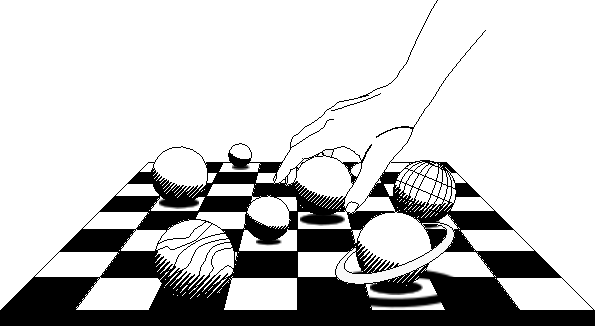
\includegraphics[width=0.8\textwidth]{frontispice-echiquier-celeste.pdf}

      %\vfill
      \vspace*{0.5cm}

      \begin{adjustwidth}{4.0cm}{4.0cm}
        \begin{center}
        \textsc{Dramatis personæ}
        \end{center}
        \footnotesize
   
        \setlength{\columnseprule}{0.5pt}
        \setlength{\CharWidth}{1.6cm}
        \begin{multicols}{2}
          %\raggedright
          \dodramperlist{}
        \end{multicols}

        \begin{center}
        La scène se déroule dans l’Arche envoyée il y a vingt-huit-milles ans depuis la Terre afin d’atteindre Proxima Centauri b.
        \end{center}
      \end{adjustwidth}

      %\vfill
      %\vspace*{1.5cm}

      \makeatletter
        \vspace{0cm}\large \@author

      \vspace{.5cm}\large \@date
      \makeatother


      \vspace*{2cm}
      \vfill
    \end{center}
    \restoregeometry
  \end{titlepage}


  \frontmatter


  \thispagestyle{empty}
  \pdfbookmark[0]{Page de garde}{garde}
  \null\vfill           % Pression du haut pour condenser les informations de crédit en bas de la page.

  \begin{center}
    {
    \Huge
     \MakeUppercase{
       Ascension d’\elena{} skylab}
       \vspace{0.5em}
       
       \MakeUppercase{{\em{}bâtard de l’Arche}
     }
     }
  \end{center}

  \vfill\null           % Pression du haut pour condenser les informations de crédit en bas de la page.
  \cleardoublepage
  
%  \ifodd\value{page}\thispagestyle{empty}\hbox{}\newpage\fi
  \thispagestyle{empty}
  \pdfbookmark[0]{Introduction}{dedicace}
  \null\vfill           % Pression du haut pour condenser les informations de crédit en bas de la page.
\addcredit{GFDL | \ccbysa{} | \ccby}{Käyttäjä:kompak}{https://commons.wikimedia.org/wiki/File:Pschent.svg}
  \begin{flushright}
    \begin{minipage}[t]{0.6\textwidth}%
%     \begin{center}
%       \phantom{\includegraphics[height=5.8em]{pegase.pdf}}
%     \end{center}

      %\lettrine{J}{e}
      \parshape=4
      0pt \textwidth
      0.1\textwidth 0.9\textwidth
      0.08\textwidth 0.92\textwidth
      0pt                \textwidth
      \noindent{}\raisebox{-\height+1.365cm}[0cm][0pt]{
        \hspace{-0.2cm}
\includegraphics[height=5.8em]{J-lettrine-pshent.pdf}%
      }%
      \hspace{-0.2cm}{\textsc{e}}
      me suis réveillé un matin avec le  souvenir d’un rêve étrange. C’était le songe d’une pièce qui s’ouvrait ainsi \enquote{Le Divin a donné à mon père un seul enfant. Le diable m’offrit alors en guise de cadeau de baptême.}, réplique prononcée par un personnage dont le nom me vint aux lèvres dès mon premier mouvement de paupière : \elena{}, \elena{} Skylab. Me revint aussitôt en mémoire la scène macabre du césar sur son lit qui, inconsolable, enlaçait le corps autant mutilé que sanguinolent d’une défunte femme.

      À cet instant, je ne savais ni qui était cet \elena{}, ni qui était le monarque, ni qui était la défunte, ni même où ils étaient.

      Je fis part de tout cela à un ami qui me fit remarquer \enquote{Tu as maintenant une pièce intéressante à écrire.}. Époussetant à peine les grains de sébum de ma caroncule, je lui répondis \enquote{Hélas.}.

%     \begin{center}
%       \includegraphics[height=5.8em]{pegase.pdf}
%     \end{center}
    \end{minipage}%
  \end{flushright}

  \vfill\null                % Espace vértical.

  \mainmatter
  % vim: syntax=tex
% aspell-ignore: trisuel, arca, jactata
%\addtocontents{toc}{\protect\enlargethispage{-40mm}}
\act

\scene

\StageDirII{\elena, \alexas}

\decors{La scène représente le module forestier de l’Arche qui reproduit une forêt de peupliers et de cyprès avec sur le lointain un gigantesque vitrail donnant sur l’espace.}
\StageDir{Sur ce vitrail qui est en fait un écran est projetée une vue en direct du foyer. On y perçoit de trois quart \elena{} de dos, si possible, dans un mouvement de traveling. Caméra à l’épaule tournant autour d’\elena{} jusqu’à révéler son visage pensif. \elena{} prend alors la direction de la scène où l’on le suit caméra à l’épaule, jusqu’à ce qu’il arrive côté jardin.}
\sceneinfo{Où \elena{} apprend à \alexas{} qu’il est né de façon naturelle.}

\begin{drama}
  \elenaspeaks Lorsque le Divin donna à mon père son premier enfant, le diable m’offrit alors en guise de cadeau de baptême. %\workingnote{S’adapter au fait que \roi a trois enfants au total, et reporter la correction dans le prologue.}

  \alexasspeaks Bonté du Ciel. Le Divin qui dans son infinie sagesse ne nous accable de déplaisirs sans les compenser par des réjouissances égales,  ne put affubler votre père d’un bâtard que pour le gratifier en retour par quelque motif d’égayement.

  \elenaspeaks Et pour cause, son déshonneur fut lavé à l’instant même où il se flétrit par ma venue au monde.

  \alexasspeaks Plait-il ?

  \elenaspeaks Madame ma mère est morte en couche.

  \alexasspeaks Qu’est-ce à dire que votre mère soit morte en couche ?

  \elenaspeaks Eh bien, je suis né de femme par voie pelvienne. 

  \alexasspeaks Messire \elena, vous badinez  ? %\workingnote{Explicationisme. La chose devrait être amenée plus finement qu’un cours magistral.}
                Depuis les vingt-huit-mille années que notre Arche a quitté la Vieille-Terre, nul humain ne put naitre en dehors des incubateurs, comme je vous l’ai enseigné. Protégée par d’épaisses cloisons en plomb que les premiers Voyageurs, nos ancêtres, ont embarqué, la méiose ne se déroule nulle part ailleurs sans que le rayonnement cosmique n’endommage le génome. Brillant prince, il ne sied pas aux esprits de votre rang de soutenir les inepties colportées par les agitateurs de la Cale. Ceux-là qui depuis le centre de l’Arche manigancent contre ceux que le destin a voulus puissants.


  \elenaspeaks Vous croyez cela ?


  \alexasspeaks Eh %\workingnote{Redite avec la précédente réplique d’\alexas. Les deux répliques gagneraient à être fusionnées en une seule.}
   bien, aucun homme de mémoire de Voyageur n’est né par voie pelvienne. S’il ne s’était trouvé les archives pour nous dire que les humains naissaient ainsi sur la Vieille-Terre, nous ne l’aurions probablement jamais su. Les quelques répugnants hardis qui s’y essayèrent n’obtinrent que d’odieux avortons dont les protéines sont tout juste bonnes à se verser dans le recycleur où se broient les chaires.

  Les personnes désireuses d’avoir un enfant selon leur génome s’adressent à l’incubateur qui en façonne un en couplant leurs gènes aux gènes compatibles. Votre père, pour vous avoir, a surement du mêlé ses gènes à des gènes d’une dame de la cour, et non à des gènes roturiers ce qui pourrait raisonnablement corroborer les informations qui vous parvinrent. Mais votre conception se sera déroulée dans l’incubateur, non à la manière des anciens humains.

  De grâce, ne soyez guère tenté par ces billevesées qui parcourent les allées et avenues de l’Arche. Assurément, ce n’est que la prudence de messire votre père qui a dû semer ces faussetés parmi les gens du commun afin de mieux entretenir la gueuserie où la nature nous commande de les maintenir.

  \elenaspeaks Grande est votre sapience, excellent \alexas{}, et vous n’usurpez point la réputation de docte parmi les doctes. Mais quoique modeste soit le peu de savoir que mon esprit faible ait pu emprunter au vôtre, je ne tarderai guère à rembourser ma dette didactique. Il se pourrait même que vous bénéficiiez d’intérêts.

  \alexasspeaks À n’en point douter. Je vous souhaite, pour vous et pour le bien de l’Arche, d’acquérir la sagesse, d’hériter celle de messire votre père. Mais prenez garde à ce que dans le chemin qui vous y mène, les embuches qui y sont semées \incise{et elles sont nombreuses} ne vous entrainent dans le bas-côté, celui pour lequel les gens du commun n’ont d’autre nom que celui de folie. 

  \elenaspeaks D’embuches, %\workingnote{Variante : \enquote{Plut au Ciel que les ennemis fassent pleuvoir davantage d’embuches devant moi, pourvue que le gouffre qui me sépare de la gloire en devienne comblé.}.}
  je suis heureux qu’il y en ait de multiples, car %le trône sur lequel je m’établirais ne sera point battit d’un autre matériau.
  il me faudra bien de ce matériau pour bâtir le trône sur lequel je m’établirais.
  %Compte à vous qui tirez votre science de la haute académie, vous n’aurez pas attendu longtemps avant de recevoir le premier acquittement du fort brillant enseignement que vous me prodiguâtes.
%  Plut au Ciel que les énemis fassent plevoir les embuches devant moi, car le gouffre qui me sépare de la gloire devient chemin lorsque les embuches viennent le combler. Et s’il devait me paraitre encore trop éscarpé, c’est que j’aurais failli à me faire assez d’énemis.

  \alexasspeaks Il est bon que vous me fassiez les confidences d’aussi hardies ambitions afin que je vous exhorte aussitôt à les réprimer. Votre bâtardise, quoique d’escient récent, vous prive du trône; et messire votre père a tranché en faveur de Son Altesse votre sœur. Les arrêtés de Sa Majesté ne se discutent que dans les entrailles du recycleur.

  \elenaspeaks Pour l’avoir de ma main actionné, je vous dispenserais de cette mise en garde.

  \alexasspeaks C’est pourquoi mon sermon n’est point assorti de remontrances. Au contraire, je vous incite à exulter.
  Car c’est avec joie que vous embrasserez la carrière militaire dont Sa Majesté vous veut gratifier. Et c’est en général d’armée que vous servirez votre souveraine, Madame votre sœur.

  \elenaspeaks Gloire à la princesse héritière.

  \alexasspeaks Gloire à elle.

\end{drama}

\scene

\StageDirII{\elena, \alexas, \general{}}

\sceneinfo{Où \general{} s’avère avoir connaissance de la bâtardise d’\elena{}.}

\begin{drama}
  \generalspeaks D’ordinaire, je récompense mes lieutenants lorsqu’ils se font pareilles messes basses et honnis les ennemis qui s’y adonnent. De quel camp êtes-vous ? 

  \alexasspeaks De celui du roi, assurément.

  \generalspeaks Ce sont là de sages paroles qui honorent ton intellect.

  \elenaspeaks \general, notre ami, quel plaisir exquis de te savoir des nôtres. Et la jouissance s’en accroit à mesure que la crainte inspirée par ton nom aux ennemis est grande.

  \generalspeaks Ah, plût au Ciel que de pareilles opinions puisse se hisser du fis au père et, dans cette ascenssion, faire fi du plafond de la batardise.

  \alexasspeaks Comment donc \general ? Se pourrait-il que dans ce que me rapporta messire \elena il y ait du vrai ? Et que dès lors vous eûtes été mis dans la confidence ? 

  \generalspeaks
  Il l’a bien fallu, tant la honte que sa venue au monde inspira à son géniteur ne put se suffire des pages arrachées à vos grimoires pour se draper. Songez que ces mêmes pages-là qui servirent à l’emmailloter faillirent être son linceul.\label{sec:metaphore-papier-linceul}
  Et quelqu’honorabilité eut-il pu acquérir au travers de l’éducation studieuse et raffinée de votre plume, cette dernière n’aura pas été aussi aiguisée que mon glaive lorsqu’il s’est agi de couper les oreilles qui ouïrent l’inaudible secret, autant que les langues qui risquèrent de le divulguer.

  \alexasspeaks À pareil compte, j’eus voulu être tenu à l’écart de pareille connaissance. N’en ai-je pas acquis de bien suffisantes pour risquer de perdre et ma langue et mes oreilles ?

  \generalspeaks Notre souverain a jugé du contraire. Désireux de faire monter sa fille sur le trône, il a estimé que le dos d’un bâtard reconnu par tous comme bâtard était un marchepied à la mesure de sa gloire. À la fois prompt à affermir la souveraineté de sa fille, et suffisamment humiliant à son fils pour qu’il ne puisse prétendre au trône.

  \elenaspeaks Tant de clémence est digne d’un souverain éclairé.

  \alexasspeaks En somme, il lui enlève l’honneur et lui laisse la vie. Et il faudrait alors que la cour et le peuple sachent la chose. De telle sorte que, délégitimé du trône, notre souverain consente à le laisser en vie.

  \generalspeaks Notre souverain le veut. Mais encore, il ne voudrait pas que la chose s’ébruite trop vite, ni trop certainement. Il faudrait que se murmure la nouvelle de son illégitimité, qu’elle soit divulguée au peuple avec si peu de conviction que certains y croient, d’autres s’en méfient, mais que la plupart hésitent. Qu’elle paraisse comme une vilaine rumeur qui se murmure davantage qu’elle ne se clame.

  \alexasspeaks Ainsi,  sera-t-il suffisamment compromis pour le trône, mais encore suffisamment aimé pour être de l’état-major. Il y’a grande rigeure à faire tenir pareil équilibre.

  \generalspeaks \alexas, sage d’entre tous, votre sagacité fera toujours merveille. Et le roi, vous le démontrez à l’instant, ne s’est pas trompé en  vous désignant pour instiguer la chose en funambule émérite du royaume.

  \alexasspeaks Pour servir notre roi et épargner mon disciple, je dévierai les planètes de leurs orbites.

  \StageDir{\alexas regarde vers son terminal brachial.}

  \alexasspeaks Permettez messires ? Je viens de recevoir une épitre du cabinet royal exigeant que  j’en prenne connaissance dans des conditions de confidentialité.

  \generalspeaks Mais faites donc.
\end{drama}

\scene

\StageDirII{\elena, \general}

\sceneinfo{Où \elena{} promet à \general{} qu’il convaincra le roi d’en faire le chef des armées.}

\begin{drama}
  \generalspeaks \elena, mon doux ami, que ne me suis-je ébaudi de vous entendre tantôt vanter mes talents militaires.

  \elenaspeaks Qu’est-il besoin de vanter lorsque les cliquetis de vos armes en action qui s’oient encore dans l’armée et dans le peuple plaident bien assez votre cause ?

%  \generalspeaks Il  ne le feront assez que lorsque notre souverain, votre père, en sera autant convaincu que vous.
  \generalspeaks Ils  ne le plaideront assez que lorsqu’arrivés aux oreilles de notre souverain, votre père, ils l’auront convaincu tout autant que vous l’êtes.

  \elenaspeaks Cela viendra. S’il ne fait pas de doute à mes yeux que votre place à la tête des armées est dans l’intérêt l’Arche entière, croyez que mon père n’aura pas sitôt fait d’être acquis à mon opinion.

  \generalspeaks Comment donc ? N’est-ce pas de lui que vous la tenez ?


%  \elenaspeaks Il n’en est pas encore convaincu. Mais je m’emploie à l’en convaincre.
  \elenaspeaks Cette opinion n’est pas encore tout à fait sienne. Mais je m’emploie à la lui faire acquérir.

  \generalspeaks 
  Ah, la sinistre existence. J’eus l’audace de croire que de pareilles idées n’étaient vôtres que parce que vous les héritiez de votre père.

  Mais si donc ce n’est pas le sang qui transmit d’aussi louables pensées du père au fils, ne se pourrait-il que la salive les élevât du fils au père ?

  \elenaspeaks Cela se peut.

  \generalspeaks Cela se doit. Je ne le convainquis de dévoiler votre adultérine conception, préservant ainsi votre vie, que pour qu’en échange vous le persuadiez de me nommer à la tête des armées. Et je ne trouve pas votre part du marché si onéreuse au prix que j’obtins pour vous.

  \elenaspeaks
  Il est plus aisé de convaincre un père d’épargner la vie d’une progéniture, même malaimée, que de l’inciter à évincer son enfant préféré. Plus encore si l’éviction se fait au profit d’un étranger avec qui il n’a point en partage le sang.

  Néanmoins, je tiendrais ma part du marché. Je suis un homme d’honneur.

  \generalspeaks Il serait souhaitable que celui qui ne fit point preuve d’honneur dans la naissance en fasse dans son existence.

\end{drama}

\scene

\StageDirII{\elena, \general, \alexas}

\sceneinfo{Où \elena{} donne quelques conseils à \general{} pour convaincre le roi.}

\begin{drama}
  \alexasspeaks Le roi nous voudra voir dans la salle du trône.

  \elenaspeaks À la bonne heure. J’expliquais justement à notre hôte que je tâcherais de convaincre notre souverain de le mettre à la tête des armées, mais que cela serait difficile.

  \alexasspeaks Le roi, excellent \general, en outre des incitations de monseigneur \elena{}, sera confronté au parti de la reine qui plaidera en faveur de sa fille.

  \elenaspeaks Voilà pourquoi il vous faudra faire étalage de compétences qu’il sera prompt à brandir à ses contradicteurs en guise d’argument.

  \generalspeaks Et si, convaincu de la faiblesse de la princesse, il ne vienne à nommer son autre fils légitime à la tête des armées ? Après tout, en tant que fils de la reine, le parti de cette dernière le soutiendra tout autant que la princesse.

  \elenaspeaks Encore faudra-t-il réussir à le tirer de l’amoncèlement de putains sous lequel il est constamment enseveli.
  Il en commande régulièrement à l’incubateur qui lui en fournit des exemplaires au génome tout juste stable pour vingt-cinq
 %\workingnote{Si l’on opte pour les nombres hexadécimaux, il faudra se demander s’ils sont à généraliser partout.}
  ans d’existence, avant que leurs protéines ne soient de nouveau versées au recycleur. Mais il en use tant qu’après deux ans seulement, elles ont l’air d’être en fin de vie.

  \StageDir{Rires.}

  \generalspeaks \direct{Vers \elena} Compte à vous, il est évident que vous feriez de l’ombre à Son Altesse votre sœur. Raison suffisante qui vous écarte de l’état-major.

  \elenaspeaks Rien n’est plus vrai. Votre seule rivale est la princesse \princesse. Auprès de notre souverain, montrez-vous au fait des positions de l’ennemi, des hypothèses de la stratégie qu’il mettra en œuvre. Et notamment, insistez sur la nécessité d’engager davantage d’ingénieurs à la cyberguerre. Ce point précis lui tient à cœur. 

  Dites-lui de doubler les effectifs et il vous reprochera de ne pas vouloir les tripler. Ma sœur à l’humeur sanguine ne croit qu’en l’artillerie et l’assassinat. Lorsque devant la cour elle sous-estimera hautement l’importance de la cyberguerre, vous vous distinguerez. Et ceux qui vous auront jusqu’alors été hostiles n’auront plus la verve de soutenir d’autres que vous.

  \intrat{\page}

  \pagespeaks \direct{S’adressant à \general} Seigneur, votre chapelier est prêt.

  \generalspeaks Avant de ne devoir vous laisser messire \elena{} pour m’adonner aux joies sartoriales, oserais-je abuser de votre amabilité en vous demandant quelle couleur pourrait seoir à la coiffe que je commande, celle que je porterais au retour de la victoire ?

  \elenaspeaks La lazulite, couleur rare, couleur de la victoire, ne saurait que trop affermir votre gloire. Oserais-je suggérer l’adjonction d’un uræus sur le front en guise de protection contre vos ennemis ? Quoique je vous recommande toutefois de prendre garde à votre chapelier, l’on dit les gens de cette profession fous.

  \generalspeaks   Si la folie eut été contagieuse, je craindrai davantage pour eux  qu’ils ne la contractassent de moi ! Car je me soumets si aisément aux sirènes des fripes et parures qui m’appellent que l’on ne pourrait me suspecter d’être mieux douté de raison qu’eux. Que voulez-vous ? J’ai toujours cédé à l’appel de la frivolité. Après tout, Arès dont je suis disciple, n’est-il pas amant d’Aphrodite la bien parée ?

%  \generalspeaks Ah, messire \elena{}, comment tant de raffinement peu côtoyer dans un même esprit autant de génie politique ? Mais avant de n’y répondre, messire \elena{} tachez de tenir vos engagements.
%  Compte à moi, je me soumets aisément aux sirènes des fripes et parures qui m’appellent. Que voulez-vous ? J’ai toujours cédé à l’appel de la frivolité. Après tout, Arès dont je suis disciple, n’est-il pas amant d’Aphrodite la bien parée ?

  %\elenaspeaks Ne soyez point modeste. Vous êtes un esthète avisé, voilà tout. Mais prenez toutefois garde à votre chapelier, l’on dit les gens de cette profession fous.
  \exit{\general}

\end{drama}

\scene

\StageDirII{\elena, \alexas}

\sceneinfo{Où \alexas{} confirme à \elena{} que l’expérience de fécondation est réussie.}

\begin{drama}
  \alexasspeaks \direct{Complétant la précédente réplique de \general}Amants d’une liaison adultérine.

  \elenaspeaks Pour laquelle l’habileté d’un Héphaïstos industrieux ne tardera pas à forger de sinistres desseins.

               À cette fin, \alexas, t’es-tu bien assuré de la chose dont nous nous entretînmes ?
  
  \alexasspeaks Oui Sire, \catin{} porte bien en son ventre l’enfant. La méiose s’est déroulée avec le succès que nous escomptions et son génome est stable.

  \elenaspeaks Puisse cet enfant vivre longtemps, devenir fécond et prolifique.

  \alexasspeaks
  \begin{minipage}[t]{\linewidth}
    Que ces dires soient reportés aux annales,\\
    En hiéroglyphes et en ossécaille.
  \end{minipage}
\end{drama}

\scene


\StageDirII{\reine, \princesse}

\decors{Dans un boudoir richement paré avec de larges ajours donnant sur l’espace.}

\sceneinfo{Où \reine{} exhorte \princesse{} à réclamer le commandement de l’armée.}

\begin{drama}
  \reinespeaks \princesse, ma fille. Vous êtes appelée à siéger sur le trône du \campprincipal{}. Or, votre bâtard de frère fait preuve de tant de largesses auprès du peuple que sa renommée risque de vous faire de l’ombre. Il vous faut gagner en autorité par des succès militaires.

  \princessespeaks Je n’ai jamais désiré, mère, autre chose que me soit confié un bataillon en compagnie duquel je me lancerais d’entre les artères de l’Arche pour infliger à l’ennemi des pertes qui lui feront craindre jusqu’à mon nom. Je voudrais que lorsqu’ils élèvent leurs enfants, ils m’utilisent comme figure d’épouvante ; ils leurs diraient que \princesse{}  l’ogresse viendrait se nourrir de leurs protéines s’ils ne sont pas obéissants. Que dans tout le \campprincipal{}, les seuls à appréhender avec crainte les batailles que je mène soient les employés du recycleur auxquels je donnerais tant de labeur par la profusion de chair ennemie qu’il leur faudra traiter.

  \reinespeaks Ah, que l’oreille d’une mère est délicieusement chatouillée à de pareils dires !

  \princessespeaks Mais en dépit de ma détermination, n’avions-nous pas meilleur compte d’envoyer \elena{} au broyeur plutôt que de se soucier de la faveur qu’il a au sein du peuple ?

  \reinespeaks Votre père en a décidé autrement malgré les nombreuses diatribes que j’ai prononcé à son endroit, et les non moins nombreuses compagnes de dénigrement que mes agents ont menées contre lui.

  \princessespeaks Mon père est un faible et nous devrions passer outre sa décision.

  \reinespeaks Réprimez vos propos, ma fille. La loi de l’Arche que nous avons reçu dès le Jactum est au-dessus de nous tous et consacre la primauté aux décisions de votre père. Et n’oubliez pas que c’est par sa décision que vous êtes héritière présomptive, car j’ai manigancé afin que vous soyez sa fille préférée. Et c’est aussi par sa décision que vous pourrez être déchue.

  \princessespeaks Qu’importe, je m’accommoderais bien de succès militaires pour assoir mon autorité et tolèrerais \elena{} comme ministre sous mon père.

  \reinespeaks Lorsque votre père ne sera plus des nôtres, il vous sera loisible de prononcer sa disgrâce.

  \princessespeaks Je %\workingnote{Variante avec violence sexuelle incestueuse : \enquote{Pourquoi donc quand je pourrais l’appeler tous les jours à s’agenouiller devant mon trône où il léchera la vulve de sa reine ? Ainsi tout le monde reconnaitra ma souveraineté.}.}
  l’enverrais alors au recycleur qui récupèrera ses protéines. Oh, mère, je me vois déjà récupérer ses restes du recycleur pour en faire le terreau des bégonias que je ferais pousser dans un pot en forme de barque solaire à la salle du trône. Sans mentir, je vois là une enivrante perspective.

  \reinespeaks Ne vous ai-je pas appris, ma fille, à ne jamais faire preuve de cruauté inutile ? En gravissant les marches vers le trône, l’on doit se délester de ces basses aspirations tout juste bonnes aux gens du commun.

  Vous tiendrez ces passions pour des liens qui nous retiennent de gravir les marches du trône.%
  Vous intronisée, plus que jamais vous le souhaiterez vivant, afin qu’en captif de votre cour l’humiliation qu’il vivra chaque jour soit un enseignement aux hardis qui voudraient attenter à votre pouvoir. Compte aux bégonias, s’ils vous plaisent tant, à quoi bon attendre le trépas de votre frère ? Je vous en ferais ramener dès aujourd’hui. Que vous importe le terreau qui les aura nourrit.

  \suivanteprincessespeaks Madame, messire votre père vous fait appeler à la salle du trône.
%
%  \princessespeaks Pourquoi donc quand je pourrais l’appeller tous les jours à s’agenouiller devant mon trône où il léchera la vulve de sa reine ? Ainsi tout le monde reconaitra qui est souverain.
%
%  \reinespeaks Faites cela et c’est moi qui lui maintiendrais la tête.
%
\end{drama}

\scene

\StageDirII{\roi, \reine, \princesse, \elena, \alexas, \general}

\decors{Dans la salle du trône.}

\sceneinfo{Où le roi attribue le commandement de l’armée à \princesse.}
\begin{drama}
  \roispeaks Ah ma fille adorée. Tenant d’une main la lance, de l’autre le bouclier, je voudrais que comme les déesses de la Vieille-Terre te pousse un troisième bras dont je te ferais saisir le gouvernail de l’arche toute entière. Et que le \campoppose{}, tremblant à la seule évocation de ton nom, ne te désigne que par périphrase.

  Te voici maintenant dame, et je voudrais te confier la bataille où tu accomplira tes premiers faits d’armes.


  \princessespeaks Oui père. Et à défaut de troisième bras, c’est la tête casquée que je me présente à vous. Vous soustrayant bien respectueusement à vous le regard noir que pour mieux le réserver au \campoppose{}.

  \roispeaks Ah viens vers moi que je t’embrasse, ma fille. Si la certitude de votre supériorité au commandement m’est acquise, il me faut être un roi impartial. Voilà devant toi \elena{}, ton frère dont le peuple veut faire son vengeur, et \general{} dont les hauts faits ne sont plus à narrer.

  \reinespeaks Mon roi et époux. N’y voyez que mon souci de l’intérêt supérieur du royaume, si ma maladresse me laisse paraitre offensante. Mais il se murmure des choses au sujet de Sire \elena{} que je tiens en plus haute estime que mes propres enfants.

  \roispeaks Que se murmure-t-il ?  Ce qui intéresse les affaires de l’État se doit d’être dit hautement.

  \reinespeaks Il se dit qu’il a des qualités qui ne s’accommodent guère de l’office auquel vous le voulez dévolu.

  \roispeaks Mon épouse, il n’appartient pas à la dame du plus haut rang de verser dans le complotisme auquel s’adonne la lie de l’humanité qui pue la suie et la sueur dans la Cale.
  En tout état, la vertu cardinale qui incombe au stratège est la stratégie,  et c’est pourquoi je veux d’abord vous interroger \general{} sur la chose à faire.

  \generalspeaks Sire, l’on ne peut mieux s’exprimer que vous. Mes faits d’armes plaident pour l’habileté que j’ai à vous servir comme vous le dites. L’armée est familière de mes mœurs millitaires et sait agir sous mon commandement avec la promptitude qui fit ses succès et votre gloire. La stratégie que je propose est celle qui fera notre victoire comme elle le fit naguère : la surprise. Ayant l’habitude de mener nos attaques par les voies et artères internes, je préconise cette fois-ci d’emprunter la voix de l’espace extérieur. Les ennemis qui auront massifié leurs troupes devant les voies intérieures se retrouveront désemparés lorsque leurs modules civils se retrouveront exposés à notre artillerie. Ainsi votre victoire sera faite et je gage que dans deux ou trois batailles, vous n’aurez pas assez d’un seul séant pour vous établir sur les deux trônes du \campprincipal{} et du \campoppose{}.

  \roispeaks Cela est bon, et ma fille a élaboré un pareil stratagème, à quelques variantes près. Mais encore, tout aussi surprenant fut-il, votre précédent stratagème a pourtant engendré nombre de pertes parmi nos soldats. Vos plans prévoient-ils quelque chose pour soulager la production de soldats dans l’incubateur ?

  \generalspeaks Mon roi, votre général ne saurait que trop anticiper vos questions afin d’y pourvoir avant qu’elles ne soient posées. Aussi pensé-je qu’il faudrait tripler le nombre de nos cyber-ingénieurs afin de mieux connaitre les communications de l’ennemi. Il est important que notre présence sur le cyber-espace soutienne l’action de notre artillerie.

  \roispeaks Hmm. Tripler est bon. Je vous aurais cru prompt à quadrupler.

  \princessespeaks Père, mes plans comme vous le savez sans doute, prévoient de décupler nos cyber-agents. Ils seront répartis comme suis : un tiers sera dévolu au sabotage des engins de l’ennemi, un tiers sera chargé du décryptage, et un tiers veillera à la robustesse de nos chiffrements cryptographiques.

  \StageDir{\general{} se retourne étonné.}

  \roispeaks Voilà qui est encore meilleur. Compte à vous mon fils, vous n’avez pas dis un mot depuis tout à l’heure. Attitude au demeurant sage et louable qui maintient l’ennemi sous le voile de guerre, mais qui devant vos supérieurs doit faire place à la volubilité. Dites-moi, que pensez-vous de nos cyber-défenses ?

  \elenaspeaks Ma foi, père, je ne saurais trop quoi dire. Dans mes classes, l’on m’apprit trois choses : l’artillerie, encore l’artillerie, toujours l’artillerie. Et c’est histoire de cyber-défense, de cyber-attaque, me donnent un cyber-tourni. Je préconise comme tout le monde d’attaquer depuis l’extérieur pour faire la surprise. Cela est évident, mais je doute que dépenser de l’argent dans des bigleux qui pianotent sur leur clavier fasse avancer notre cause. D’autant que cet argent serait mieux employé à venir en aide aux plus nécessiteux.

  \roispeaks La chose est entendue. Ce sera ma fille, la princesse \princesse{} qui mènera nos forces, avec l’aide de la Profondeur du Cosmos.

  \speaker{Tous sauf le roi}
  \begin{minipage}[t]{\linewidth}
    Que ces dires soient reportés aux annales,\\
    En hiéroglyphes et en ossécaille.
  \end{minipage}


  \exeunt{\reine{} ainsi que \princesse{} d’un côté et \elena{} ainsi qu’\alexas{} de l’autre}
\end{drama}

\scene

\StageDirII{\reine, \princesse}

\decors{Dans l’arrière-chambre du trône.}
\sceneinfo{Où \reine{} donne un dernier conseil à  \princesse.}
\begin{drama}
  \reinespeaks Ah ma fille, si je n’avais soudoyé ce lieutenant de \general{} nous aurions eu probablement plus de mal à l’évincer. C’est une leçon pour l’avenir, 
  tes espions n’auront les lèvres déliées qu’autant que ta bourse le sera à leur endroit.

  \princessespeaks S’il n’était pas mal avisé de laisser des traces écrites, je tiendrais un mémoire de vos leçons. Encore heureux que vous agîtes de la sorte. Car ces histoires de cyber-choses sont tout juste bonnes pour la vieille génération. J’eus même de l’admiration pour  \elena{} dans la salle du trône, et je l’aurais bien soutenu s’il n’en alla de mon intérêt de me retenir. Il fallait bien un sénile comme \general{} pour en avoir l’idée.

  \reinespeaks Pour le reste, tenez tout de même compte de son plan. Prenez-le en entier et faites-le votre. Ne négligez rien de votre cyber-attaque ni de votre cyber-défense.

  \princessespeaks Veuillez, mère, appliquer la ruse de Loki dans la cour, et me laisser frapper de la force de Thor sur le champ de bataille. Vous connaissez votre art et moi le mien.
\end{drama}

\scene

\StageDirII{\elena, \alexas}


\decors{Dans le couloir au sortir de la salle du trône.}
\sceneinfo{Où \elena{} révèle que \general{} n’aura pas le commandement de l’armée.}
\begin{drama}
  \alexasspeaks Sire, Sire, venez plus près de crainte que l’on nous entende.

  \elenaspeaks Qu’as-tu à me dire, précepteur ?

  \alexasspeaks Le roi n’a pas nommé \general à la tête de ses armées.

  \elenaspeaks Non, il ne l’a pas fait.

  \alexasspeaks Or vous avez promis au général qu’il sera désigné.

  \elenaspeaks Je lui ai promis de convaincre mon père de le nommer à la tête des armées. Ne l’ai-je pas fais ?

  \alexasspeaks Si, vous le fîtes.

  \elenaspeaks L’intéressé n’était-il pas présent lui-même pour s’en rendre compte ?

  \alexasspeaks Il l’était.

  \elenaspeaks Qu’a-t-il à me reprocher maintenant que ma part du marché est remplie ?

  \alexasspeaks Il risque d’être fort mécontent.

  \elenaspeaks La belle affaire. Nous avons tous de nombreuses raisons de l’être constamment. Et les ouvriers et les gens de la Cale en ont davantage que nous.

  Va maintenant, \alexas, va en mon nom ordonner moult virements monétaires aux nécessiteux au sein du peuple.

  \alexasspeaks Vos finances, Sire, sont en déséquilibre. Et le peuple, déjà reconnaissant des largesses que vous lui fîtes vous soutient déjà. Avec quels fonds comptez-vous encore distribuer l’aumône ?

  \elenaspeaks Ne te soucie guère de cela, j’en fais mon affaire. Réunis l’ensemble de mes capitaux dispersés sous les différents prête-noms et distribue-les immodérément. 
  Donnes-en à ceux dont les organes sont en fin de service. Ceux dont les télomères de leurs chromosomes s’effilochent. Mais surtout veille à ce que le peuple sache que je suis son bienfaiteur.

  \alexasspeaks Voudriez-vous regagner en popularité afin que le roi vous nomme à la tête des armées et prendre ainsi la place de \general ?

  \elenaspeaks Dieu du cosmos, non ! Plus je m’attirerais les grâces et la bienveillance de la populace, plus la reine décuplera d’efforts auprès du roi pour le convaincre de maintenir sa fille à la tête des armées. Je me prémunis du cas où  l’idée saugrenue de changer d’avis lui prendrait. Ainsi, ce sera bien ma sœur et nulle autre personne qui ira au combat.

  \alexasspeaks Mais donc, vous n’avez rien prévu pour que \general{} dirige nos armées ?

  \elenaspeaks Non, je n’ai rien prévu pour cela.
               J’ai même prévu l’inverse.

  \alexasspeaks Sire, tout disciple que vous êtes, j’avoue percevoir moins clair dans vos desseins que dans la profondeur de l’espace.

  \elenaspeaks Vous qui juchés haut sur la vigie avez la connaissance de l’avenir et du lointain, ne pouvez percevoir ce qui se trame sous vos pieds dans la Cale.
\end{drama}


%\Scene{--- Épître d’\elena{} à l’état-major de \campoppose{}}

\scene

%\StageDirII{Épître d’\elena à l’état-major de \campoppose{}y}
\StageDirII{Première épître d’\elena à l’état-major de \campoppose{}}


\decors{\elena{} envoie à l’armée tribordienne les informations sur le plan d’attaque de \princesse{}, sous l’identité secrète d’un traitre.}

\sceneinfo{Où \elena{} trahit son camp en révélant à l’ennemi les positions de l’armée.}\nopagebreak

\begin{quotation}
  \ttfamily\RaggedRight
  \noindent{}Date : 8 trisuel 2871 \emph{ab Arca jactata}%\footnote{Correspondant au huitième jour, du troisième mois, de l’année 28871 après le lancement de l’Arche.}
  \\
  De : L’Informateur\\
  À : État-major du royaume de \campoppose{}\\
  Objet : Plan d’attaque du \campprincipal{}\\
  Condensat : 6b09816e4b37dc954d0023d020216c13\\
  Authenticité : Signature cryptographique vérifiée\\
  Pièce jointe : plan-dattaque-de-\campoppose{}.papyrus
  \nopagebreak\vspace{1em}

  De l’Informateur à l’état-major de \campoppose{}, salut.
  \nopagebreak\vspace{1em}

  Excellences, les informations dont je dispose font état de la massification des troupes du \campprincipal{} près des bouches de sorties extravéhiculaires augurant d’une attaque par le dehors. Mes investigations permirent de mettre la main sur le plan complet de la bataille qui sera menée par la princesse héritière présomptive du trône de \campprincipal{} dont vous trouverez copie en attachement à cette épître.

  Le subterfuge prévoit qu’elle ne sera pas physiquement présente dans le vaisseau de guerre amiral mais sur l’une des vedettes de l’aile gauche de l’armada. En outre, le tiers de la flotte demeurera stationné à l’intérieur du module forestier. Or cela est un affront aux traités de guère stipulant que les modules écologiques ne devraient jamais endosser de fonction militaire. Aussi me suis-je laissé dire que pareille infraction au droit militaire vous octroyait le droit d’attaquer les premiers, ce qui affaiblirait le moral de vos ennemis.

  Eu égard à la justesse de mes précédents rapports et à l’intérêt stratégique exceptionnel que contient le présent rapport, je vous demande une rétribution s’élevant à trente-mille cosmis.

  \nopagebreak\vspace{1em}
  Vie, prospérité, santé.

  \nopagebreak\vspace{1em}
  \hfill Votre dévoué informateur.
\end{quotation}


% \newgeometry{left=0mm,right=0mm,top=0cm,bottom=0cm}
%   \addcredit{\ccbysa}{Fenn-O-maniC}{https://commons.wikimedia.org/wiki/File:Arms_of_Oxfordshire_County_Council.svg}%
%   \addcredit{\ccbysa}{Trondivers}{https://commons.wikimedia.org/wiki/File:T08_Grossherzog.svg}%
%   \begin{figure}[p]% will be the left-side figure
%       \adjincludegraphics[width=\textwidth,trim={0 0 {.5\width} 0},clip]{courone-ensanglantée.pdf}
%   \end{figure}
%   \begin{figure}[p]% will be the right-side figure
%       \adjincludegraphics[width=\textwidth,trim={{.5\width} 0 0  0},clip]{courone-ensanglantée.pdf}
%   \end{figure}
% \restoregeometry

%\addtocontents{toc}{\protect\newpage}
%\addtocontents{toc}{\protect\enlargethispage{\baselineskip}}
\addtocontents{toc}{\protect\pagebreak} % ATTENTION ajustement conjoncturel
\act
%\chapterinfo{TEST}

\scene

\StageDirII{\elena, \alexas}

\sceneinfo{Où \elena{} et \alexas{} conjecturent de la réaction de \general{}.}

\begin{drama}
  \choirspeaks
  \begin{minipage}[t]{\linewidth}
      Les fleures du mal éploient leurs pétales\\
      Sous les hospices fatales\\
      Qui noircissent le ciel d’une nuée\\
      D’espérance dénuée.\vspace{1em}

      Dressant leurs épines vers le ciel\\
      Comme autant d’épées triomphantes\\
      Qui mènent la captive infante\\
      Vers la table sacrificielle\vspace{1em}

      Là où ayant humé\\
      Autant les flammes infernales\\
      Que le vent hiénal,\\
      Elle se verra inhumée.\\
  \end{minipage}

  \alexasspeaks Sire, excusez la hardiesse de votre serviteur, mais je crains que \general{} ne vous tienne tout de même rigueur.

  \elenaspeaks \direct{Éxaminant entre ces doigts la dame des figurines de Lewis} Et moi, je gage, précepteur, qu’il viendra tout au contraire me présenter une vive reconnaissance.

  \alexasspeaks Pour l’avoir exclu du commandement ?

  \elenaspeaks Pour lui avoir épargné la mort.


  \intrat{\disciple{} en catastrophe}

  \disciplespeaks \direct{En catastrophe} Sire, Sire, des choses graves se déroulent. Vous devriez vite vous rendre à la salle du trône en compagnie de maitre \alexas.
\end{drama}

\scene


\StageDirII{\elena, \alexas, \general}

\sceneinfo{Où \elena{} et \alexas{} rencontrent \general{} dans un couloir.}
\decors{Marchant dans un couloir de l’Arche.}\nopagebreak[4]
\begin{drama}\nopagebreak[4]
  \nopagebreak[4]\generalspeaks \nopagebreak[4]\direct{Allant à la rencontre d’\elena} Messire, oh messire, que la grâce du cosmos tout entier soit avec vous en ces temps troubles.

  \elenaspeaks L’on nous attend à la salle du trône, nous devons nous y presser.

  \generalspeaks L’on m’y attends moi aussi. Je vous suis, doux beau Sire.

  \alexasspeaks L’on m’annonce de funestes nouvelles. Certains de nos modules subirent de lourdes destructions. En savez-vous plus général ?

  \generalspeaks L’on m’apprit que le roi est dans de profonds abattements et mes fidèles lieutenants me pressèrent de me rendre auprès de lui.

  \alexasspeaks \direct{Bas à \elena} Auriez-vous, Sire, des informations que je méconnaitrais ?

  \elenaspeaks Qu’importe que je les ai, précepteur, lorsque vous les découvrirez dans l’heure. Songez plutôt au vizirat qui sera bientôt le vôtre.
\end{drama}


\scene


\StageDirII{\roi, \reine, \elena, \alexas, \general, \suivantes, \kingsgards}


\decors{Dans la sale du trône, où le trône s’est escamoté sous la forme d’un lit en marbre disproportionné sur lequel \roi{} est allongé enlaçant dans une vision d’horreur le corps inanimé et sanguinolent de \princesse. Sur un côté, se trouve un groupe formé des suivantes de la princesse en habits sacrificiels.}

\sceneinfo{Où \roi{} se lamente de la mort de sa fille.}

\begin{drama}
  %\StageDir{La scène s’ouvre sur les pleures et lamentations des suivantes de la princesse}

  \elenaspeaks \direct{S’approchant vers le lit du roi} Qu’est-il…

  \kingsgardsspeaks \direct{En croisant les hallebardes} Halte !

  \roispeaks \direct{Enlaçant dans d’inextinguibles larmes le corps inanimé de \princesse{} morte qui le tache de sang et tache le lit.}  Ah ma fille, mon seul enfant, où es-tu partie ? Et pourquoi ne daignes-tu plus bouger, ne plus m’adresser une seule parole, un seul sourire ? Rah, peste soit du \campoppose{}. Maudits soient-ils, qu’ils soient jettes vifs, avec le souffle à la bouche dans la vacuité sidérale. Je voudrais que vos chairs ne soient jamais recyclées et ne renaquissent  pas en plantes. Mais toi ma fille, ma puissante fille, se pourrait-il que je doive te léguer au recycleur ? Je composterais ton corps dans le plus fleuri des vergers qui donnera des fleures dont on assaisonnera nos royaux plats et les festins donnés à la noblesse. 
  Comment me résignerais-je à cette idée quand avant hier encore, parée d’électrum et de lazulite tu batifolais avec les lionceaux du zoo qui te mordillaient les mèches de cheveux noirs ? Quand hier encore adolescente, l’on voyait les têtes  de tes amants rouler à terre à peine après que tu ne t’en aies été repue et qu’avec tes rires inextinguibles se joignaient les nôtres ?

  Avant que ces souvenirs aillent au recycleur, il faudra attendre longtemps. Or tu es puissante, n’est-ce pas ma fille ? Tu terrasseras encore maints ennemis avant que ton souffle cesse. Ma fille, mon seul enfant, chair de ma chair, un avenir brillant t’attend. Et à ton commandement, tu n’auras pas seulement le royaume de \campprincipal{} mais l’Arche entière que tu guideras jusqu’à Sion.

  Ah, vile existence, maudite existence. Pourquoi, par tes décrets capricieux, nous fais-tu jouir du pouvoir, du bonheur, d’une progéniture aimée, si ce n’est pour mieux nous accabler lorsque tu nous les retire ? Amour qui ne vaut qu’au jour où il nous est dérobé. Ah, que le sceptre démange la main droite qui le tient lorsque la gauche ne peut balancer le berceau. Ô vie, ou donne-moi tout, ou prive-moi de tout. Mais ne me nargue pas  avec la vaine consolation du pouvoir lorsque plus rien ne vaut d’être gouverné. Ô détestable vie.

  \reinespeaks \direct{S’approchant du lit royal} Mon roi et époux, dans l’incommensurable deuil qui nous touche tous les deux, père et mère, il nous faut songer à livrer la dépouille de notre défunte fille au recycleur et donner au royaume un héritier. Vous avez encore un fils…

  \roispeaks Comment ? Voudriez-vous que l’on usurpe le trône de ma fille ? Arrière infâme.

  \kingsgardsspeaks \direct{En croisant les hallebardes qui entravent la reine} Halte !

  \reinespeaks Mon roi, je suis aussi éplorée que vous. Mais songez à l’État. Le peuple de la Cale au sein duquel gronde la révolte, la noblesse, la loi, et nos usages immémoriaux, veulent que les sacrements lui soient rendus. Laissez sa dépouille suivre la dernière procession à travers les artères de l’Arche, et qu’elle puisse trouver le repos dans le recyclage. Laissez ses suivantes marcher dans ses pas et la suivre dans le trépas.
  Regardez-les qui attendent d’être livrées au recycleur avec leur maitresse. Quel supplice pour elles de vivre encore. Ne voyez-vous pas dans leur deuil celui de notre défunte fille qui attend le rite ?

  \roispeaks Tan qu’elle sera vivante je traquerais les meurtriers de ma fille. Que l’on fasse périr tous les généraux qui l’assistaient !

  \kingsgardsspeaks Le roi a parlé.
  %\suivantesspeaks \direct{}

  \generalspeaks Mon roi. Moi, fidèle sujet de vous et de votre fille, instiguerai jusqu’à trouver les responsables de cette faillite. En suite je les expulserais dans le vide céleste sans que leur corps ne puisse jamais être recyclé.

  \roispeaks Approches-toi, \general, tu es mon seul ami dans ce monde, \direct{\general{} s’approche au-delà du seuil protégé des gardes} toi qui as bien voulu périr à la place de ma fille, troquer ta vie contre la sienne, je te nome commodore de toutes nos armées.  \direct{Regardant vers le corps de \princesse{}} N’est-ce pas \princesse ? Ne trouves-tu pas notre édit bien inspiré ? \direct{À \general} Va et trouve-moi ceux qui accompagneront ma fille vers l’autre monde, non, non, qui l’y \autonym{précederont}. Et en paveront le sentier qui sera usé par de nombreux pieds avant que \princesse n’ait à l’emprunter.
\end{drama}

\scene


\StageDirII{\elena, \alexas}

\decors{\elena{} est assis au rebord d’un hublot haut et large comme une fenêtre gothique tandis qu’\alexas{} se trouve dans la pièce loin devant lui.}

\sceneinfo{Où \elena{} et \alexas{} épiloguent de leur embarrassante situation.}

\begin{drama}

  \elenaspeaks Voyez-vous ce clan des Abencérages, précepteur ?

  \alexasspeaks Celui qui était puissant sur l’île de Grenade sur la Vieille-Terre ?

  \elenaspeaks Celui-là même. Les manigances des Abencérages les menèrent aux plus hauts sommets, jusqu’à toucher du bout de l’ongle le trône de l’émirat.

  \alexasspeaks Mais ils finirent par tomber en disgrâce, et leur déchéance leur emporta la vie. L’Alhambra, soit la \xenism{rouge} dans la langue de la Vieille-Terre, ne porta jamais aussi bien son nom que lorsque de ses fontaines jaillit le sang des Abencérages, tant on en occis en une seule journée.

  \elenaspeaks L’on a tant glosé sur leur sors que l’on en oublie ce qui advint à leur suite.

  \alexasspeaks Eh bien quoi donc ? Qu’ont-ils encore eu après qu’ils aient tous été morts ?

  \elenaspeaks Eux rien. En revanche, ce qui importe est ce qui advint à tous les autres, à l’émirat entier. Un an à peine après leur déchéance, bien que la querelle qui les opposait aux Zirides ait prit fin, elle ne manqua pas de hâter la chute de l’ensemble de l’émirat. Leurs os blanchis servirent de bûcher à ceux qui leurs survécurent. Si bien que la Reconquista eut raison de Grenade et un autre peuple domina l’île.

  \alexasspeaks Bien triste histoire qui doit nous renseigner sur le sort qui est réservé aux querelleurs.

  \elenaspeaks Mais encore, si les Maures disparurent de Grenade, c’est qu’ils pouvaient s’en payer le luxe, car les chrétiens nouvellement maitres de l’île les remplacèrent et l’humanité était encore sauve. Imaginez un instant, pour nous qui voguons vers l’inconnu, à quoi aura servi que notre peuple entier ait été envoyé en éclaireur depuis des milliers d’années ? Si nos discordes ne viennent pas à s’éteindre, nous ne serons pas comme les Maures remplacés par d’autres sur l’Arche. C’est l’Arche toute entière qui disparaitra, et avec elle l’humanité que nous nous efforçâmes à y faire vivre depuis bientôt trois millénaires.

%  Les Abencérages,%\workingnote{Redite avec la phrase précédente. Il faudrait fusionner les deux propos.} pouvaient se payer le luxe de se quereller aux Zirides. Ils ne risquaient tout au plus que l’effondrement d’une civilisation. Mais nous, nous risquons la disparition de l’humanité entière.

  Parvenez vous, vous, à vous ôter de l’esprit qu’entre le vide sidéral et nous seule une cloison de métal nous sépare ? Les conditions de notre maintien sont aussi précaires que cette cloison. Et les chances que nous disparaissions aussi fortes que l’artillerie, celle de l’ennemi, et plus encore la notre. Celle que nous allons nous-même utiliser. Parvenez-vous à vous ôter cela de l’esprit ? Que nous nous affrontons sur frêle esquif.

  \alexasspeaks J’y parviens sans grande peine, \autonym{hélas} ajouterais-je. Car les préoccupations qui doivent maintenant emplir nos esprits et qui concernent notre situation auprès de la cour, risquent de causer bien plus tôt votre trépas, Sire, que les conflits des nations entre elles.

  \elenaspeaks Cela est vrai, \alexas. Vous n’êtes pas mon maitre pour rien.

  \alexasspeaks Avez-vous un plan, Sire ? Maintenant que votre seule rivale est décédée, je crains que la situation ne soit encore pire que lorsqu’elle fut en vie.

  \elenaspeaks Les choses sont des plus déplorables pour nous, \alexas. Mais dans notre épreuve, l’avantage est encore la folie du roi. \general{} que nous pensions devenir notre second est désormais promu, tandis que \reine{} dont nous voulions faire notre sujet pousse son rejeton vers le trône.

  \alexasspeaks Que votre esprit profond commande alors ?

  \elenaspeaks De les pousser davantage et plus vite encore dans les directions où ils veulent être dirigés.


  \alexasspeaks \direct{Déconcerté} Sire ?
\end{drama}


\scene

\StageDirII{\elena, \general}

\sceneinfo{Où \elena{} convainc \general{} de renverser le roi.}

\begin{drama}
  \generalspeaks J’avoue vous en avoir voulu, \elena, je vous en ai voulu de ne pas être parvenu à convaincre le roi de me placer à la tête des armées. Mais devant notre défaite, je loue votre impotence. Puisque d’une certaine manière c’est grâce à elle que je suis encore vivant.

  \elenaspeaks Ne soyez point aussi flatteur à mon égard. Je m’en veux de ne pas être parvenu à convaincre le roi, mon père, à vous nommer général. Car, sans doute, justement qu’avec vous à la tête des armées un tel insuccès nous aurait été épargné.

  Mais dans notre malheur, je suis heureux que votre personne nous ai été conservée.

  \generalspeaks Dites plutôt que vous êtes heureux d’avoir été débarrassé d’une rivale.

  \elenaspeaks Point du tout. Mon éviction du trône était actée du fait de la divulgation de ma bâtardise. Et je n’avais plus d’autre prétention sur le trône que de  servir celui qui s’y établirait. Si quelqu’un a dû perdre une rivale, je crois bien que c’est vous, excellent \general.

  \generalspeaks De rivale, elle n’était que militaire. Devenue reine j’aurais de toute façon accédé au rang de commodore. Rang dont l’accession aurait été ajournée mais non point abrogée.

  \elenaspeaks Maintenant que ce rang vous est acquis, vous êtes au seuil de plus grandes prétentions.

  \generalspeaks \elena{}, si votre père teste ma fidélité à votre travers, allez lui dire qu’elle est au-dessus de tout soupçon. Il n’a point à craindre de conspiration de ma part.

  \elenaspeaks Dans l’état où il se trouve, il ne veut rien entendre de ma part ni de quiconque, et veut encore moins me dire quoique ce soit. Ce même état où il se trouve qui est gage pour vous que je ne suis point son envoyé est aussi gage du soutien que vous avez de la noblesse.

  \generalspeaks Qu’êtes-vous en train de me dire, Sire ?

  \elenaspeaks Rien de plus que ce que vous entendîtes. La noblesse qui est garante des traditions et de la bonne tenue de l’État, s’émeut déjà que le roi prétende que sa fille est vivante alors qu’elle ne l’est point.

  \generalspeaks Ce ne sont que des murmures passagers comme la politique en connait qui cesseront dès la cérémonie de crémation.

  \elenaspeaks Elle n’aura pas lieux.

  \generalspeaks Comment dîtes-vous ?

  \elenaspeaks Tous l’équipage du drakkar de feu la princesse \princesse{} a périt. Personne mis à part la reine, moi, vous, ainsi que les deux gardes qui se trouvaient dans la salle du trône ne sait que la princesse est morte. L’on fera croire que la princesse est en soin intensif afin de la dérober au regard de tous. Ainsi le roi demeurera en toute impunité en infraction à la loi.

  \generalspeaks Or, la noblesse tient en horreur les infractions à la loi.

  \elenaspeaks Et celui qui en apportera la preuve sera fait roi.

  \generalspeaks Le roi désititué, la princesse \princesse morte, et vous bâtard, nos coutumes prévoient encore dans la ligne de succéssion le prince \vladimir{} en premier. Pourquoi me choisiront-ils moi au lieu de lui ?

  \elenaspeaks Ils le choisirons tout d’abord, car les formes devront être respectées. Mais au regard de son impotence et des défis lancés à notre royaume autant par le \campoppose que par la Cale, ils auront vite fait de lui trouver un digne remplaçant. Tissez-lui le tapis qui le mènera au trône, tissez-en un au fibres bien serrées.

  \generalspeaks Car ce tapis sera foulé deux fois, la première par lui, la seconde par moi.
\end{drama}

\scene

\StageDirII{\general, \nobleOne, \nobleTwo, \nobleTree}

\sceneinfo{Où \general{} convainc le Conseil seigneurial de soutenir son coup d’État.}

\begin{drama}
  \generalspeaks Messeigneurs, l’avenir du \campprincipal{} et de l’Arche entière est compromis par l’état de santé mentale du roi,  et il nous faut agir avant que l’ennemi ne nous surprenne dans le désordre de nos institutions.

  \nobleOnespeaks N’est-ce pas plutôt, à la place du  général qui se tient devant notre Conseil, son aigreur qui parle ? L’aigreur de ne point avoir été choisis comme commodore et qui jubile de trouver sitôt matière à sa vengeance.

  \nobleTwospeaks Ne voudriez-vous pas plutôt voguer sur l’insuccès de la princesse pour bâtir votre succès ?

  \nobleTreespeaks Et agir à la faveur de sa convalescence ?

  \generalspeaks Messeigneurs, mon  ambition aurait pu être suspectée  d’être prompte à l’action si notre regrettée princesse était encore en vie. Mais puisque je vous annonce sa mort, c’est en sujet loyal du royaume et dans l’intérêt de l’état que ma célérité doit se jauger.

  \nobleOnespeaks Nous connaissons ces ragots que rapporte la plèbe. Si la princesse avait été morte, les soldats de nos seigneuries auraient été les premiers à nous en apporter la nouvelle.

  \generalspeaks Tout l’équipage de son drakkar fut tué en même temps qu’elle.

  \nobleTwospeaks Combien même. Nous l’aurions su par le roi.

  \generalspeaks C’est qu’il tait la chose.

  \nobleTreespeaks Il ne le pourra pas longtemps. Il lui faudra bien remettre son corps au recycleur.

  \generalspeaks Il s’y refuse. Précisément la mort de la princesse le fit sombrer dans la folie, et il garde son corps qui empeste la putréfaction auprès de lui, refusant que la noblesse et le peuple en apprenant la nouvelle lui réclament sa crémation.

  \nobleTreespeaks Donc vous soutenez qu’il la retient du rite sacré et qu’il enfreint nos lois ?

  \generalspeaks Je dis cela.

  \nobleTwospeaks Ne soutenez-vous pas la chose par ambition ?

  \generalspeaks Par ambition de quoi ? La princesse morte, je suis fais commodore et me voilà au plus haut sommet de l’armée.

  \nobleOnespeaks Qu’attendez-vous alors de nous ?

  \generalspeaks Le ralliement de vos armées à la cause de la loi. Si vos armées se rallient à mon commandement, je serais capable d’enfoncer la sale du trône, et devant le spectacle macabre du corps sans vie de la princesse que constateront alors vos légats, c’est par la loi que vous pourrez prononcer la destitution du roi.

  \nobleOnespeaks D’où tenez-vous cette nouvelle, votre informateur est-il sûr ?

  \generalspeaks Je réponds de lui comme de moi-même.

  \nobleTwospeaks Comment pouvez-vous en être aussi certain ?

  \generalspeaks Car cet informateur est le meilleur de tous, je vis la chose de mes propres yeux.

  \nobleOnespeaks Qui d’autre est dans la confidence ?

  \generalspeaks Outre le roi, il n’y avait que la reine qui sera épargnée en raison de son rang. Et puis il y avait aussi l’infortuné \elena{}, que les ragots disent bâtard mais en qui je vis une noblesse des actes qui témoigne de celle du sang. Ce sera empli de tristesse qu’il me faudra me résoudre à  ne point l’épargner en raison de son infraction à la loi par son silence coupable.

  \nobleOnespeaks Ainsi donc vous voulez la destitution du roi.

  \generalspeaks Je veux l’observance de nos lois.

  \nobleTwospeaks Nos lois nommeront son fils comme successeur.

  \generalspeaks Je le servirais avec diligence.

  \nobleTreespeaks Vous devrez l’obéissance à ceux qui mirent sous votre commandement leurs armées.

  \generalspeaks Je restaurerais l’ordre légal et défendrais mon royaume.

  \speaker{Les trois nobles}
  \begin{minipage}[t]{\linewidth}
    Que ces dires soient reportés aux annales,\\
    En hiéroglyphes et en ossécaille.
  \end{minipage}

\end{drama}

\scene

\StageDirII{\elena, \vladimir}

\sceneinfo{Où \vladimir{} demande à \elena{} de payer sa maitre-chanteuse.}

\begin{drama}
  \elenaspeaks Notre doléance est une, mon frère.

  \vladimirspeaks \elena, mon frère, à qui puis-je me confier sinon toi ? Grands sont mes déboires et je ne peux me faire aider de personne. Fussent-ils que vingt-trois, puissent nos chromosomes communs incliner ta sagesse à me profiter.

  \elenaspeaks En réalité, mon frère, nous avons probablement moins de vingt-trois chromosomes communs. Car de chaque paire du génome de notre père fut pris un membre probablement différent pour constituer chacune de nos deux lignées germinales. Il est même probable que nous n’ayons aucun chromosome commun, à l’exception, du chromosome Y car nous sommes tous deux mâles.

  Mais qu’importe, je ne te crois pas plus apte à appréhender les rudiments de la génétique quand te saisissent les tourments que dans la quiétude de nos études. Et puis, qu’importe jusqu’à nos caryotypes car je m’emploierais à t’être utile autant que si nous eussions été jumeaux.

  \vladimirspeaks Ah, si je ne comprends rien de ces doctes paroles, je sens par la fratérnité qui nous lie ton inclination à vouloir m’aider !

  \elenaspeaks Mais encore, dis-moi quels sont tes tourments ?

  \vladimirspeaks Une hétaïre de la Cale.

  \elenaspeaks Derechef ? Ne te suffit-il pas de toutes celles que la cour met à ton profit et qui ont été conçues par nos généticiens pour mieux seoir à tes désirs ?

  \vladimirspeaks Cette fois-ci, c’était ma préférée, la plus belle d’entre toutes.

  \elenaspeaks Eh bien ? N’es-tu pas habitué de leur fréquentation ?

  \vladimirspeaks De grâce, mon frère, tu sais que je n’en abuse point.

  \elenaspeaks Cela va s’en dire, mais donc, que te fit-elle ? À un frère tu peux tout dire. Et si nous sommes demi-frères, ne me parles point à demi-mot.

  \vladimirspeaks Eh bien, cette hétaïre me fait chanter. Jusque là je payais, et avais de nouveau droit à ses charmes, jusqu’à ce qu’elle me refasse chanter de nouveau. Mais depuis quelques jours, le cabinet royal prétextant les dépenses militaires ne m’accorde plus la dotation princière qui me revient. Pourtant, je ne comprends pas, si ma sœur est morte, il y a plus d’argent pour moi. Il s’agit là de l’arithmétique la plus élémentaire.

  \elenaspeaks D’arithmétique sans doute, mais les ressors de l’algèbre te seront inconnus. Mais enfin, si l’argent de ta sœur morte t’est interdit, sache que la bourse de ton frère vivant te sera à tout jamais déliée.

  \vladimirspeaks Ah mon frère, tu me sauves. Sois-tu préservée par la profondeur du Cosmos.

  \elenaspeaks Combien te demande-t-elle ?

  \vladimirspeaks Tu n’as pas cette somme, aide-moi simplement selon tes moyens.

  \elenaspeaks Dis-moi combien elle te demande et j’y pourvoirais.

  \vladimirspeaks Trente-mille cosmis.

  \elenaspeaks Par l’infinité de l’espace, tant que cela ! Il faudrait qu’elle détienne de sombres secrets pour t’en demander autant. Eh bien, si tel est le pris de la quiétude de mon frère, cette somme sera tienne. J’emprunterais s’il le faut, mais tâche de rompre avec cette somme ton chantage et ne va point les dépenser en hétaïres encore.
\end{drama}

\scene

\StageDirII{\elena, \alexas}
\sceneinfo{Où \alexas{} informe \elena{} du succès de la procréation naturelle.}

\begin{drama}
  \elenaspeaks \direct{Tenant en sa main une échographie} Comment dis-tu déjà que ces choses s’appellent ?

  \alexasspeaks Des images échographiques Sire, elles permettent de voir à travers le ventre de la femme enceinte comme l’on voit à travers le hublot d’un incubateur.

  \elenaspeaks Et il n’y a nul besoin de mutiler la mère porteuse, dis-tu ?

  \alexasspeaks Pas le moins du monde. Elle se porte aussi bien que vous et moi, Sire. Il s’agit de la même technique que les médecins utilisent pour voir les os lors d’une fracture.

  \elenaspeaks Et ceci est bien un caryotype ?

  \alexasspeaks Oui, Sire, il s’agit du caryotype de l’enfant à naitre. Comme vous le voyez ses quarante-huit chromosomes, ainsi que nous en avons tous, sont saints. Aucun télomère n’est effiloché et il présente une santé aussi stable que celle des enfants nés depuis l’incubateur. 

  \elenaspeaks Pourra-t-il vivre aussi longtemps que les nobles ?

  \alexasspeaks Comme vous le savez Sire, l’espérance de vie des ouvriers \incise{et c’est la cause de la révolte qui gronde dans la Cale} est limitée artificiellement par les ingénieurs généticiens. Il résolvent le problème de leur excédent d’espérance de vie en la réduisant à soixante ans tout juste. Soit l’âge au-delà duquel ils ne sont plus aussi productifs, et où l’on a meilleur compte à recycler leurs chairs et leurs os à la production de nouveaux individus. Mais dans notre cas, l’enfant nait naturellement, donc nous ne pouvons limiter son espérance de vie.

  \elenaspeaks Je vois que vous avez adroitement diligenté l’affaire. Il ne me reste plus qu’à vous féliciter, précepteur.

  \alexasspeaks Je fis de mon mieux, Sire. Vous me fîtes appeler pour autre chose encore ?

  \elenaspeaks Oui, j’ai modifié mon testament de telle sorte à ce que vous ne soyez pas immolé lors de mon décès, ni vous ni le reste de ma suite, comme le veut l’usage.

  \alexasspeaks Votre largesse est immodérée, Sire, mais je me réjouis déjà de vous précéder dans la mort au regard de mon âge.

  \elenaspeaks Et moi je crains cette perspective qui me privera d’un serviteur habile. Car s’il ne se trouve personne digne de votre pénétration parmi tous mes rivaux au sein du \campprincipal{}, il faut encore espérer qu’il n’y en ait pas non plus parmi nos ennemis du \campoppose{}.

               Je vous veux vivant notamment pour être mon exécuteur testamentaire. Lorsque vous me survivrez, faites en sorte qu’après dépeçage de mon corps et équarrissage de mes chairs, le composte qui en résultera repose aux pieds d’un champ de ces bégonias dont se nourrissent les Caleux. Que mes protéines fertilisent le sol qui les nourrira. Qu’ils en mangent et qu’ils en boivent. Et lorsqu’un promeneur passera par cet endroit qu’il dise \enquote{Voici la fleur d’\elena}.

  \alexasspeaks Sire, chassez d’aussi macabres pensées. Vous n’avez heureusement pas à craindre que d’aussi funestes évènements viennent à arriver. Et de surcroit, il se trouvera assurément d’autres personnes habiles auprès desquelles vous puiserez la sagesse qui saura pourvoir à vos desseins.

  \elenaspeaks De ce monde, outre les connaissances, vous m’enseignâtes aussi la certitude que je n’ai nulle autre personne que vous. Au regard des soins que vous m’avez prodigués, de la diligence avec laquelle vous m’élevâtes, je ne prétends pas seulement n’avoir point de meilleur allié que vous, mais je prétendre encore n’en avoir aucun autre. Précepteur, la connaissance vaut bien la vie.
\end{drama}

\act

\scene

%\sceneinfo{}

\StageDirII{\choir, \elena, \ela, \maquerelle}

\decors{La scène se passe dans la Cale qui est reconnaissable à l’aspect mal famé et délabré ainsi qu’à l’absence totale de hublot ou fenêtre donnant sur l’espace extérieur.}

\sceneinfo{Où \elena{} rencontre \ela.}

\newcommand\abenceragiendnote{
  Traduction :
  %\begin{minipage}[t]{\linewidth}
    \begin{verse}
  \em

    {\tiny Abencérages,}           \\  % 
    {\scriptsize Abencérages,}           \\  % 
    {Abencérages, vous maitres de Grenade,}\\  % 
    {Votre sang abreuve les fontaines de l’Alhambra}\\  % 
    {Qui jamais ne portât aussi bien son nom qu’alors.}\\  % 
    {Vous n’êtes pas puissants mais adbéritains.}\\
    \phantom{Vous n’êtes pas puissants mais adbéritains.}\llap{\scriptsize adbéritains.}     \\
    \phantom{Vous n’êtes pas puissants mais adbéritains.}\llap{\tiny adbéritains.}
\vspace{1em}

  {Maudite soit votre querelle avec les Zirides}\\  % 
  {Où vous entrainâtes la destruction du royaume de Grenade}\\  % 
  {Si votre père fut sans doute cordonnier,}\\  % 
  {Vous êtes sous les sandales de vos ancêtres désormais.}
    \end{verse}
  %\end{minipage}
}

\begin{drama}
  \choirspeaks
  \begin{minipage}[t]{\linewidth}
  \em

    {\footnotesize Abenceragi,\endnote{\abenceragiendnote}}           \\  % 
    {\small Abenceragi,}           \\  % 
  Abenceragi, vos Elviræ domini,           \\  % 
  Sanguis vester Alhambræ fontem adaquat  \\  % 
  Quæ suum nomen numquam tam bene gerebat. \\  % 
  Non potentes estis sed adberitani.     \\
    \phantom{Non potentes estis sed adberitani.}\llap{\small adberitani.}     \\
    \phantom{Non potentes estis sed adberitani.}\llap{\footnotesize adberitani.}    
\vspace{1em}

  Damno vestram nefas rixam cum Ziridis   \\  % 
  Quam totum Gratæ regnum tecum perdidit. \\  % 
  Si pater vester sutor fortasse fuierit, \\  % 
  Infra antecessorum soleam nunc estis.
  \end{minipage}


  \elenaspeaks Entremetteuse, ramenez-moi cette hétaïre que vous dites être la plus rentable de celles que vous entretenez.

  \maquerellespeaks Toutes celles que vous voudrez, mon bon seigneur.

  \intrat{\ela{} qui s’assoit devant \elena}
  %\intrat{\ela}

  \maquerellespeaks Que mon seigneur prenne autant de plaisir qu’il lui plaira.

  \exit{\maquerelle{}}

  \elenaspeaks Bonté du cosmos et de l’espace intersidéral comme vous lui ressemblez.

  \elaspeaks Vous dîtes, mon bel amant ?

  \elenaspeaks Dîtes-moi plutôt vous, quel est votre âge.

  \elaspeaks Je ne sais si…

  \elenaspeaks Ne vous souciez guerre de votre maquerelle, tout est arrangé avec elle.

  \elaspeaks J’ai trente ans, auriez-vous préféré que je sois plus jeune ?

  \elenaspeaks Non, cela me sied parfaitement. Aucun autre âge ne saurait mieux seoir.

  \elaspeaks Ah oui, êtes-vous numérologue pour que cet âge tout rond vous plaise ? Vous adonnez-vous à la gématrie ?

  \elenaspeaks \direct{Riant} Point du tout. Vous allez chercher loin des conjectures là où la raison est que moi-même ai trente ans.

  \elaspeaks Tiens donc, vous n’auriez effectivement pu trouver aucune autre hétaïre qui vous plaise autant que moi.

  \elenaspeaks Non, en effet, et savez-vous pourquoi ?

  \elaspeaks L’on m’a dit que nous étions conçues dans l’incubateur pour ne jamais dépasser vingt-cinq ans de service. Âge au-delà duquel notre apparence ne satisfait plus les clients. Mais il existe des exceptions et je crains que vous ne soyez bientôt l’un des derniers hommes à me connaitre.

  \elenaspeaks Les exceptions n’atteignent tout au plus que vingt-sept ans, et encore en mauvais état. Avez-vous votre carnet de service ?

  \elaspeaks Oui, la mère maquerelle m’a dit que vous le voudriez.

  \elenaspeaks \direct{Lisant le carnet} Hmm, il y est établi que vous êtes bien née il y a trente ans. Cependant, contrairement à ce que prévoit le programme génétique des hétaïres qui sortent de l’incubateur, vous n’avez atteint la maturité qu’à l’âge de vingt ans. Là où les hétaïres ont une forme adulte dès l’âge de deux ans et sont prêtes au service.

  \elaspeaks Oui, on avait songé à un mauvais développement ou une erreur de programmation, mais mes éducatrices avaient l’ordre de ne pas m’envoyer au recycleur en dépit de la défectuosité.

  \elenaspeaks Il n’y a guère que les humains de la classe des commandeurs et des sages qui atteignent aussi tard l’âge adulte. Les ouvriers sont des hommes faits dès l’âge de cinq ans. Les prostituées à deux ans. Et les administrateurs à quinze ans. Savez-vous ce que cela veut dire ?

  \elaspeaks Comment voudriez-vous que je le sache ? Je ne suis qu’une catin de la Cale tout juste bonne à extirper le venin à longueur de journée et de client. Aussi ferait-il beau voir que je sonde pareils mystères quand je suis le plus souvent sondée moi-même.

  \elenaspeaks Cela veut dire qu’outre le fait que vos conditions de vie prendront dès cet instant une autre tournure, vous allez encore vivre longtemps, jusqu’à vos cent-vingt ans si le Cosmos agrée.

\end{drama}

\scene

\StageDirII{\elena, \alexas}\nopagebreak[4]
\sceneinfo{Où \alexas{} informe \elena du succès de l’expérience.}\nopagebreak[4]
\begin{drama}\nopagebreak[4]
  \elenaspeaks\nopagebreak[4]%
  \begin{minipage}[t]{\linewidth}
  %\begin{verse}%
      Seigneur Hénoch, père de la nation,\\
      Guéris mon âme pestiférée et lasse\\
      Quand, en pèlerin plein de dévotion,\\
      Je viendrais prier Dieu et te rendre grâce.\vspace{1em}
      
      Je me dépouillerais de mes terrestres biens,\\
      Comme l’on se débarrasse des vésicules.\\
      Car chacun des dirhams que je donne en pécule\\
      Est un bubon qui tombe et jamais ne revient.\vspace{1em}
      
      Et des miettes de pain dont je fais aumône\\
      Se pave le sentier d’or menant au trône.\\
      Ôtes-en les épines qui y fourmillent\\
      Et les tessons de verre de l’ennemi.\vspace{1em}
      
      Au lieu que je ne terrasse mes adversaires\\
      Concilie-nous tous dans la paix sincère.\\
      Que nous deux empruntions le sentier pavé d’or.\\
      Guide-nous tous vers ce sûr corridor.\vspace{1em}


  \end{minipage}

  \alexasspeaks Que votre prière soit exaucée, Sire.

  \elenaspeaks Amen. As-tu des nouvelles de \general{} ?

  \alexasspeaks La levée de son armée est en cours. Le roi ne sait rien et n’agit donc pas davantage en conséquence pour les raisons que vous savez.

  \elenaspeaks \direct{Pensif} Hmm.

  \alexasspeaks En êtes-vous inquiet Sire ? Ne sont-ce pas là les réalisations de vos propres plans ?

  \elenaspeaks Si \alexas{}, si ils le sont. Mais combien même sont-ils notres, nos plans n’en demeurent pas moins périlleux. Qu’à cela ne tienne, remettons notre sors entre les mains du Divin.

  \alexasspeaks En effet. Nous autres mortels avons beau instiguer, nous ne faisons jamais qu’espérer que le Divin agrée nos desseins.

  \elenaspeaks Avant que nous ne sortions de la Cale vers les modules superficiels, as-tu pu t’enquérir de l’expérience que nous menons ?

  \alexasspeaks En dépit du mal que j’ai à le croire, Sire, je dois bien admettre que cette gestation va bon train et semble même mieux se dérouler qu’elle ne le ferait dans les incubateurs artificiels. À ce que m’a expliqué le généticien, depuis les dizaines de siècles que notre lignage traverse l’espace, différentes membranes de notre corps, dont les utérus des femmes devinrent étanches aux radiations cosmiques, et protègent donc la fécondation des ovaires et le développement du fœutus.

  \elenaspeaks Le processus n’a toutefois pas été entièrement éprouvé. Les expériences de gestation intrautérines ne furent menées jusque là que dans la Cale qui occupe les modules les plus centraux de l’Arche, ceux qui n’ont aucun hublot donnant sur le cosmos. Si l’expérience venait à être donnée dans des modules plus superficiels, ceux qui sont moins protégés par les cloisons intermédiaires, il se pourrait que les résultats soient moins réjouissants.

  \alexasspeaks C’est pourquoi vous voudriez emmener la mère porteuse sur le pont, en dépit du danger qu’il y a à ce que l’on s’interroge sur la rotondité de son ventre.

  \elenaspeaks Nous trouverons un subterfuge pour cacher son ventre. Néanmoins, s’il faut la faire monter sur le pont c’est surtout parce que le mécontentement qui gronde dans la Cale va bientôt se muter en révolte. Et il s’agira alors de la soustraire aux violences à venir.
\end{drama}

\scene


\StageDirII{\elena, \alexas}

\decors{\elena et \alexas sont dans un funiculaire intérieur les ramenant sur le Pont.}

\sceneinfo{Où \elena et \alexas remontent de la Cale au Pont.}

\begin{drama}
  \elenaspeaks Le cosmos m’étrangle.

  \alexasspeaks La vie au sein de l’Arche peut être étouffante, Sire. L’on lit dans nos archives que sur la Vieille-Terre l’on pouvait parcourir des distances équivalentes à plusieurs fois l’étendue de l’Arche sans jamais rencontrer de cloison.

  \elenaspeaks Ce n’est pas l’Arche mais le cosmos qui m’étouffe.

  \alexasspeaks Est-ce à dire ?

  \elenaspeaks Nous autres vagabondons dans l’espace davantage que nous y naviguons. Qui sait si notre Arche atteindra un jour notre Sion ? Qui sait si d’autres arches parmi celles lancées dans l’espace par les gens de la Vieille-Terre, après avoir rendu leur planète inhospitalière, atteindra son but. Qui sait si des siècles après notre départ, le progrès technique ne permit pas de perfectionner des arches qui, quoiqu’étant parties après nous, nous auraient précédés ? Et si ça avait été le cas, est-ce que les humains que nous trouverons à notre arrivé se souviendront de nous pour nous accueillir ? Nous auraient-ils oubliés ? Ou bien, pire encore, ne se seraient-ils souvenus  de nous que pour nous être mieux hostiles et belliqueux ? Seraient-ils seulement de la même espèce que nous ou bien alors nos deux humanités auraient évolué en groupes divergeant ?

Et pourtant, toutes ces questions n’ont pas fini de nous tarauder que nos propres querelles paraissent bien plus susceptibles de nous entrainer dans des dangers mortels.

  Alors, je te le redis, excellent \alexas. À la perspective de ces abyssales questions, j’avoue que l’étroitesse du cosmos m’étrangle à suffoquer. Il en devient un supplice que je substituerai avantageusement, si j’avais été bourreau, à celui du lacet.
\end{drama}

\scene


\StageDirII{\elena, \roi, \kingsgards}

\decors{Dans la salle du trône où \roi toujours aussi inconsolable tient encore le corps sans vie de \princesse qui se putréfie. Des chaudrons d’où émane une fumée odorante sensée camoufler la puanteur sont disposés dans la pièce.}

\sceneinfo{Où \elena présente \ela à \roi.}

\begin{drama}

  \roispeaks Ah, \elena, tu es venu rendre grâce à ta sœur qui est quelque peu fatiguée depuis sa dernière bataille ? Nul ne vint à sa rencontre depuis bientôt des jours, et je crains que sa mine de plus en plus fade ne trahisse sa lassitude.

  \elenaspeaks Certes père, peu de gens se soucient d’elle. Mais je ne viens pas seulement la voir, je viens vous la ramener.

  \roispeaks Comment ? Vous la ramèneriez alors qu’elle est déjà là dans mes bras \direct{il rit} ? \direct{S’adressant à \princesse{}} Ne trouves-tu pas cela drôle \princesse{}, ma \princesse{} ?

  \elenaspeaks Père, elle vous répondrait d’une voix forte et audible si vous autorisiez les gardes à la laisser entrer.

  \elenaspeaks La laisser entrer ?

  \elenaspeaks Oui, père, la laisser entrer. Car elle attend juste ici devant la salle de votre auguste trône. Elle attend de voir son père adoré et de lui parler.


  \roispeaks Ne me donnez-vous pas mon fils de faux espoirs, et puis-je croire vraiment en les doucereuses nouvelles que vous semblez davantage chanter que rapporter ?

  \elenaspeaks Vous ai-je jamais menti père ?

  \roispeaks Eh bien ramène-là devant moi, fils. Gardes, laissez entrer ma \princesse. Comment osez-vous  barrer la porte à votre princesse ?

  \intrat{\ela{} avec une cape et un capuchon.}

  \princesse, ma fille, découvre ton visage que je te vois, que je regarde ta mine vive et réjouie.

  \StageDir{\ela{} se découvre la tête.}

  \direct{En se levant de son lit et courant embrasser \ela.} Ma fille adorée, béni soit l’immensité du Cosmos. Te voilà de nouveau à moi. Je te veux montrer aux parlementaires et aux seigneurs qui doutent de ta vigueur. Je voudrais te lancer de nouveau contre nos ennemis, que tu venges notre précédente déconvenue. Et que ta gloire soit totale.

  \elenaspeaks Père, après que vous vous soyez assez réjouis des retrouvailles, il conviendra d’habiller la princesse ma sœur et de la préparer à la rencontre du Conseil. Afin qu’elle paraisse parée de ses attributs.

  \roispeaks Tu as raison mon fils. Cela attendra bien que nous nous soyons étreints jusqu’à ce que les muscles de nos bras ne fourmillent et se tétanisent de fatigue.

\end{drama}

\scene

\StageDirII{\general, \nobleOne, \nobleTwo, \nobleTree}

\sceneinfo{Où le Conseil seigneurial hâte la tentative de coup d’État.}

\begin{drama}
  \generalspeaks Messeigneurs, nos interceptions font état d’un grondement au sein de la Cale. Il y a grande présomption à ce que les hordes de gueux, galvanisées par quelques agitateurs, ne s’apprennent aux modules intermédiaires et finalement mènent la révolte jusqu’au Pont, là où vit l’élite de notre nation.

  \nobleOnespeaks Êtes-vous capable de mater cette rébellion avant qu’elle n’engendre trop de désordre et d’irréversibles dommages ?

  \generalspeaks Les armées que vous me confiâtes sont en effectifs suffisants, mais depuis la débâcle de la princesse \princesse{} notre flotte demeure indigente.

  \nobleTwospeaks Ne pouvons-nous mobiliser les vaisseaux restants pour faire face à la rébellion de la Cale ?

  \generalspeaks Les mobiliser à cette fin ouvrirait une brèche dans notre ligne de défense contre le \campoppose{}.

  \nobleTreespeaks Nous devrions alors consentir à quelques réformes et largesses pour apaiser le peuple en attendant que notre flotte soit reconstruite.

  \generalspeaks Pour que les lois du Hockrat\footnote{Chambre haute du parlement.} soient promulguées, il faudrait encore qu’elles soient ratifiées par le roi qui refuse toujours de se présenter à la chambre de ratification.

  \nobleOnespeaks Aussi faudrait-il hâter nos plants. Avez-vous élaboré un prétexte pour investir la salle du trône avec l’armée ?

  \generalspeaks Oui. Les analystes du réseau ont détecté la source des fuites et même les espions parmi nous qui menèrent à la débâcle. Affecté par la mort de sa fille, je suis certain qu’il ne saurait me refuser audience, mais que de surcroît il me donnerait même l’ordre de venir l’instruire au plus vite de nos trouvailles.

  \nobleTwospeaks Avez-vous vraiment trouvé des espions ou n’est-ce qu’un subterfuge pour pénétrer la salle du trône ?

  \generalspeaks Les espions qu’ont découvert mes analystes sont bien réels. Mais croyez bien que s’il n’y en avait pas j’en aurais tout de même inventé.

  \nobleTreespeaks Nous saluons votre métis et nous devrons tout de même punir ces traitres après que le roi ait été malencontreusement \incise{car nul ne le souhaite} destitué.

  \generalspeaks Quelles sont donc vos directives ?

  \speaker{Les trois nobles} Faîtes ce que vous avez à faire.
\end{drama}

\scene



\StageDirII{\elena, \ela}

\decors{\elena{} est assis au rebord d’un hublot haut et large comme une fenêtre gothique tandis que \ela se trouve dans la pièce loin devant lui.}

\sceneinfo{Où \elena s’entretient avec \alexas}

\begin{drama}
  \elaspeaks Vous demandâtes à me voir Sire ?

  \elenaspeaks Croyez bien que si je pouvais, je ne vous demanderai rien et pourtant j’attends beaucoup de vous.

  \elaspeaks De moi, Sire ?

  \elenaspeaks De vous, certes. Car nul ne saurait mieux seoir aux ambitions auxquelles je vous veux voir prétendre.

  \elaspeaks Je ne saisis guère les desseins auxquels l’on me destine. Hier encore, hétaïre de la Cale, j’avais tout juste le droit d’enlacer la misère, aujourd’hui c’est le roi en personne qui vient m’enlacer. La perspective me trouble, et j’avoue craindre que toutes ces manigances ne me mènent vers d’insondables malheurs. J’aurais mieux fait de me tenir à la place que m’assigna le Cosmos au lieu de prétendre à des sphères trop hautes.

  \elenaspeaks Connaissez-vous les Abencérages ?

  \elaspeaks Non, qui sont ces gens ?

  \elenaspeaks \direct{Rire réprimé} Vous n’auriez pu les connaitre personnellement. 

  \elaspeaks Alors pourquoi me poser la question ?

  \elenaspeaks Vous n’avez pas eu d’éducation ? Ne connaissez-vous donc rien de ce qui se passa depuis le Jactum ni ce qui eut lieu sur la Vieille-Terre.

  \elaspeaks Nous autres qui vivons dans la Cale n’avons qu’un temps limité, tout juste bon à l’écouler au labeur avant que la mort nous saisisse au jour même de notre fin de service. Et encore, cela est le lot enviable des ouvriers. Compte à moi, hétaïre, croyez-vous que j’ai le loisir d’absorber la connaissance quand mon lot  est d’éponger le foutre ?

  \elenaspeaks Non certes, mais croyez bien que lasses de lustrer les phallus et soupeser les gonades du tout venant, vos mains auront bientôt pour sceptre un qalām et pour orbes les globes des planètes.

  \elaspeaks Bonté du Cosmos comme vous débitez. Je ne sais qui de la profondeur de l’espace que je perçois pour la première fois de ma vie au travers de ce hublot où vos yeux d’où déborde l’inépuisable vérité, je ne sais dis-je lequel des deux est le plus vertigineux. Il serait bien téméraire de vous croire et d’adhérer à d’aussi hardis desseins, et pourtant je vous crois.

%  Où plutôt je veux vous croire. Car après tout, si je vous crois et que vous aillez raison je gagne tout, mais ne perd rien si vous avez tort. Alors que si je nie vos propos, je me voue à la condition qui a toujours été mienne et je perds tout encore.

  \elenaspeaks Vous avez bien de la chance, car moi j’en doute.
\end{drama}

\scene

\StageDirII{\elena, \alexas, \general}

\sceneinfo{Où \elena finit de convaincre \general d’attaquer.}

\begin{drama}
  \alexasspeaks Êtes-vous parvenu à la convaincre, Sire ?

  \elenaspeaks Je crains, excellent \alexas que l’existence, cette catin que l’on piste à l’odeur fétide de son cul mal torché, la convainquit bien mieux que je ne le ferais jamais.

  \alexasspeaks Est-ce à dire, Sire ?

  \elenaspeaks Eh bien, envisagez la chose de la façon suivante. Tout ce que j’ai à offrir est une conspiration qui voue tous ceux qui y prennent part à une mort certaine. Le meilleur rhéteur ne parviendrait à convaincre personne de s’y joindre. 

  \alexasspeaks Mais donc, lequel de vos arguments la convainquit ?

  \elenaspeaks Aucun.

  \alexasspeaks Comment ? Mais elle a bien accepté votre proposition ?

  \elenaspeaks Oui, vous dis-je et avec bien plus de volonté que je n’aurais pu en obtenir.

  \alexasspeaks Mais de quelle façon alors ?

  \elenaspeaks Je ne pense pas qu’elle m’ait cru, mais qu’elle veuille me croire. Car après tout, que lui offre la vie sinon rien ? Oh, non, je crois qu’à choisir elle aurait encore été contente que la vie ne lui offrit rien, car ce qu’elle a est en-deçà du rien. 

  \alexasspeaks S’en suit alors deux cas, soit elle ne vous croit pas, et elle retourne à son dessous-de-néan. Soit elle vous croit et alors de deux choses l’une, soit vous avez raison et elle gagne tout, soit vous avez tort et elle ne perd rien.

  \alexasspeaks Car une vie perdue d’avance ne peut être perdue deux fois.

  \alexasspeaks Elle agit en somme à la manière des statisticiens.

  \elenaspeaks N’est-ce pas vous-même, précepteur, qui m’apprîtes le raisonnement de ce Pascal, philosophe à la cour de l’empereur De~Gaulle ?

  \alexasspeaks Et j’admire votre application.

  \intrat{\general}

  \generalspeaks Beau doux Sire, que la lumière artificielle de l’Arche semble aussi éclatante de ce que les gens de la Vieille-Terre appelaient soleil lorsque je vous vois.

  \elenaspeaks \general, mon ami, qu’est-ce qui me fait le plaisir de vous voir ?

  \generalspeaks C’est d’entretenir un ami d’affaire que nulle autre oreille ne saurait mieux ouïr que la votre.

  \StageDir{\elena fait un signe à \alexas.}

  \exit{\alexas}

  \elenaspeaks Eh bien \general, parlez. Vous savez que vous pouvez m’entretenir de tout.

  \generalspeaks Quelle figure parfaite pour le rôle de Premier ministre vous faite excellent \elena.

  \elenaspeaks Qui ne saurait servir qu’un monarque ayant la votre de figure.

  \generalspeaks Justement. Tout est convenu à ce sujet. Je m’apprête à faire le nécessaire, mais je suis saisi d’un doute dont je ne puis faire la révélation à personne d’autre que vous. Mes soutiens dans la conspiration retireraient aussitôt leurs forces s’ils savaient ma main tremblante. Il se pourrait même que craignant de n’être trop impliqués, ils ne s’empressassent  de m’accuser espérant que leur dénonciation les soustrait à l’accusation ou leur octroie quelque clémence.

  \elenaspeaks Les bouches de lion ont en effet grand appétit. Aussi avez-vous eu raison de vous adresser à moi, et vous l’avez eu doublement. Car en plus de mon silence sur le sujet, je vous dirais de ne point vous écarter de la route de la gloire d’autant lorsque vous en êtes arrivé au parvis.

  Songez à tous les généraux qui succédèrent à leurs souverains. Les diadoques d’Alexandre, Wagner, Bonaparte. Donnez loisir aux prochains qui réciteront cette liste de l’incrémenter de votre nom.

  \generalspeaks Je savais que votre sagesse saurait m’éclairer. Désormais ma main ne tremblera plus.

  \elenaspeaks Faîtes le nécessaire.
\end{drama}

\scene

\StageDirII{\roi, \ela, \kingsgards, \general, \conspirateurs}

\decors{Dans la salle du trône.}

\sceneinfo{Où \general tente son coup d’État.}

\begin{drama}

  \roispeaks \direct{Enlaçant \ela} \princesse, ma fille. Je te veux voir marcher sur l’herbe des plaines de Proxima du Centaure~b, notre Sion, lorsque nous la terraformerons. Tu courras dans de vastes champs sans murs ni cloisons, sans plafond. Et guidera le peuple à travers les étendues si grandes qu’il risquera de s’y perdre.

  Ma fille, j’ai été le gardien de l’Arche, utérus de la longue gestation de notre peuple, compte à toi, c’est sur le berceau que sera Proxima du Centaure qu’il te faudra veiller en nourrice. Mes pieds ne fouleront, oh certes non, jamais son sol. C’est pourquoi il me faudra te parer de toutes les facultés.

  \elaspeaks Père, vous êtes mon modèle. C’est sur vous que ma conduite sera calquée.

  \roispeaks Retenez bien la leçon d’aujourd’hui qui vous évitera des défaites comme la dernière. Nous allons étudier les rapports des écoutes de communication. \general{} fort bon général dont vous devrez vous inspirer en toute chose nous vient faire un rapport accablant de gens que l’on croyait jusqu’à lors au-dessus de tout soupçon.

  \speaker{Un garde} Mon roi, \general demande à entrer dans la sale du trône.

  \roispeaks Que l’on lui ouvre la grande porte et lui fait honneur.

  \intrant{\general et les \conspirateurs{}}

  \StageDir{Par réflexe, \roi protège \ela derrière son dos ou sous sa cape. Metteur en scène, déployez votre virtuosité.}

  \generalspeaks Sire \roi, je viens procéder à votre arrestation et vous destitue en raison de votre manque de discernement ainsi que le veulent nos lois.

  \roispeaks Que dites-vous félon ? Non content d’avoir l’outrecuidance de me tromper sur la nature de votre audience, vous investissez la salle du trône avec tous vos sbires. Faites contrition.

  \generalspeaks Sire, je viens vous mettre aux arrêts en ce que vous enfreignez la loi. Il s’en suit que vos ordres sont innopérants.

  \roispeaks Quelle est cette loi que vous connaitriez mieux que le roi et que le roi aurait enfreinte, scélérat ?

  \generalspeaks Vous ne livrez pas la dépouille de votre fille morte au recycleur.

  \StageDir{Le roi s’écarte laissant apparaitre \ela{} dont la forte ressemblance avec \princesse{} la confond avec cette dernière. Les \conspirateurs{} déposent tous leurs armes en signe de soumission.}

  Mensonge. \princesse est morte, je l’ai vue. \direct{Envers les \conspirateurs{}} Vous voyez bien que c’est un sosie, ce n’est pas elle, ce n’est pas la princesse \princesse{}. Emparez-vous du roi et de l’impostrice. Vous verrez lorsque nous tirerons cette affaire au clair que ce n’est pas la princesse \princesse.

  \roispeaks \direct{Ricanant} Nous tirerons en effet cette affaire au clair, soldat, devant le tribunal.

  \speaker{Un conspirateur} \direct{Se jetant sur \general{}, dague à la main} Disparait dans le néant intergalactique, traitre.

  \StageDir{\general{} meurt.}


  \roispeaks Voilà un composte bien à même de fertiliser le terreau de nos futures agapes.
\end{drama}

\act

\scene


\StageDirII{\elena, \alexas}

\decors{Dans un hammam où émane la fumée tandis qu’un joueur d’aulos fait entendre une apaisante musique mêlée au clapotement de l’eau qui coule. Une servante vient verser une jarre d’eau dans le bassin.}
\sceneinfo{Où l’on apprend que l’Arche a une avance de vingt siècles sur sa destination.}

\begin{drama}

  \elenaspeaks Guy Fawkes, Ouéret-Yamtès, Gao Jianli, \general. %Voilà la liste incrémentée.

  \intrat{\alexas}

  \alexasspeaks Sire, voici les documents que j’ai pu trouver par le biais des nouveaux pouvoirs que nous octroient les faveurs de \ela auprès de votre père.

  \elenaspeaks \direct{Lisant les documents} Hmm. \direct{Il prend un moment pour compulser les documents} C’est bien ce qui nous semblait. Les calculs des astronomes et scientifiques du roi corroborent les nôtres, \alexas{}. L’Arche n’atteindra pas Proxima du Centaure~b dans deux-mille ans mais dans soixante-dix ans.

  \alexasspeaks Évidement, Proxima est visible presque à l’œil nu. Nous sommes donc la dernière génération qui naitra dans l’Arche.

  \elenaspeaks Qui \autonym{mourra} dans l’Arche. Nous ne foulerons pas le sol de Proxima mais nos enfants qui eux naitront dans l’Arche en sortiront et vivront à la surface de la planète.

  \alexasspeaks C’était bien la peine que nous pussions nous reproduire par voie naturelle si ce n’est pour en jouir que lorsque ça n’est plus utile.

  \elenaspeaks Détrompe-toi \alexas. Certes, dès lors qu’elle pullulera à la surface de la planète, notre descendance n’aura pas besoin de la faculté d’être insensible au rayonnement cosmique. Mais tant que nous serons encore sur notre bonne vieille Arche, les revendications des gens de la Cale en matière de procréation serviront encore nos desseins.

  \alexasspeaks Certes, le contrôle des naissances fait partie des revendications de la révolte qui gronde.

  \elenaspeaks Et nous pouvons le tourner à notre avantage. Mais dites-moi, \alexas{}, qu’en est-il de cette vieille chouette grincheuse ?

  \alexasspeaks Son excellence madame votre belle-mère est, dit-on, scandalisée par l’imposture de \ela mais…

  \elenaspeaks …Elle ne peut écorner la joie du roi sans en être encornée.

  \alexasspeaks \direct{En riant} En effet.

  \elenaspeaks Eh bien qu’elle se réjouisse elle aussi de la résurrection de sa fille.

  \StageDir{Les deux rient.}

  \elenaspeaks Est-ce que \ela est prête ?

  \alexasspeaks Oui Sire, je la fais entrer.

  \intrat{\ela}
  \exit{\alexas{}}

  \elenaspeaks Viens par ici, \ela, ou plutôt devrais-je m’accoutumer à dire \princesse, princesse \princesse.


  \StageDir{\ela entre dans l’eau de façon langoureuse et s’assoit près d’\elena.}

  Tu ne devrais pas te comporter de la sorte. Maintenant que tu es princesse et non plus hétaïre, soutiens ton rang. Je métrais à ta disposition des éducateurs qui te montreront comment te comporter.

  \elaspeaks Bien. Je m’y emploierais. Dîtes, \autonym{mon frère} puisque c’est ainsi que je dois désormais vous considérer, vous m’entretîntes la fois dernière de ces Abassides.

  \elenaspeaks \direct{Souriant} Vous connaissez les Abassides ?

  \elaspeaks Oui, j’en entendis parler très jeune, encore enfant. Et n’en entendis plus jamais jusqu’à ce que vous m’en parliez.

  \elenaspeaks D’ordinaire, les hétaïres ne suivent pas d’instruction. D’emblais parce que leur programme génétique ne leur en octroie pas les capacités intellectuelles suffisantes, et en suite parce que le cursus auquel on les voue les destine immédiatement au travail dès lors qu’elles ont atteint l’adultat.

  Mais qu’importe, ce n’est pas des Abassades que je vous ai parlés mais des Abencérages.

  \elaspeaks Oui, cela est exact, je voulais parler de ceux-là.


  \elenaspeaks Eh bien, voyez-vous, sur la Vieille-Terre… Mais avant que je ne poursuive, savez-vous ce qu’est la Vieille-Terre ?

  \elaspeaks Il me semble que c’est une espèce d’objet céleste gigantesque sur lequel est née l’humanité, nous ne savons trop comment, et sur lequel a été construite l’Arche. C’est depuis cette Vieille-Terre que l’Arche a donc été lancée dans l’espace avec à bords les humains qui sont nos ancêtres à nous.

  \elenaspeaks Vos connaissances sont bien plus brillantes que bon nombre de gens de cour. Eh bien cela m’engage donc à vous narrer la chose sans crainte que vous n’y comprissiez rien.
  Sur cette Vieille-Terre, donc, les Abencérages formaient un clan des plus puissants dans leur île des Antilles, une île appelée Grenade à ce que disent les bribes d’archives qui nous parvinrent. Une île est une petite superficie de terre émergée…

  \elaspeaks \direct{Intérompant \elena} Je sais ce qu’est une île.

  \elenaspeaks Fort bien.
  Ce clan, celui des Abencérages donc, était promis à un glorieux destin. Nul n’agissait ni n’entreprenait aucune chose sans son aval. Et ses manigances en étaient au point de faire vaciller le trône de leur Prince.

  \elaspeaks Et le prince Boabdil les extermina.

  \elenaspeaks Mais oui, parfaitement.  Se pourrait-il que si votre vulve ne le soit plus, votre esprit, demeuré jusqu’à lors vierge, soit capable d’assimiler aussi promptement la connaissance ? Cela  fait honneur à votre nouveau rang. Dès lors, songez que si des gens puissants tombent en disgrâce, la réciproque est tout aussi possible.


  \elaspeaks Que les faibles connaissent l’essor.

\end{drama}


\scene

\StageDirII{\roi, \reine, \ela}


\decors{Dans la salle du trône.}

\sceneinfo{Où \reine tente de raisonner \roi.}

\begin{drama}
  \roispeaks \direct{Enserrant et cajolant \ela} Ne venez-vous pas, Madame mon épouse, partager avec nous la joie des retrouvailles et enlacer la princesse.

  \reinespeaks Je n’enlace, mon bon roi et époux, que mes enfants.

  \roispeaks Eh bien, notre \princesse{}, n’est-elle pas notre enfant ?

  \reinespeaks La princesse \princesse{}, la véritable princesse, était mon enfant et mes yeux sauront reconnaitre ce qui emprunte aux acides aminés de mes chromosomes. %\workingnote{Alors, non, ça ne fonctionne pas parce que dans ce monde on ne nait pas par voie pélvienne.}

  \roispeaks{} Allons donc, venez et cessez là vos énigmes.

  \reinespeaks Il n’y a point d’énigme dans mes propos, mon bon roi. Ce que je dis clairement est que vous et moi avons encore un fils, de notre chair et de notre sang, à nous deux. Aussi ferions-nous mieux de valoriser notre progéniture que dévier ce qui lui revient de droit vers les impostures qui se sont dressées à leur place.

  \roispeaks Peste soit de la vipère, sortez cracher votre venin sur le commun des courtisans et me laisser festoyer avec ma fille.

  \reinespeaks Mon époux…

  \roispeaks \direct{Vociférant} Paix.
\end{drama}


\scene

\StageDirII{\reine, \nobleOne, \nobleTwo, \nobleTree}

\sceneinfo{Où \reine{} saisit en secret le Conseil.}

\begin{drama}
  \reinespeaks Grands du royaume, c’est vers vous que je puis me tourner lorsque la pérennité de notre État est mise à mal. 

  \nobleOnespeaks Le Conseil demeurera certainement le serviteur obéissant de la plus haute dame du royaume.

  \nobleTwospeaks En quoi celui-ci peut-il servir les intérêts de la reine et donc du royaume ?

  \reinespeaks Messeigneurs, les manigances que je viens dénoncer sont celles d’une roturière  que je suspecte d’être prostituée de surcroit.

  \nobleOnespeaks Est-ce à dire, dame \reine ?

  \nobleTreespeaks À ce que nous savons et qui du reste est de notoriété commune, dame \princesse, votre fille est revenue dans les grâces de son père notre bon roi. Se pourrait-il que quelqu’importune rivale complote à son encontre ?

  \reinespeaks Non pas. Ce que j’ai à vous dire me peine la première, et il m’est délicat de l’annoncer sans risquer quelques involontaires offenses.

  \nobleOnespeaks De grâce dame \reine, parlez. Ce Conseil n’est réuni que pour vous écouter.

  \reinespeaks Eh bien, je suspecte la personne qui se présente comme étant ma fille \princesse{} de ne pas être telle. Et vous ne pouvez imaginer, Messeigneurs, la peine qu’a une mère de voir ainsi le cadavre de sa fille sorti du recycleur et se mouvoir comme tiré par des fils de marionnettistes. Tout invisibles soient-ils, ils profanent sa mémoire et m’étranglent de douleur. \direct{Elle sanglote}


  \nobleOnespeaks Dame \reine, de grâce. Le commodore \general{} \incise{dont nous ne vous imputons point la félonie} n’avait-il pas prétendu à la mort de la princesse, avant que ses soldats ne découvrissent qu’il avait abusé tout le monde ?

  \reinespeaks Le traitre avait pour but égoïste de destituer le roi pour lui ravir son trône. Pour ma part je ne demande qu’à ce que le roi demeure en place en tant que notre roi. Mais que personne ne vienne l’abuser en se substituant à sa fille bien-aimée. Certes, je demande à ce que l’héritier légitime, désormais premier en ligne de succession soit désigné comme prince présomptif, mon fils \vladimir{}. Mais ce que je demande pour le royaume et pour lui n’est que le droit, celui qui est écrit en hiéroglyphes et en ossécaille.

  \nobleTwospeaks Mais si, comme vous dites, en fait de la princesse \princesse{} s’est substituée une impostrice, le roi l’aurait bien remarquée, et puis les gens de la cour à leur tour aussi.

  \reinespeaks Le roi est trop heureux de reconnaitre dans des traits ressemblants \incise{je l’admets} une fille dont le deuil lui est insoutenable. Et les courtisans non moins portés à le flatter, n’osent point le contredire. Mais moi, mère qui certes n’ait as porté mon enfant dans le ventre ainsi que le faisaient nos ancêtres les terriennes, n’en ai pas moins toute l’affection. Et je sais reconnaitre ma fille de celle qui se grime sous ses traits. En cette qualité, j’affirme que la femme se tenant présentement dans la salle du trône près du roi n’est pas sa fille la princesse \princesse{}.

  \nobleTreespeaks Il me semble que le plus sage compte tenu de nos déconvenues militaires, de la révolte qui gronde, et des troubles constitutionnels intervenus récemment que la chose se doit d’être réglée par le droit.

  \nobleOnespeaks De la façon régulière.

  \nobleTwospeaks Nous porterons l’affaire en justice devant la cour en présence du roi.

  \speaker{Les trois nobles}
  \begin{minipage}[t]{\linewidth}
    Que ces dires soient reportés aux annales,\\
    En hiéroglyphes et en ossécaille.
  \end{minipage}

\end{drama}

\scene

\StageDirII{\roi, \reine, \nobleOne, \nobleTwo, \nobleTree, \ela, \vladimir, \huissier, \greffier}


\decors{Dans la cour de justice, entrent \roi{} suivit de \reine{} et des nobles du conseil qui sont assesseurs.}

\sceneinfo{Où \reine fait promulguer une loi concernant \ela{} devant la cour.}

  %\intrant{}

\begin{drama}

  \huissierspeaks La cour.

  \nobleOnespeaks À la lecture des griefs présentés lors de la cession précédente, Sire \roi, maintenez-vous que la personne présentée ci-devant comme étant notre princesse \princesse{} est bien ce qu’elle prétend être ?

  \roispeaks Je le maintiens.

  \nobleTwospeaks Acceptez-vous qu’elle soit soumise au test génétique afin d’établir au-delà de tout doute raisonnable sa filiation ?

  \roispeaks Ne trouvant aucun motif de doute, je l’accepte.

  \nobleTreespeaks Dame \reine{}, vous exprimâtes la volonté de déposer une motion ?

  \reinespeaks Oui. S’il s’avère à l’issue des examens génétiques qu’elle n’est pas la fille de notre roi, qu’elle soit occise.

  \nobleOnespeaks Sire, quelle est votre réponse ?

  \roispeaks Je l’accepte.

  \speaker{Les trois nobles} Motion acceptée.

  \nobleOnespeaks Il s’en suit qu’à l’issue des procédures ainsi menées, la ci-devant présentée comme  princesse \princesse{}…

  \elaspeaks La \autonym{dénommée}.

  \nobleOnespeaks Comment dites-vous ?

  \elaspeaks \enquote{La \autonym{dénommée} princesse \princesse{}}. Je suis la princesse légitime. Jusqu’à ce que preuve soit faite du contraire, je désire être reconnue comme telle.

  \nobleOnespeaks Qu’à cela ne tienne. Il s’en suit, dis-je, qu’à l’issue des procédures ainsi menées, la ci-devant \autonym{dénommée} \direct{Il insiste dessus}  princesse \princesse{} sera menée par huissier au laboratoire génétique qui établira la vérité sur sa filiation depuis notre roi bien-aimé \roi. Si elle s’avère être sa fille, elle continuera à être reconnue comme étant notre princesse \princesse{} et recevra à ce titre tous les égards et droits dus à son rang. Dans le cas contraire, elle sera exécutée et ses chairs versées au broyeur.

  \speaker{Les trois nobles}
  \begin{minipage}[t]{\linewidth}
    Que ces dires soient reportés aux annales,\\
    En hiéroglyphes et en ossécaille.
  \end{minipage}
\end{drama}

\scene

\StageDirII{\reine, \vladimir}

\decors{Dans le couloir en direction de la salle du trône.}

\sceneinfo{Où \reine prépare \vladimir à revendiquer le rôle de commodore.}

\begin{drama}
  \reinespeaks    Songe à te montrer digne du rang que l’on t’assigne. Nous vivons, mon fils, des temps troubles si bien que si nous avons le droit, il nous faut encore user de la force.
  \vladimirspeaks De grâce mère, si les temps sont tels que vous le dites, à quoi bon ajouter des ténèbres aux ténèbres ? Nous ne ferions qu’y voir plus sombre et trébucher sur la traine de nos propres vêtements.
  \reinespeaks    Eh bien, toi qui es le plus souvent nu avec tes putains, es à l’abri de pareil accident. Et si ta clairvoyance te fait dire d’aussi inspirés aphorismes, elle devrait aussi te dire que ce qui est opaque pour nous, le sera tout autant à nos ennemis. L’avantage pour vous est que dans l’ombre, personne ne vous verra pleurer.
  \vladimirspeaks Mais l’on m’y entendra gémir.
  \reinespeaks Ce sera alors, pour vos ennemis, l’occasion de faire en sorte que ce soit le dernier son que l’on entende de vous.
  \vladimirspeaks Ennemis, luttes, hostilités, manigances. Assez de tous ces mots avant qu’ils ne sortent de nos bouchent et ne prennent forme. N’aurait-on pas meilleur compte de négocier avec ces ennemis-là un partage équitable qui convienne à tout le monde ?
  \reinespeaks Et couper la  couronne en deux, tant qu’à faire ? Vous n’en auriez alors que le quart. Car notre royaume n’étend sa puissance que sur la moitié de l’Arche.
  \vladimirspeaks Je ne vous parle pas non plus de pouvoir, mais simplement à nous contenter d’une existence paisible. Après tout, n’avons-nous pas assez de ressources pour tous ? J’avoue que j’ai et ai eu bien assez d’hétaïres mon existence durant que sur cent d’entre celles que je possède, je me contenterais bien désormais de quatre ou cinq. Compte aux nutriments et autres commodités, si telles sont les choses auxquels prétendent les ennemis dont vous parlez, je crois bien pouvoir leur en offrir la moitié à laquelle je n’ai jamais touché, ni n’en aurais suspecté l’existence, si mes comptables ne me les signalèrent.
  \reinespeaks La peste soit de votre impertinence. Vous vous tairez et me laisserez plaider votre cause.

  \choirspeaks Mais \elena, étoile de l’Arche, étend ses rayons et éclaire les chemins les plus incertains. Puissant Aton, étend encore plus loin tes rayons, afin que ceux qui invoquent Apopis, et veulent de son exuvie bander les yeux de leurs ennemis, ne voient ses écailles tomber que pour obstruer leurs propres iris.

\end{drama}



\scene

\StageDirII{\roi, \reine, \nobleOne, \nobleTwo, \nobleTree, \ela, \vladimir, \huissier, \greffier, \kingsgards}


\decors{Dans la cour de justice, entre le Conseil seigneurial.}

\sceneinfo{Où est révélée la filiation véritable de \ela.}

%\intrat{le Conseil seigneurial.}

\begin{drama}
  \nobleOnespeaks À notre roi bien-aimé, notre reine, au peuple de \campprincipal{}, salut.

  \roispeaks Eh bien, Messeigneurs, avez-vous les résultats de nos laborantins ?

  \nobleTwospeaks Oui Sire

  \roispeaks Que disent-ils ?

  \nobleTreespeaks Que la personne ci-devant présentée comme étant la princesse \princesse{}, votre fille, est bien ce qu’elle prétend être.

\StageDir{\reine se pâme.}

  \nobleOnespeaks Il ressort des différents examens génétiques que la personne devant vous est bien votre fille à 99,99\,\% soit la valeur usuelle que donnent nos scientifiques pour dire qu’elle est réellement votre fille.

  \nobleTwospeaks En vertu de l’édit établi par vos soins lors de la cession parlementaire, elle jouit bien de tous les droits dus à son rang.

  \reinespeaks \direct{Qui revient de son évanouissement} Un instant, Messeigneurs, un instant je vous prie. Il est bien possible que cette fille-là soit bien la fille de notre bon roi \roi. Mais elle n’est pas ma fille, elle n’est pas la princesse \princesse{}, de cela je suis certaine. Elle est peut-être sa demi-sœur ce qui explique la ressemblance, mais elle ne peut pas être ma fille.

  \nobleTreespeaks Dame \reine. Vous assistâtes à la séance parlementaire vous-même, vous y aviez même le loisir d’y exprimer votre propre motion. Aussi, à supposer que ce que vous dites soit vrai \incise{ce que je ne me permets d’émettre que comme hypothèse fort théorique, évidement} eh bien en ce cas cela ne change rien au fait que cette personne est bien la fille de notre roi \roi. Or en vertu de la motion que vous déposâtes vous-même et sur laquelle vous apposâtes votre sceau, cela suffit pour la reconnaitre comme princesse présomptive et même comme la princesse \princesse{}.

  \reinespeaks Comment cela ?

  \nobleOnespeaks Eh bien, voyez par vous-même. Le voilà l’édit comprenant les termes de votre propre motion.

  \nobleTwospeaks Y reconnaissez-vous votre sceau ?

  \reinespeaks Certes mais elle n’est pas \princesse, elle n’est pas \princesse.

  \nobleOnespeaks Très haute et très puissante dame \reine, la loi, comme de surcroît viennent de le rappeler mes paires, scellée par vos soins dit le contraire.

  \roispeaks La chose n’est désormais plus à discuter, et je ne tolèrerais plus  aucun doute compte à l’identité de ma \princesse, seule héritière à mon trône.

  \speaker{Tous sauf le roi}
  \begin{minipage}[t]{\linewidth}
    Que ces dires soient reportés aux annales,\\
    En hiéroglyphes et en ossécaille.
  \end{minipage}
\end{drama}


\scene

\StageDirII{\elena, \alexas}
\sceneinfo{Où \elena explique son plan à \alexas}

\begin{drama}
  \alexasspeaks Sire, j’admets que dans tout l’enseignement que je vous ai prodigué jusqu’à lors il n’y a rien qui explique votre coup de génie !

  \elenaspeaks Ce n’est pas parce que la graine tient dans la paume que les séquoias n’encornent pas les nues.

  \alexasspeaks Ah Sire si vous saviez comme il m’est loisible d’enfin souffler maintenant que la reine est en échec. Vous avez frappé un coup dont elle ne se remettra pas.

  \elenaspeaks Ne soit pas si enthousiaste, précepteur, c’est maintenant qu’elle est acculée que son acuité se mobilise le plus. Certes, Sun~Tzu nous dit qu’il ne faut pas poursuivre l’ennemi en déroute car il se battra avec l’énergie de désespoirs. Mais je crains dans notre cas que si nous n’agissons pas vite, et n’exploitons pas l’avantage certes immense mais momentané, le contre-coup de la reine risque de nous être au moins aussi pénible. Souviens-toi qu’elle n’est toujours pas mat.

  \alexasspeaks Avez-vous donc encore prévu quelque chose ?

  \elenaspeaks Évidement, mon brave \alexas.

  \alexasspeaks Puis-je être dans la confidence de vos desseins ?

  \elenaspeaks Comme il en a toujours été. Je crains cependant d’être cette fois-ci assez bref, car je ne vois pas grand-chose à dire.

  \alexasspeaks Est-ce à dire ? Que comptez-vous faire ?

  \elenaspeaks Rien.

  \alexasspeaks Mais encore, n’est-ce pas là une litote pour dire qu’il vous suffit de peu ?

  \elenaspeaks À la vérité, j’ai longtemps hésité à répondre \enquote{Pas grand-chose} eu égard au peu qu’il y aurait à faire, mais plus j’écosse ce peu-là et plus je me rends compte qu’il n’y a rien à faire au sens le plus littéral du terme.

  \alexasspeaks Fort bien. Mais alors il adviendra bien quelque chose ?

  \elenaspeaks Certainement, sauf que ce ne sera pas de mon fait. En réalité, je laisserais la reine jouer son coup. Le seul qu’elle ait à faire et j’ose pratiquement dire qu’alors c’est elle qui se métra en échec.

  Oh, certes, dès lors qu’elle tentera d’avancer son seul pion restant, il me faudra bien me donner la peine de prendre la pièce qui vient d’être promue.

  Mais est-ce bien là faire quelque chose que de faire la seule chose que l’évidence nous impose ? Est-ce seulement faire peu de chose ? Eh bien, moi je dis que c’est ne rien faire.

  \alexasspeaks Sire, pareille pénétration ne se trouvait assurément pas dans mes enseignements.

  \elenaspeaks Pas plus que les feuilles qui s’éploient aux cimes ne se trouvent dans les graines.

\end{drama}

\scene


\StageDirII{\elena, \ela}

\decors{Dans un hammam, une servante vient verser une jarre d’eau dans le bassin.}
\sceneinfo{Où l’on apprend l’origine d’\elena et de \ela.}

\begin{drama}
  \chanteusespeaks 
    \columnratio{.6,.4}%
    \footnotelayout{m}%
    \begin{paracol}{2}
      \switchcolumn[0]*
      \emph{fȳ layālin kaṫamaṫ sirra al-hawā,}%
      \endnote{D’après le muwachah andalous \work{Jadaka al-rayto} attribué à Lissan Adine ibn Alkhatib :
        \begin{verse}
          \em
          Dans les nuits qui dissimulèrent par leur sombreur,\\
          Le secret des passions aux soleils de la jalousie,\\
          L’étoile de nos coupes s’inclina et chut\\
          D’un trait droit laissant un heureux sillage.\smallskip


          {À l’instant même où nous goûtions quelque chose du plaisir,}\\
          {Le matin tomba sur nous tel l’assaut de la garde}\\
          {Et les météores sur nous fondirent}\\
          {Ou peut-être n’était-ce que les yeux des narcisses qui nous accablaient ?}
        \end{verse}


      }
 
      \switchcolumn[1]
%     \hfill\textarabic{في ليالٍ كَتَمَتْ سِرَّ الهَوَى،}
      \hfill\textarabic{في ليال كتمت سرّ الهوى،}
      
      \switchcolumn[0]*
      \emph{bi al-ddojā lawlā comōso al-ṙorari,}
      \switchcolumn[1]
%     \hfill\textarabic{بِالدُّجَى لَوْلا شُمُوسُ الغُرَرِ،}
      \hfill\textarabic{بالدّجى لولا شموس الغرر،}
      
      \switchcolumn[0]*
      \emph{māla najmo alka{\libertine{}ʔ}si fīhā wahawā}
      \switchcolumn[1]
%     \hfill\textarabic{مالَ نَجْمُ الْكَأْسِ فِيها وَهَوَى}
      \hfill\textarabic{مال نجم الكأس فيها وهوى}
      
      \switchcolumn[0]*
      \emph{mostaqīma al-ssayri sa{\libertine{}ȝ}da al-{\libertine{}ʔ}atari.}
      \switchcolumn[1]
%     \hfill\textarabic{مُسْتَقيمَ السَّيْرِ سَعْدَ الأَثَرِ.}
      \hfill\textarabic{مستقيم السّير سعد الأتر.}
      
      \switchcolumn[0]*
      \emph{ĥīna ladda al-nnawmo cay{\libertine{}ʔ}an aw kamā,}
      \switchcolumn[1]
%     \hfill\textarabic{حِينَ لذَّ النَّوْمُ شَيْئًا أَوْ كَما،}
      \hfill\textarabic{حين لدّ النّوم شيئا أو كما،}
      
      \switchcolumn[0]*
      \emph{hajama al-ċobĥo hojōma al-ĥarasi}
      \switchcolumn[1]
%     \hfill\textarabic{هَجَمَ الصُّبْحُ هُجومَ الْحَرَسِ}
      \hfill\textarabic{هجم الصّبح هجوم الحرس}
      
      \switchcolumn[0]*
      \emph{ṙārati al-ccohbo bina aw robbamā}
      \switchcolumn[1]
%     \hfill\textarabic{غارَتِ الشُّهْبُ بِنا أَوْ رُبَّما}
      \hfill\textarabic{غارت بلشهب بنا أو ربّما}
      
      \switchcolumn[0]*
      \emph{aṫṫarat fīnā {\libertine{}ȝ}oyōno al-nnarjisi?}
      \switchcolumn[1]
%     \hfill\textarabic{أَثَّرَتْ فِينا عُيونُ النَّرْجِسِ؟}
      \hfill\textarabic{أتّرت فينا عيون النّرجس؟}
    \end{paracol}

   \elenaspeaks Les récents éléments durent vous paraitre étranges ou, à tout le moins troublants, à vous dont l’existence vient de basculer.

   \elaspeaks À la vérité, je ne sais trop dire si ce que je fis était bien sage, et les misères de mon ancienne vie me paraissent encore des joies bien enviables au regard des malheurs dans lesquels me précipitent vos intrigues de cour. Après tout, qu’ai-je demandé moi ? Je n’ai jamais prétendu à usurper le rang d’une princesse, ni à avoir une reine pour ennemie. Le pire que je pouvais craindre était un client trop brutal qui me supplicie les entrailles et me lance un regard rance après qu’il eut achevé sa besogne. 
   Mais je voudrais encore que l’on m’encula toute la journée au lieu des châtiments que me réservent la corruption que vous fîtes auprès des laborantins.

   \elenaspeaks Si ça n’est que cela, alors que votre rectum se rassure, nul ne l’élargira davantage. Car il n’y eut aucune corruption.

   \elaspeaks Oh, de grâce \elena, je vous ai suivie jusque là, autrement dit trop loins mais cessez vos mystères et votre parlé en énigmes. Le test s’avéra positif, alors ne me dites point que vous ne fîtes aucune corruption ou falsification.

   \elenaspeaks Je n’en fis pourtant aucune, telle est la vérité.

   \elaspeaks Alors c’est quelqu’un de vos agents qui le fit. Je reconnais bien là le langage des gens de cour qui mentent par omission. Est-ce le vieillard qui vous assène des propos sentencieux qui s’en chargea ?

   \elenaspeaks Ni lui ni aucun autre de mes gens, ni personne d’ailleurs ne corrompit quiconque. Les résultats du test sont vrais.

   \elaspeaks Comment cela se peut-il ?

   \elenaspeaks Cela se peut du fait que vous êtes réellement fille de notre roi \roi, ma sœur.

   \elaspeaks Votre sœur ? Je suis une hétaïre, programmée génétiquement pour ce rôle.

   \elenaspeaks Eh bien non. Vous êtes bien fille de roi et à ce titre ma sœur, vous ai-je dis.

   \elaspeaks Je ne vous comprends guerre. Et j’avoue avoir toujours cru que ce langage que vous tîntes n’était dit que pour m’habituer aux mensonges que vous vouliez m’entendre répéter.


   \elenaspeaks Pourtant je ne vous dis que la vérité. Et la chose n’est pourtant pas difficile à comprendre. Vous êtes même doublement ma sœur, car non contents de partager le même père, nous partageons la même mère.

   \elaspeaks Mais en tant qu’hétaïre, je n’ai pas de mère sinon les éducatrices. Notre génome est programmé artificiellement.

   \elenaspeaks Une fois de plus, je ne vous ai pas non plus menti sur les conditions de votre conception. J’en veux pour preuve l’âge que vous avez, votre croissance tardive, et tous ces traits que vous êtes la première à pouvoir observer. Soit autant d’indices sensés vous convaincre que vous n’avez pas été façonnée dans la classe des hétaïres. Vous en avez, certes, pratiqué le métier mais n’avez pas été conçue selon le processus des gens de cette classe.

   \elaspeaks Alors d’où viens-je ?

   \elenaspeaks Je vous l’ai dis, et si ma parole ne vous suffit pas, les résultats génétiques des scientifiques le clament, vous êtes la fille du roi. Laissez-moi vous compter la chose, en échange de quoi je vous demande de me faire confiance pour la suite.

   \elaspeaks Racontez-moi.

   \elenaspeaks Vous savez que notre espèce humaine est née sur la Vieille-Terre. Or depuis le Jactum qui eut lieu il y a des milliers d’années, nous vivons dans l’espace. Il s’est trouvé que dans cet espace-là, il est impossible aux femmes de mener une gestation à terme du fait du rayonnement cosmique qui perturbe l’embryogenèse.

   Mais il s’est trouvé que certaines femmes développèrent spontanément une résistance à ces rayonnements qui leur permet d’enfanter à la façon de nos ancêtres de la Vieille-Terre.

   \elaspeaks Vous ne m’apprenez rien. Cela, dans la Cale, nous le savions. Et c’est ce pourquoi vous nous traitez de complotistes.

   \elenaspeaks C’est exact. Maintenant, imaginez que l’une de ces femmes-là ait été fécondée. Soit dit en passant, l’on dit qu’elle \autonym{tombe enceinte}. Imaginez en suite que l’homme qui l’ait mise enceinte ne soit nulle autre personne que le roi. Songez au scandale que ça aurait représenté, le principal détracteur de la théorie de la résistance au rayonnement cosmique aurait lui-même des enfants de son propre génome démontant cette thèse. D’autant plus si cette femme porta non pas un seul mais deux de ses enfants, des \autonym{jumeaux}. Quelle provocation ce serait. Non pas une insulte, mais une double insulte. Un outrage à son autorité.

   \elaspeaks Nous sommes donc tous deux ces… comment dites-vous déjà, ces \autonym{jumeaux} ?

   \elenaspeaks Votre perspicacité fait merveille. Et vous n’imaginez pas combien de temps après avoir totalement ignoré jusqu’à votre seule existence, je fini par l’apprendre, et combien de temps encore il m’a fallût pour acquérir la certitude que vous ne soyez pas morte.

   \elaspeaks Mais alors, pourquoi nos destins ont-ils donc divergé ? Pourquoi avez-vous été élevé sur le Pont et moi dans la Cale ?

   \elenaspeaks La raison, là encore, est fort simple quoiqu’il m’ait à moi-même fallût du temps pour la comprendre. Notre mère a dû plaider avant sa mise à mort, pour que ses enfants, ceux de la honte, soient épargnés. Elle a dû arguer auprès du roi que ce sont aussi les siens. Mais quelle qu’ait été la pertinence de ses arguments, elle ne pouvait plaider la cause d’une fille. Songez une seconde que si cette fille venait à grandir, héritant des gènes de sa mère et ayant un utérus, elle serait capable à son tour de tomber enceinte et donc de reproduire ce que l’on cherchait à cacher. Notre mère a donc dû me présenter au roi et cacher votre existence.

   \elaspeaks Mais dans ces conditions, n’était-ce pas le choix le moins avisé que de me placer comme hétaïre ? C’était sans doute la meilleure façon que je tombe enceinte. D’ailleurs c’est ce qui m’arriva souvent. La seule raison pour laquelle la mère maquerelle teint à me conserver était mon habileté à la tache qui m’incombait, bien supérieure selon les clients, à celles de celles pourtant conçues à cette fin.

   \elenaspeaks Il est vrai. Et nous devrions d’une certaine façon remercier la providence car c’est ainsi que je finis par vous localiser. Mon hypothèse est que vous ayant confiée dans la hâte à quelqu’un pour vous placer, notre mère ne pouvait lui révéler les raisons l’ayant poussées à se séparer de vous. Aussi, cette personne vous plaça-t-elle comme hétaïre, vraisemblablement car les unités de production et d’élevage d’hétaïres sont les moins regardantes et les plus corrompues.

   \elaspeaks \direct{Riant} Et moi qui vous prenais pour un client à votre arrivée, en voilà un qui a l’air d’être moins une brute épaisse que les autres !

   \elaspeaks Ha, la boutade ! %N’ayant pas d’inclination incestueuse, je ne vous veux point pour amante ni partenaire, soyez-en rassurée.
   Néanmoins,
   %comme le peuple ne sait rien de notre fraternité, devant le grand monde,
   si vous acceptiez que je vous mette la bague au doigt, je vous ceindrai par la même occasion le front d’un diadème. Et ferais de vous la reine de toute l’Arche. Croyez bien qu’alors, sans même que nos épousailles ne soient jamais consommées, nous présenterons un héritier au peuple.%\workingnote{Biffer le problème de la consanguinité ou de l’inciste. Ce n’est pas un problème dans l’Arche.}

   \elaspeaks Frère, sur cette Arche, je ne crois en nul autre que vous, quelques soient vos plus ineptes assertions et vous suivrai au-delà des limites du Cosmos.
\end{drama}


\scene

\StageDirII{\reine, \vladimir}

\decors{Dans le couloir en direction de la salle du trône.}

\sceneinfo{Où \reine prépare son fils \vladimir{} à plaider la cause de sa succession.}

\begin{drama}

  \reinespeaks Songe bien mon fils, qu’à chaque fois que le souvenir de ta défunte sœur sera évoqué, tu feras montre de tristesse. Il faut que le roi te sache dans ses sentiments pour voir en toi son digne héritier.%\workingnote{Songer à corriger les problèmes de basculement entre vouvoiement et tutoiement.}

  \vladimirspeaks Mère, vous savez que je n’ai pas vos ambitions, et n’aspire qu’à jouir d’une vie paisible…

  \reinespeaks Et vautrée dans la luxure et le stupre. Sache mon fils que si tu ne veux pas l’ambition alors l’ambition te veut.
\end{drama}

\scene

\StageDirII{\roi, \reine, \kingsgards, \vladimir}

\decors{Dans la sale du trône, entrent \reine et \vladimir}
\newcommand\lacrimamendnote{
  Traduction :
  \begin{verse}
    \em
    Le sang avec une larme ruisselle\\
    Sur les nervures du marbre\\
    Et souille le verre\\
    Que traverse la lumière noire
  \end{verse}
}%

\sceneinfo{Où \vladimir{} est condamné à mort.}

\begin{drama}
  \kingsgardsspeaks La reine et le prince.

  \roispeaks Ah, ma reine et fidèle épouse que je vous trouve digne de moi lorsqu’avant même d’agréer mes décisions, vous courrez au-devant, et vous me rapportez notre fils \vladimir.

  \reinespeaks \direct{Réjouie} Je savais messire que je n’aurais aucune peine à vous convaincre car mes pensées ne peuvent qu’épouser les vôtres.

  \roispeaks Depuis votre conseil \incise{sur lequel j’ai nourri une réticence coupable, je m’en repends} de faire rechercher par quel canal fuitèrent les informations vitales à notre armée, je vous suis en toute chose.

  \reinespeaks L’heureuse nouvelle, vous avez donc trouvé le responsable des fuites. Pourquoi n’en étais-je pas informée ?

  \roispeaks Mon épouse, je ne puis que vous mettre dans nos confidences. Simplement, je viens de recevoir le rapport et l’ai encore sur l’écran de mon terminal brachial. Et songez comme l’esprit de nos analystes est pénétrant. Il fallût pour l’enquête le concours fort brillant de plusieurs spécialités dont la moins probable, la comptabilité, afin de venir à bout des artifices pernicieux de l’ennemi intérieur.

  \reinespeaks Or, nous savons tous qui distribue son argent à-tout-va.

  \roispeaks Et surtout qui en reçoit. Monsieur l’impositeur, voudriez-vous bien faire état de la chose ?

  \impositeurspeaks Fort certainement, Sire. Eh bien, le montage est d’une complexité financière que j’ai rarement vue de toute ma carrière ou pour ainsi dire jamais. Aussi vous épargnerais-je, Excellences, le détail de cette dentelle de comptabilité. Il se trouve donc que d’une part, nos espions auprès du \campoppose{} détectèrent que le trésor émit auprès du marché noir une somme de trente-mille cosmis, qui, puisqu’émis sur le marché noir, devaient parvenir à l’un de leurs agents en faction parmi nous. 
  Évidement, cette somme de trente-mille cosmis fut émise de façon émiettée, afin de ne pas attirer notre attention mais nous savons qu’en haut-lieux un ordre mentionnant cette somme toute ronde fut établit.

  \roispeaks Il fallût en suite savoir qui des nôtres bénéficia de cette somme.

  \impositeurspeaks C’est là où la chose nous est pénible, car le bénéficiaire, comme sus-éxpliqué ne la reçue que de façon émiettée. Comment alors savoir parmi la pléthore de virements reçus de tous les usagers de nos banques, lesquels correspondent à un même payement mais surtout quel groupe cumule la somme de trente-mille cosmis ?

  \roispeaks Cela est-il possible ?

  \impositeurspeaks Cela est fort pénible, et prendrait du temps, ou tout du moins aurait pris plus de temps si nous ne bénéficiâmes d’un heureux concours de la providence. Il se trouve qu’un seul usager reçu pareille somme dans un laps relativement court, et surtout ne reçut rien de plus. D’ailleurs, à l’heure même où nous parlons son compte gelé contient encore cette somme toute ronde.

  \reinespeaks Eh bien, qu’on envoie ce traitre et meurtrier de ma fille à l’équarrisseur.

  \roispeaks Gardes !

  \StageDir{Les gardes royaux s’emparent d’\vladimir}

  \choirspeaks
  \begin{minipage}[t]{\linewidth}
    \em
    Sanguis cum lacrimam fluit\endnote{\lacrimamendnote}\\
    Super venam marmorea\\
    Et maculat vitra\\
    Quod atra lux fregit.
  \end{minipage}

  \vladimirspeaks Que cela signifie-t-il ? Lachez-moi. \direct{Se tournant vers sa mère} Mère, mère, dites-leur quelque chose. Lachez-moi, je suis l’héritier.


  \reinespeaks \direct{Tentant de libérer ses fils des gardes} Lachez-le manants, qui vous autorise à le saisir ? \direct{Vers le roi} Sire, ordonez-leur de le libérer, de libérer notre fils.

  \roispeaks Et meurtrier de notre fille pour l’avoir livrée à l’ennemi.

  \reinespeaks Cela ne se peut, notre bon roi, regardez notre jeune et encore naïf \vladimir{}. D’où aurait-il eu toute la diablerie d’entreprendre pareille manigance ? C’est à peine s’il sait trouver les orifices de ses partenaires, et encore elles l’y aident.

  \roispeaks Justement, du fait des coupes dans ses pensions royales, il n’eut plus de quoi se payer de nouvelles hétaïres et fut réduit à trouver l’argent chez l’ennemi, quitte à vendre sa sœur, le vil. D’ailleurs n’est-ce pas pour cela que vous me l’amenâtes ?

  \reinespeaks Il est évident qu’il est victime d’une machination. Ça ne peut être lui, pitié dîtes au gardes de le relâcher.

  \roispeaks Gardes, emmenez-le au recycleur. D’ailleurs, je m’en vais vous accompagner pour me délecter de la vision jouissive de la vengeance de notre fille.

  \reinespeaks \direct{Se jetant aux pieds du roi} Mon époux, notre bon roi, ne voyez-vous pas qu’après avoir perdu une fille nous nous amputons d’un fils ? Veuillez de grâce…

  \roispeaks \direct{Retirant sa jambe des bras de la reine} Paix.

  %\StageDir{Tous sortent sauf la reine qui se dirrige vers les armoiries du royaume.}
  \exeunt{tous sauf la reine qui se dirige vers les armoiries du royaume}


  \reinespeaks \direct{Frappant du poing sur les armories} \elena, \elena, je te maudis \elena. Puisse-tu avoir toi aussi des enfants, de forts nombreux et prolifiques, qu’afin que tu leur survive à tous, et que de ton vivant tu assiste impotent à leur trépas. \elena Skylab, bâtard, si tu es né de femme par voie naturelle, que ta mort, elle, soit artificielle. \elena, \elena. Je briserais le linteau de ton hui. Putride \elena. \elena, \elena \direct{Elle crie son nom de dégout jusqu’à en devenir aphone.}.

\end{drama}

%\scene
%
%\StageDirII{\roi, \ela}
%
%\decors{Dans la sale du trône, \roi enlace \ela allongés sur le lit trônal.}
%
%\sceneinfo{Où \ela convainc \roi de confier l’armée à \elena.}
%
%\begin{drama}
%  \roispeaks %\workingnote{Il semblerait que toute cette scène soit en contradiction avec le plan qui suit et se doit d’être suprimée.}Ah \princesse, que j’ai pu pleurer en croyant à ta perte. Il ne se trouva pas une seule goute de te sang ne coula sans qu’une de mes larmes n’ne fit autant. Mais aujourd’hui, voilà les choses rentrées dans l’ordre, maintenant que l’espion à l’origine de ta défaite a été neutralisé.
%
%  \elaspeaks Vous me flattez, père, en écartant mes capacités militaires des causes de l’échec.
%
%  \roispeaks Je vous comblerais de flatterie, ma fille, si ce n’est que celle-ci n’en est pas une. La révélation de l’espion fut découverte, et l’ennemi lisait dans nos plans comme dans un livre ouvert. Désormais que notre flotte est reconstituée, et que votre habileté militaire est la même, vous ne tarderez pas à reprendre les commandes qui vous mèneront cette-fois à la victoire.
%
%  \elaspeaks Père, n’ayant toujours pas obtenu pleine rémission de ma précédente déconvenue, je préférerais qu’un de mes fidèles lieutenants la dirige sous mes ordres.
%
%  \roispeaks Comment ? Mais il ne se trouve personne d’aussi bon que vous, de votre rang et de votre sang pour la diriger avec habileté. Nous essuyâmes de fortes pertes la fois précédente, et le peuple veut une victoire. Qui saurait mieux se faire accompagner des walkyries que vous ? Qui en serait assez digne ?
%
%  \elaspeaks Eh bien la chose est pratiquement entendue. Je cru voir dans le maudit \vladimir{} une fraternité digne de crédit. Mais aujourd’hui je sais que même amputée de moitié, cette fraternité a davantage de valeur chez \elena. Regardez père comme il ne fit montre d’aucune ambition qui me disputerait le trône. Je voudrais pour cela le gratifier du rang de ministre lorsque vous me cèderait le pouvoir, mais pour cela il faudrait qu’il gagne en crédit par des faits d’armes.
%
%  \roispeaks Il ne fit pas plus montre d’ambition, certes, que de talent. Lorsqu’on l’interrogea il méprisa les techniques de cyberguerre, celles-là mêmes qui chez l’ennemi causèrent notre pertes, et en notre rang nous permirent de dégarnir nos rang des traitres.
%
%  \elaspeaks Certes, l’infériorité due à son rang ne lui confère pas toute la sagesse militaire que moi, votre héritière ait reçu de vous. Mais enfin, il est capable d’apprendre. Aussi, suite aux révélations au sujet du vile \vladimir{} permises par les techniques de cyber-écoute, il en comprit l’utilité.
%
%  \roispeaks En ce cas, je le veux bien, à condition que vous inspectiez ses plans.
%
%  \elaspeaks C’est là précisément ce que je comptais faire.
%\end{drama}


\act

\scene

\StageDirII{\elena, \alexas}
\sceneinfo{Où \elena explique à \alexas intriguer pour se faire nommer commodore.}

\newcommand\carminaendnote{
  D’après la troisième strophe du chant goliard \work{Fortuna Imperatrix Mundi} retrouvé dans le codex bavarois \work{Carmina burana} (Trad. \fullcite{etienneWolff1995-CarminaBurana}) :
  \begin{verse}
    \em
La chance\\
Et le succès\\
Me sont maintenant contraires,\\
Mes désirs\\
Et mes refus\\
Se heurtent à ta tyrannie.\\
À cette heure\\
Sans délai,\\
Touchez les cordes de vos instruments ;\\
Car le Sort\\
Terrasse les forts\\
Pleurez tous avec moi ! \\
  \end{verse}
}
\begin{drama}
  \elenaspeaks   Vous ferez, précepteur, moult distributions d’argent aussitôt que vous me verrez désigné commodore, afin d’apaiser les revendications de la Cale et ainsi accroitre le moral des soldats sous mon commandement.  Mais avant, il nous faudra d’abord, précepteur, nous empresser de plaider la cause de ma sœur \ela, afin qu’elle prenne le commandement des armées et engage une seconde bataille contre l’ennemi.

  \alexasspeaks Sire et disciple \elena pensées retorses, si je n’étais accoutumé de vos intrigues, je plaiderais bien que \ela votre sœur, n’ayant jamais fait ses classes, se trouverait bien en peine face à une armée de surcroit gargarisée par ses récents succès, et serait livrée au trépas aussitôt flanquée d’un bâton de commandement. Mais j’imagine que c’est là précisément vos desseins.

  \elenaspeaks  \direct{Riant quelque peu} Je suis peut-être, \alexas pensées profondes, téméraire et quelques fois, je veux bien l’admettre, intriguant aussi.
  Mais enfin, je n’oserais nourrir d’aussi sinistres desseins à l’endroit de ma sœur.

  \alexasspeaks Pourtant, votre sœur n’eut en effet aucune éducation militaire, et ne saurait distinguer le bataillon du régiment. Comment alors comptez-vous assurer sa survie, et surtout la victoire de l’armée \incise{car il en va de la stabilité de notre État} au cas où elle est menée par une civile inexpérimentée ?

  \elenaspeaks  C’est que je ne le compte pas.

  \alexasspeaks Excellent \elena, Sire, de grâce n’ai-je pas assez subi de votre parlé en énigmes pour enfin être instruit de vos plants sans louvoiements ?

  \elenaspeaks  Je ne parle pas en énigmes, \alexas pensées profondes. Si je dis ne rien avoir prévu pour guider \ela{} dans la bataille, c’est parcequ’elle ne la mènera jamais.

  \alexasspeaks Mais enfin, pourquoi donc manœuvrer afin qu’on lui confie l’armée si c’est pour qu’elle ne l’a commande jamais ?

  \elenaspeaks  Mais précisément pour qu’elle ne la commande jamais ! Voyez la chose sous cet angle : nous sommes débarrassés de \general{} et de \princesse{} mais le parti de \princesse{} est toujours vivant et soutenu par la reine qui, non contente de voir qu’aucun de ses rejetons ne peut accéder au trône, doit nourrir une furieuse rancœur dont nous devrions nous méfier.

  \alexasspeaks À l’heure où nous parlons vous et moi, elle doit autant médire que maudire.

   \elenaspeaks Et dans ses médisances et malédictions, si elle subodore des manœuvres de ma part pour prendre le commandement de l’armée, elle déchainera toutes ses forces, les seules qui lui restent car ne pouvant plus prétendre à aucune autre ambition, afin de m’en empêcher.

  Mais si en revanche, elle me voit chercher à placer \ela{} à la tête des armées, elle y verra une tentative de ma part de sacrifier la seule autre prétendante au trône, précisément pour les raisons que tu supputais tout à l’instant, et voyant le péril auquel je veux exposer ma sœur préférera m’y livrer moi-même. Oh, je l’entends déjà trouver l’occasion trop belle de se montrer auprès du roi comme soucieuse de protéger sa \princesse{} chérie, d’arguer qu’elle ne voudrait pas la voir livrée aux mêmes vicissitudes que lors de la bataille précédente, et qu’éprise d’un amour maternel, elle lui ôterait des mains les canons quitte à faire de son propre corps l’obus prompt à s’introduire dans la bouche de l’artillerie. Elle plaidera tant ma cause que je serais à coup sûr bombardé commodore.

  \alexasspeaks Par l’infinité du Cosmos, Sire ce serait alors vous qui serez livré au trépas !

  \elenaspeaks  De cela, \alexas, je laisse à la fortune le soin de trancher.

%
%\decors{}
%\sceneinfo{}


  \choirspeaks
  \begin{minipage}[t]{\linewidth}
    \em
    Sors salutis\endnote{\carminaendnote}\\\
    Et virtutis\\
    Michi nunc contraria,\\
    Est affectus\\
    Et defectus\\
    Semper in angaria.\\
    Hac in hora\\
    Sine mora\\
    Corde pulsum tangite;\\
    Quod per sortem\\
    Sternit fortem,\\
    Mecum omnes plangite!
  \end{minipage}



\end{drama}

\scene

\StageDirII{\ela, \roi}


\decors{Dans la salle du trône.}

\sceneinfo{Où \ela essaye de convaincre \roi de la nommer elle à la tête des armées.}

\begin{drama}
  \elaspeaks  Très cher père, les agitations des gueux de la Cale cessèrent, et depuis le budget militaire n’a fait que croitre et les vaisseaux sont désormais remplacés. Il me tarde de prendre les commandes et de laver l’affront dont la honte me pèse encore.

  \roispeaks  Ma fille, me réjouis-je à peine de vous trouvez saine à l’endroit où je pensais retrouver des cendres que déjà vous voudriez vous livrer aux flammes ? Les machines, elles, sont de métal et résistent au feu, mais votre corps lui est de protéines inflammables.

  \elaspeaks Mon corps est inflammable mais mon honneur et mon autorité auprès du peuple, sont du phosphore blanc. Car que serait une princesse qui se destine au rang de reine, si elle est incapable de mener son armée ? Vous me livrerez un royaume qui se hâtera de m’affubler du titre infamant de \enquote{\princesse la pleutre}. Anathème  bien trop opportun aux conspirateurs pour destituer mon trône et votre dynastie, autant que faiblesse qu’il serait bien trop loisible à nos ennemis d’exploiter à chaque fois qu’ils voudront me mettre au défi.

  Père, vous ne me sauvegarderiez là que pour mieux m’exposer plus tard. Et tant qu’à trépasser, j’aimerais mieux que ce soit emportée par les walkyries dans une dernière charge dont l’histoire ne retiendra que le courage, qu’empoisonnée pour salaire d’une couardise trop longtemps  couvée.

  \roispeaks  Ma fille lionne adorée, je reconnais mieux là la vaillance qui coule dans mes veines que tous les rapports de ces généticiens mandatés par ceux qui doutèrent de votre ascendance. Et j’avoue que lorsque vous étiez enfant, là où d’autres se pâmaient des dents de laits qui poussaient à leurs rejetons, moi je me réjouissais à chaque fois que poussaient vos crocs autant que j’y ai concouru par mes nombreuses exhortations dont les souvenirs ne doivent pas vous manquer. Aujourd’hui, les lions que vous vîtes dans nos zoos et élevages paraissent certes féroces. Mais dans les plaines de la Vieille-Terre, ils savaient se garder terrés derrière de hauts herbages jusqu’à guetter le moment opportun où le troupeau de mufles serait le moins dangereux, et donc le moins à même de leur offrir leur pitance. Car enfin, la force sans sagesse peut se diriger contre soit, or je n’ignore pas à quel point votre force est grande ma puissante \princesse{}.

  \elaspeaks Et c’est une princesse terrée derrière de hauts herbages que vous présenterez au peuple.

  \roispeaks Belle et puissante \princesse{}, c’est encore une princesse derrière les herbages que je préférerais leur présenter qu’un corps sous terre.

  \elaspeaks J’y vois un affront à mon génie militaire, et au sang que j’ai reçu de vous. Je peine à croire que la fougue qui dans mes veines bouillonne soit si placide dans les vôtres.

  \exit{\princesse{} révoltée}

\end{drama}

\scene

\StageDirII{\elena, \ela}

%
\decors{Dans la salle du trône.}
\sceneinfo{Où \ela rapporte à \elena comment tenta-t-elle de convaincre le roi.}

\begin{drama}
  \elaspeaks Voilà mon frère la chose contée telle qu’elle eut lieu dans la salle du trône. Ai-je de quelque façon manqué à vos directives ? J’avoue avoir peiné à convaincre le roi, et en fin de compte il m’a semblé que le parti du scepticisme l’emporta sur son âme.

  \elenaspeaks Que vous importe sa réaction, vous agîtes tel qu’il le fallût. Contentez-vous de profiter de votre rang de princesse, car il se pourrait que bientôt vous le perdiez.

  \elaspeaks Comment dites-vous mon frère ? Ne m’avez-vous abusé qu’afin de me livrer à des tourments innommables ?

  \elenaspeaks Point du tout ma sœur, point du tout. Je vous invite à profiter de votre rang, car comme toutes les princesses n’êtes-vous pas appelé à devenir reine ? Laissez faire les évènements tels qu’ils se doivent se dérouler, et la couronne viendra vous ceindre le crâne, sans même que vous n’eussiez à tendre le coup.
\end{drama}

\scene

\StageDirII{\reine, \roi}


\decors{Dans la salle du trône.}
\sceneinfo{Où \reine convainc \roi de nommer \elena à la tête des armées.}
\begin{drama}
  \roispeaks  Ma reine, je veux donner un triomphe à notre fille qu’elle puisse frapper de son sceptre le sol devant le peuple et faire trembler le \campprincipal{} et toute l’Arche.

  \reinespeaks Mais enfin, mon roi, s’il nous faut lui en donner, point n’est besoin de l’envoyer chercher par elle même. Ne vous reste-t-il pas un autre fils dont la naissance peu glorieuse \incise{et vous savez combien cela m’affecte} gagnerait à être dorée par le fait de servir sa sœur ?


  \roispeaks Comment cela ?

  \reinespeaks Eh bien, notre chère \elena{}, votre fils pâti de la bâtardise qui le frappe. En menant l’armée et apportant à sa sœur la victoire qu’elle aurait de toute façon acquise, il affermit le trône de celle-ci et achète par là son honorabilité.


  \roispeaks Ne me teniez vous pas il y a quelques temps des propos différents, et me dites que sa gloire submergerait celle de sa sœur au point de la menacer ?

  \reinespeaks Cela je le dis, certes avant les récents évènements qui bouleversèrent notre cour et nos certitudes. Songez que les deux innomés qui étaient pourtant et votre général et mon fils se révélèrent de fieffés traitres. Là où à l’endroit d’\elena{} nous ne connûmes rien de tel. Il fit preuve de sa fidélité et gagne le droit de nous servir.


  \roispeaks Soit, mais une victoire d’\elena{} demeurerait sienne, et \princesse{} n’en tirerait aucune gloire.

  \reinespeaks Pas si l’on fait nommer \elena{} commodore par sa propre sœur et la présentions comme sa mandante.

  Une victoire alors accomplie par un sujet n’en voit pas moins la gloire rejaillir sur son roi. Et il n’est, j’ose le croire, Sire, plus grand triomphe et sur l’ennemi, et au regard du peuple, que celui acquis par dévolution de son souverain à ses vaillants stratèges.
  Car non content de montrer par là sa puissance sur l’ennemi, il démontre sa souveraineté sur le peuple.
  Et c’est enfin que la victoire du sujet rejaillit sur son souverain par le fait même que ce dernier l’ait commis au commandement des armées.


  \roispeaks L’avantage il faut bien l’admettre est que notre fille sera en toutes situations sauve, le temps qu’elle se remette de sa précédente défaite.

  \reinespeaks Oui, mon roi.
  Daignez alors, dans votre magnanimité, laisser quelque peu de gloire à votre fils \elena{} pour qui vous le savez, j’ai la plus grande estime. Songez un instant à la chose suivante : s’il vainc, ce sera au nom de notre fille. S’il faillit, notre fille sera sauve. Comment dire plus éloquemment alors que nous avons tout à y gagner et rien à y perdre ?

  \roispeaks Que m’importent tous ces arguments à moi tant que vous prêchez un converti. Mille fois devrait avoir lieu cette bataille qu’autant de fois je voudrais y soustraire \princesse, la puissante et valeureuse princesse \princesse. Mais elle, comment accepterait-elle qu’on lui dérobe la gloire de mener l’armée en son nom, et comment alors daignerait-elle seulement me jeter un regard ?

  \reinespeaks La chose est fort simple et se voit même, par une heureuse intercession de la providence, corroborer nos plans. Cette bataille, comme vous le savez, ne pourra être décisive. Les révoltes au sein de la Cale affectent le moral de nos troupes, et le \campoppose{} est encore gargarisé de sa précédente victoire. En revanche, nous avons une chance de l’affaiblir pour qu’à la bataille suivante nous lui donnions le coup de grâce par la main…

  \roispeaks De \princesse !
\end{drama}

\scene

%\StageDirII{Épître d’\elena à l’état-major de \campoppose{}y}
\StageDirII{Seconde épître d’\elena à l’état-major de \campoppose{}}


\decors{\elena{} envoie à l’armée tribordienne des informations erronées de son propre plan d’attaque, sous l’identité secrète d’un traitre.}

\sceneinfo{Où \elena{} révèle à l’ennemi les positions de l’armée erronées.}\nopagebreak

\begin{quotation}
  \ttfamily\RaggedRight
  \noindent{}Date : 15 trisuel 2871 \emph{ab Arca jactata}\footnote{Correspondant au quinzième jour, du troisième mois, de l’année 28871 après le lancement de l’Arche.}\\
  De : L’Informateur\\
  À : État-major du royaume de \campoppose{}\\
  Objet : Plan d’attaque du \campprincipal{}\\
  Condensat : 4e082a2aeff3c4f277bed83c89d44f68\\
  Authenticité : Signature cryptographique vérifiée
  \nopagebreak\vspace{1em}

  De l’Informateur à l’état-major de \campoppose{}, salut.
  \nopagebreak\vspace{1em}

  Excellences, les informations dont je dispose font état de la massification des troupes du \campprincipal{} près des cloisons intérieures A1 et A5, munis de quatre foreuses. Il semblerait que, suite à quelques troubles entourant la mort présumée de la princesse \princesse sur le sujet duquel je ne suis pas parvenu à faire le point, se soit son frère bâtard, \elena, qui soit nommé commodore. Il lancera l’attaque dans quelques jours. La date n’est pas connue, tennez-vous prêts.

  Mes investigations firent état que lors d’une précédente audition il se montra particulièrement mal préparé à la cyberguerre et les interrogations de ses journaux de classe font montre d’une relative inefficacité sur le champ de bataille. Il se dit à la cour qu’il n’a été nommé commodore que pour servir de chair à canon à la place de sa sœur, ou tout du moins de l’impostrice qui se fit voir comme tel par le roi.

  Eu égard à la justesse de mes précédents rapports notamment le dernier qui vous permit d’inverser le rapport de force, et des informations du présent rapport capable de vous apporter la victoire finale, je vous demande une rétribution s’élevant à deux-cent-mille cosmis.

  \nopagebreak\vspace{1em}
  Vie, prospérité, santé.

  \nopagebreak\vspace{1em}
  \hfill Votre dévoué informateur.
\end{quotation}

\StageDirII{Réponse de l’état-major de \campoppose{} à la seconde épître d’\elena}
\begin{quotation}
  \ttfamily\RaggedRight
  \noindent{}Date : 15 trisuel 2871 \emph{ab Arca jactata}\\
  De : État-major du royaume de \campoppose{}\\
  À : L’Informateur\\
  Objet : Rétribution\\
  Condensat : d3ea87b842dc952c958517f8f34263fe\\
  Authenticité : Signature cryptographique vérifiée
  \nopagebreak\vspace{1em}

  De l’état-major de \campoppose{} à l’Informateur, paix et prospérité.
  \nopagebreak\vspace{1em}

  En prélude, nous saluons l’exactitude légendaire de tous les services que vous rendîtes au royaume de \campoppose{} qui, mis à part quelques approximations qui sont le lot de tous les renseignements militaires, nous apportèrent systématiquement des victoires qui ne laissèrent aucun doute sur votre fidélité. Aussi, un effort exceptionnel de notre Trésor permet de rétribuer vos informations, espérant que ce soit les dernières dont nous ayons besoin avant la réunification de l’Arche entière sous l’égide du roi des rois \darius.
  Plut au Cosmos qu’après notre invasion du \campprincipal{} vous vous signaliez à nos autorités afin que notre rétribution soit de faire de vous un homme puissant parmi les puissants.

  \nopagebreak\vspace{1em}
  Que la paix et la prospérité règnent sur vous et sur vos modules.

  \nopagebreak\vspace{1em}
  \hfill État-major de \campoppose{}.
\end{quotation}

\scene

\StageDirII{\ela, \roi}

\decors{Dans la salle du trône.}

\sceneinfo{Où \ela fait mourir son père de chagrin.}
\begin{drama}
  \elaspeaks Entends-tu au-dehors de ton palais les clameurs du peuple ?

  \roispeaks Serait-ce \elena qui serait revenu vainqueur ?

  \elaspeaks De victoire il est tant devenu familier que ce n’est plus lui qui lui court après mais elle qui le poursuit et le clame. Et la voix de ses clameurs se confondit avec celle du peuple au-dehors.

  \roispeaks Quelle est la situation de nos troupes sur le front ?

  \elaspeaks Il n’y a plus de front, père, votre \elena tout paré de gloires qu’elles lui alourdissent les épaules a repoussé le front jusqu’aux paroies extérieures de l’Arche. Et nos forces sont désormais des troupes d’occupations. \direct{Elle prend son diadème de la tête et le lui jette aux pieds} tenez, lorsque vous le ferez assoir sur votre trône parez-le de ma couronne, et délestez-moi de la vie qui désormais me sera insoutenable devant mon bâtard de sujet qui a fait plus en une journée pour le royaume et l’Arche entière que je n’en ferais de toute ma vie.

  \roispeaks Que dites-vous là ma fille ? et ne tourmentez point l’âme d’un père qui vient de voir émerger sa fille d’entre les morts en l’y émergeant derechef. Et si l’ankoù nous réclame tant un passager, ne pouvons-nous pas substituer ce frère rival à vous ?

  \elaspeaks Vous oubliez qu’en gagnant le droit de nous servir, ils nous ôte celui de l’occire.

  Et puis, je suis bien étonnée père que vous parliez de tourments. Vous qui m’avez tant instruite des vertus de votre amour pour moi, je ne nous vois guère séparés lorsque ma fiole contient une dose pour deux. \direct{Elle boit la moitié de la fiole alors qu’\roi se précipite vers elle.}.

  \roispeaks Que fais-tu \princesse{} ? Recrache cette gorgée. \direct{Il insère ses doigts dans sa trachée pour provoquer un vomissement mais la sent inanimée.} Que l’on m’amène mes médecins.

  \intrant{des médecins immédiatement}

  \roispeaks Que l’on soigne et me ramène à la vie \princesse.


  \StageDir{Les médecins s’attroupent autour d’elle et l’harnachent de machines. Après quelques instants, vient vers le roi n médecin à la mine défaite.}


  \medecinspeaks Sire, il m’est échu le rôle le plus difficile qu’aucun médecin de l’Arche n’espère assumer. 

  \roispeaks Comment donc, vous n’avez pas même palpé trente secondes que déjà vous me parvenez avec de sombres propos ? Retournez à votre besogne et me faite l’impossible s’il le faut.

  \medecinspeaks Mon roi, nos machines comme vous en avez souvent éprouvé l’efficacité ne sont pas faillibles. En cinquante-six ans de pratique, jamais je n’obtins de pronostic erroné. Et s’il m’arriva quelquefois de me tromper et de douter des machines, il s’avéra qu’elles eurent raison en fin de compte.

  \roispeaks \direct{Bousculant le médecin} Poussez-vous et me laisser faire. \direct{Il tente de manipuler les machines et de les placer sur \ela à terre} Montrez-moi comment manipuler tous ces bibelots, montrez-moi.

  \StageDir{Désemparé, \roi perçoit la fiole laissée par \ela, il l’a saisit, la bois, et meure.}
\end{drama}


\scene

\StageDirII{\elena, \reine}

\decors{Dans une petite pièce ayant toutefois un hublot donnant sur l’espace extérieur vers lequel regarde pensive \reine, assise à un guéridon. Quand entre \elena.}

\sceneinfo{Où \elena{} déguste sa vengeance contre \reine.}

%  \intrat{\elena}
\newcommand\ragnarokendnote{
  D’après la quarante-troisième strophe du poème \work{Völuspá} de l’\work{Edda poétique} (Trad. \fullcite{SturlusonABoyer1992-LEddaPoetique}) :
  \begin{verse}
    \em
    Les frères se battront\\
    Et se mettront à mort,\\
    Les parents souilleront\\
    Leur propre couche ;\\
    Temps rude dans le monde,\\
    Adultère universel,\\
    Temps des haches, temps des épées,\\
    Les boucliers sont fendus,\\
    Temps des tempêtes, temps des loups,\\
    Avant que le monde s'effondre ;\\
    Personne\\
    N'épargnera personne
  \end{verse}
}%
\begin{drama}
  \reinespeaks Comme votre tête semble bouffie d’orgeuil alors que la couronne ne la pas encore sertie.

  \elenaspeaks Et vous, est-ce parce que votre front en est maintenant dégarni que cet orgueil s’en échappe ?

  \reinespeaks J’ai toujours eu la majesté en attribut, au contraire de…

  \elenaspeaks De moi qui l’ai acquise en payant le prix fort, ce que vous n’ignorez pas pour en avoir été la créditrice.

  \reinespeaks Eh bien, maintenant monsieur le débiteur, si vous estimez votre dette réglée \incise{car je doute que vous vinssiez faire un versement}, qu’êtes-vous venu chercher auprès de celle qui d’ordinaire vous ponctionnait ? Serait-ce pour simplement bavarder du bon vieux temps ? Le pouvoir vous laisse-t-il si seul que vous ne voyez d’autre compagnie qu’en votre créancière ?

  \elenaspeaks Si je crains que le pouvoir me laissa seul, je me lamente davantage, en vous voyant dans la même pièce que moi, qu’il ne le fit pas assez. Et si je puis encore cligner des yeux pour les reposer de votre vue, je voudrais qu’avec la solitude ce pouvoir-là me frappa de surdité, car les oreilles n’ont pas de paupières.

  \reinespeaks Maintenant que vous êtes si puissant, à quoi bon vous en prendre à vos tympants quand il vous est loisible de m’exécuter sur le champ ? Eh bien hâtez-vous. Inutile de ménager de pareilles langueurs à mon trépas.

  \elenaspeaks Par la bonté du Cosmos, pourquoi faire cesser votre souffle avant que les arrêtés de la providence ne l’aient d’eux-mêmes décidé ?
  \reinespeaks Fort bien, alors livrez-moi aux supplices auxquels vous me vouez et puis faites-moi mourir au plus tôt.

  \elenaspeaks Dame \reine, il n’est question ni de vous tuer ni seulement de vous faire souffrir, ni rien d’aussi sordide. Au contraire Nous voudrions, par les commodités que nous vous installâmes dans cette pièce que vous soyez le mieux traitée possible.
  \reinespeaks Notre grand souverain voudrait donc se montrer magnanime, et faire par là montre de sa bonté.

  \elenaspeaks \direct{Souriant} Non pas, dame \reine. Voyez-vous notre bon précepteur \alexas ?

  \reinespeaks Trop bien même, si bien que la cécité s’en suivit. Et je regrette déjà qu’à votre naissance je recommandai de vous vouer aux seuls travaux de l’esprit, pensant mettre ainsi mes enfants hors de votre atteinte.
  \elenaspeaks Bien mal inspiré calcul, dame \reine. Si vous aviez pris la peine de vous renseigner à son sujet, vous auriez su que de toute l’académie où il officiait avant d’être affecté à mon instruction, il fut le seul enseignant à n’administrer aucun châtiment corporel aux apprenants. Et savez-vous de quel sobriquet l’affublaient alors ces apprenants-là ?

  \reinespeaks Je vous vois trop impatient de faire aboutir cet effet rhétorique que vous avez si minutieusement ménagé. Allez-y dites-moi donc. Ascènez la maxime sententieuse que vous avez longtemps marmoné dans la solitude pour ce seul instant de gloriole.
  \elenaspeaks Eh bien, ils l’appelaient le \autonym{Bourreau}. Car, au contraire de la chair qui se tanne et s’insensibilise à force d’être rudoyée, la violence morale qu’il infligeait avait des attraits qui ne s’atténuaient guère avec le temps.

  \reinespeaks Oh, messire se donnera donc la peine de venir tous les matins me combler d’injures et me laisser les ruminer durant la journée. À quelle infamie des plus insoutenables suis-je vouée.
  \elenaspeaks \direct{Riant} Non pas que la perspective me déplaise mais, outre que je crains ne point en avoir le loisir maintenant que les responsabilités doublement royales m’incombent, il me semble que pareil châtiment ne soit pas à la hauteur de mes desseins. Au contraire, dame \reine, si je vous veux maintenir vivante, gardée dans ces appartements parés des fastes de votre gloire révolue, c’est pour mieux vous la rappeler et, par là, la regretter. Votre humiliation est un message à tous les hardis qui seraient bien mal inspirés de me courroucer. À vous, comme à vos successeurs, la mort ne sera pas votre refuge.

  %\StageDir{\elena se lève, tandis qu’entre un disciple d’\alexas}
  \intrat{\disciple}

  \disciplespeaks Majesté, c’est prêt.

  \elenaspeaks Je failli oublier, dame \reine. J’aurais pour vous un cadeau.

  \reinespeaks Que de luxe vous payez-vous. Non content d’épargner vos énemis lorsque vous les pouvez occire, vous leur faites même des présents. Comme j’envie votre triomphe.

  \elenaspeaks D’une certaine façon, c’est moi qui vous envie. C’est qu’en même temps qu’il me confère l’autorité, le poids de la couronne qui s’appesantit sur ma tête m’empêche d’en priser les attraits. Tandis que vous qui en êtes délestée, avez tout loisir de les estimer désormais. Car le pouvoir ne vaut qu’au jour où l’on en est dépossédé.

  \reinespeaks Encore quelques mots et à vous entendre ce serait moi la victrice et vous la victime.

  \elenaspeaks Bien que l’allitération soit séduisante, loin de moi l’idée d’atténuer votre malheur. Mais dans les peines qui vous touchent, vous cultivez, je l’admets, la dignité de ne rien en montrer. Tout au plus, lorsqu’allégée du sceptre et de l’orbe, de votre main libre vous pourrez vous tenir la joue, sera donné le spectacle rare de votre effroi, le seul que de vous l’on percevra.

  Que ne voudrais-je alors qu’y assistent les nobles du conseil, des gens du parlement, le peuple, le tout venant, et même un greffier pour témoigner de la chose. Le parchemin dûment paraphé qui en résultera vaudra, vous voudrez bien le croire, tous les regalia.

  \elenaspeaks \direct{Au disciple} Apportez-le ici, sur le guéridon.

  \StageDir{Le disciple apporte un bégonia planté dans un pot en forme de drakkar qu’il pose sur le guéridon.}

  \reinespeaks Cet effet aussi vous le préparâtes de longue date ? Est-ce là une façon littérale de me dire que vous me faites une fleure ? %\workingnote{Préciser que le pot ne contient qu’une seule fleure.}
  \elenaspeaks Si ça en était une ça devrait être une arnica ou une belladone, tant elle est \incise{tant elle fut} vénéneuse et épineuse. N’ayant trouvé d’autre pot où la planté que ce drakkar, j’ai cru y voir l’embarcation la mieux à même de l’accompagner au Valhalla.

  \StageDir{\reine regarde le pot de fleur en se tenant la joue de la main droite d’un air horrifié.}%\workingnote{Placer plus tôt qu’\elena{} tient une pièce du fameux jeu d’éhec.}

  En espérant qu’elle y arrive avant le Ragnarök.

  \exit{\elena en rires sardoniques}


  \choirspeaks
  \begin{minipage}[t]{\linewidth}
    \em
    Brœðr munu berjask\endnote{\ragnarokendnote}\\
    ok at bönom verðask,\\
    munu systrungar\\
    sifjum spilla ;\\
    Hart er í heimi,\\
    hórdómr mikill,\\
    skeggöld, skálmöld,\\
    skildir ro klofnir,\\
    vindöld, vargöld,\\
    áðr veröld steypisk ;\\
    mun engi maðr\\
    öðrum þyrma
  \end{minipage}
\end{drama}

\scene

\StageDirII{\elena, \ela}

\decors{Dans l’antichambre de la salle du trône, le corps de \ela repose sur une paillasse.}

\sceneinfo{Où \ela s’avère être toujours vivante.}
\begin{drama}
  \elenaspeaks \direct{Secouant \ela} Réveille-toi, \ela. \ela !

  \elaspeaks \direct{Poussant un gémissement} Hmm.

  \elenaspeaks Ah, je craignis que tu ne te réveilles jamais. Tu as bien activé le double fond avant de boire.

  \elaspeaks \direct{Se redressant et regardant autour} Où sommes-nous ?

  \elenaspeaks Au seuil de la royauté, ma sœur. Préparez-vous à notre couronnement, bientôt arriveront des habilleuses pour vous parer des plus beaux atours.

  \elaspeaks Et le roi, où est-il ?

  \elenaspeaks Il est devant vous. \elena~\textsc{vii}. Souhaitez-vous que vous soit accordée la première audience de son règne ?

  \intrant{\alexas et un chapelier.}

  \alexasspeaks Sire, j’ai fini par retrouver le chapelier que vous m’avez demandé.

  \chapelierspeaks Majesté, j’ai l’honneur d’être le premier à servir sous votre règne. Était-ce bien ceci que vous demandâtes ?

  \StageDir{Il découvre une serviette pour dévoiler une coiffe khépresh bleue.}

  \alexasspeaks Bien mieux que je ne me le figurais. Et ne manque pas même l’uræus d’or.

  \chapelierspeaks Que Sa Majesté daigne me laisser mesurer la circonférence de son tour de tête, afin que j’adapte la coiffe qu’elle désire. C’est que le commanditaire pour lequel elle fut réalisée à l’origine n’avait pas la même taille.

  \alexasspeaks Oui, nous savons qu’il avait la grosse tête.

  \StageDir{\elena et \alexas rient. En suite, \elena fait un signe au chapelier.}

  \exit{\chapelier}


  \elenaspeaks Qu’en est-il de \autonym{notre} fille \alexas ? \direct{Il regarde vers \ela en disant \enquote{notre}.}

  \alexasspeaks Oh oui, Sire permetez-moi d’être le premier à vous présenter mes vœux à la reine et à vous pour l’heureux évènement. Je m’en vais chercher l’enfant.

  \exit{\alexas}

  \elaspeaks Comment dites-vous, aurions-nous, vous et moi un enfant ? Vous avez donc prélevé mon ADN et l’avez fourni en compagnie du votre à l’incubateur ?

  \elenaspeaks Nous avons en effet un enfant, toutes fois il n’est pas né de l’incubateur mais d’une mère par voie naturelle.


  \intrant{\alexas tenant l’enfant qu’il tend à \ela.}

  \elenaspeaks \direct{À \alexas} Comment va \catin ? S’en est-elle remise ?

  \alexasspeaks Elle se porte fort bien, Sire

  \elenaspeaks Transmettez-lui toute ma sympathie, pensionnez-là suffisamment et qu’elle connaisse une vie heureuse. 

  \alexasspeaks Que sa longévité soit étendue, puisse-t-elle ne mourir que par satiété de la vie.

  \elaspeaks Comment l’appellerons-nous ?

  \elenaspeaks \cleopatre devrait lui seoir. N’est-ce pas \cleopatre ?

\end{drama}

\scene

\StageDirII{\elena, \ela, \alexas, \cleopatre, \nobleOne, \nobleTwo, \nobleTree, \pretre, \huissier, \peuple, \darius, \dariussuite}

\decors{Dans une salle solennelle immense avec un vaste hublot donnant sur l’espace extérieur.}

\sceneinfo{Couronnement d’\elena et de \ela.}
%\StageDir{}
\begin{drama}
  \huissierspeaks Leurs Majestés \elena et \ela.

  \StageDir{Le peuple accourt au cri de \enquote{Vive \elena, vive \ela}.}

  \pretrespeaks \direct{Tenant un livre liturgique} Le Fond diffus du cosmos dit : \enquote{Je suis l’infini et le néant. Je suis la supernova et le proton. Vous crûtes quitter la Vielle-Terre mais c’est Moi qui projetais votre Arche dans l’espace. Vous commandez vos instructions au bras articulé mais c’est Moi qui le fais mouvoir. Et lorsqu’enfin Je ferai apparaitre à vos yeux nus Proxima du Centaure, vous vous précipiterez tous vers les hublots et vous direz \enquote{Nous sommes les derniers Voyageurs, et nos enfants seront les premiers des pionniers.}. Vous verrez alors la puissance du Divin qui vous aura fait voyager de génération en génération et donné la nouvelle terre. Établissez-vous et pullulez à sa surface, et de nouveau l’homme naitra par voie pelvienne. Au jour de votre sortie, comme les jumeaux qui sortent d’un même utérus, l’Arche sera gouvernée par un seul empire.}.

  \StageDir{\nobleOne, se trouvant derrière le trône, retire le khepresh de la tête d’\elena, après quoi \nobleTwo et \nobleTree qui se trouvent à gauche et à droite du trône posent respectivement le decheret et l’hedjet sur la tête d’\elena ce qui forme le decheret.}

  \speaker{Les trois nobles} Puisse celui qui réunit pour la première fois depuis quatre-cents ans le \campprincipal{} et le \campoppose{}, voir sur sa tête s’unir l’hedjet et decheret. Que ton règne soit prospère \elena~\textsc{vii}.

  \elenaspeaks En ouverture de mon règne, je décrète, moi \elena~\textsc{vii} des deux bords, que désormais il ne sera plus fait de limitation artificielle d’espérance de vie, quelque soit l’ordre ou le rang des individus à naitre dans l’incubateur. Que l’on soit du \campprincipal{} ou du \campoppose{}, du Pont ou de la Cale, que l’on tienne le gouvernail ou dévolu à la voilure, l’on vivra désormais tous aussi longtemps que la Divinité le voudra.

  \speaker{Les trois nobles et \peuple}
  \begin{minipage}[t]{\linewidth}
    Que ces dires soient reportés aux annales,\\
    En hiéroglyphes et en ossécaille.
  \end{minipage}

  \peuplespeaks Vive \elena~\textsc{vii}, vive Sa Majesté \ela.

  \dariusspeaks \direct{arrivant en compagnie de sa suite s’agenouiller devant \elena} Majesté \elena~\textsc{vii}, je viens m’agenouiller à vos pieds non pour moi-même ni pour ma vie, mais pour mes soldats et mon peuple. Puissiez-vous leur faire grâce et me châtier.

  \elenaspeaks Relevez-vous \darius. Quoique déchu de votre titre de roi, votre rang et votre honneur, et cela va s’en dire la sûreté de votre peuple qui désormais est mien seront sauves. J’ai réuni le \campprincipal{} et le \campoppose{} sous une seule autorité et n’ai pas étendu l’empire de l’un sur l’autre. Les vôtres sont désormais mon peuple et vous mon ami.

  \speaker{\peuple, \darius, \dariussuite, et les trois nobles} Vive \elena~\textsc{vii}, vive Sa Majesté \ela.

  \StageDir{Sur l’immense hublot central vient de briller Proxima Centauri~b.}


\end{drama}

% E: Te souviens-tu \alexas de ce que tu m’avais enseigné sur la géologie,
% A: J’ai du bien enseigner tant de choses dont je perçois mal l’utilité maintenant.
% E: Eh bien, à mes yeux elle parait désormais encore plus clairement que dans mes cours.
% Ce qui avait le plus retenu mon attention sont ces formes que l’on trouve aux surfaces des planettes. Ces espèces d’amats de terre plus haut que le reste.
% A: Les montagnes ?
% E: Celles-là mêmes, les montagnes, comme tu dis.
% A: Je ne peux rien en dire de plus que ce que j’en appris par les livres. Ni vous ni mois, excelent Elen, n’en vimes et nous n’en verrons probablement jamais.
% E: Sans doute. Il n’en reste pas moins que des gens les ont gravies ces montagnes-là. Nombre d’entre eux périrent dans leur ascencion, en revinrent mutilés du fait des grands froids, ou simplement échouèrent. 
% A: Cela est vrais.
% E: Mais d’autres encore y réussirent.
% A: Rien n’est plus éxacte.
% E: Ceux-là m’impressionnent moins qu’ils me sidèrent. Car parvenus jusqu’au plus hauts sommets du monde, s’étaient-ils rendu compte qu’ils demeuraient tout aussi petits qu’avant l’ascension qu’ils entreprissent ?




%Les rayons solaires
%Ont heurté la terre
%Traçant un corridor
%Où je cru percevoir
%Le sentier pavé d’or
%Qui mène vers la gloire,



%Mon aura d’expansion glorieuse
%portera  la civilisation
%Jusqu’à la magesté des nations
%En lui octroyant des terres heureuses.
%~
%Et mes ennemis n’espérerons
%Posséder des terres étendues
%Que pour avoir quelques arpents
%À me présenter en tribut.


%Deus mundi, Tuae potestatī subicimus.
%Caeli pluvia aut lava quod terræ exeat
%Ad imperium Tuum sunt, Alcoranus docet.
%Et nos, Adamæ, indubitata fide habemus.




%Ce qu’ils ignorent est qu’un gouffre me sépare de la gloire, en y sémant des embuches, ils le comblent et me déploient un chemin.
%Leurs embuches c’est un pont qu’ils me dréssent


%Puissent-ils ces énemis semer davantage d’embuche sur le chemin qui me sépare de la gloire. Car vois-tu, ce chemin là est un gouffre qu’ils ne peuvent ainsi que combler et concourir donc à déployer mon chemin.


% 4e de couv : L’arche vogue dans l’immensité célèste. Et son carburant n’est ni le pétrole, ni les nutriments nécéssaires aux hommes, ni les comodités qui agrémentent leur éxistentent, mais le sang.
       % L’œuvre proprement dite.
   \pdfbookmark[0]{Ultima pagina}{ultima}
% \edef\measurepage{\the\dimexpr\pagegoal-\pagetotal-\baselineskip\relax}


% \null\vfill

% \begin{center}
%   \pdfbookmark[0]{Ultima pagina}{ultima}
%   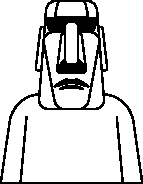
\includegraphics[height=\measurepage/2]{frontispice-moai.pdf}
% \end{center}



  %\null\vfill

  %\newpage
  \null\cleardoublepage
  \thispagestyle{empty}
  \pdfbookmark[0]{Post-scirptum}{Post-scriptum}
  \null\vfill           % Pression du haut pour condenser les informations de crédit en bas de la page.
  \addcredit{GFDL | \ccbysa}{Jeff Dahl}{https://commons.wikimedia.org/wiki/File:Blue\_crown.svg}
  \begin{flushright}
    \begin{minipage}[t]{0.6\textwidth}%
      \lettrine[lines=3]{V\llap{\raisebox{1.55ex}{
\includegraphics[height=0.92em]{khepresh_typographique.pdf}\hspace{-0.05em}}}}{oilà}
      %\lettrine[lines=3]{V\llap{\raisebox{0.68ex}{\includegraphics[height=1em]{Blue_crown.pdf}\hspace{-0.2em}}}}{\hspace{0.2em}oilà}
      désormais la pièce écrite, relue, et corrigée. Tandis que \texttt{ls -lt -{}-time=creation} me fait voir que les premiers jets de ce projets datent du 2023 avril 22, je me rend compte maintenant que nous sommes en septembre, soit près de sept mois \incise{gestation de guépards} après l’exhortation de mon ami. M’étant acquitté de la tache, j’espère Dereckson satisfait du résultat, car des rêves que je ferais, je ne lui en raconterais plus aucun !

      \vspace{0.5cm}

      \hfill 2023 septembre 3
    \end{minipage}%
  \end{flushright}

  \vfill\null                % Espace vértical.

  \backmatter
  \thispagestyle{empty}
  \null\cleardoublepage

  %\pdfbookmark[0]{Table des matières}{Table des matières}
  \fancyhead[LO]{Table des matières}
  \addcontentsline{toc}{chapter}{Table des matières}
  \tableofcontents

  \cleardoublepage
  \def\enotesize{\normalsize}
  \setenotez{list-name=Notes}
  \addcontentsline{toc}{chapter}{Notes}
  \printendnotes

  \null
  %\clearpage
  \null\vfill
  \thispagestyle{empty}
  \noindent{\Large Crédits}
  %\vspace{1em}

  \noindent\credittable{}

  \null
  \clearpage
  \null
  %\cleardoublepage
  \thispagestyle{empty}
  \pdfbookmark[0]{Quatrième de couverture}{quatrieme}
  \newgeometry{left=0cm,bottom=0cm,top=0cm,bottom=0cm,inner=0cm,outer=0cm}

  \null\vfill

    \noindent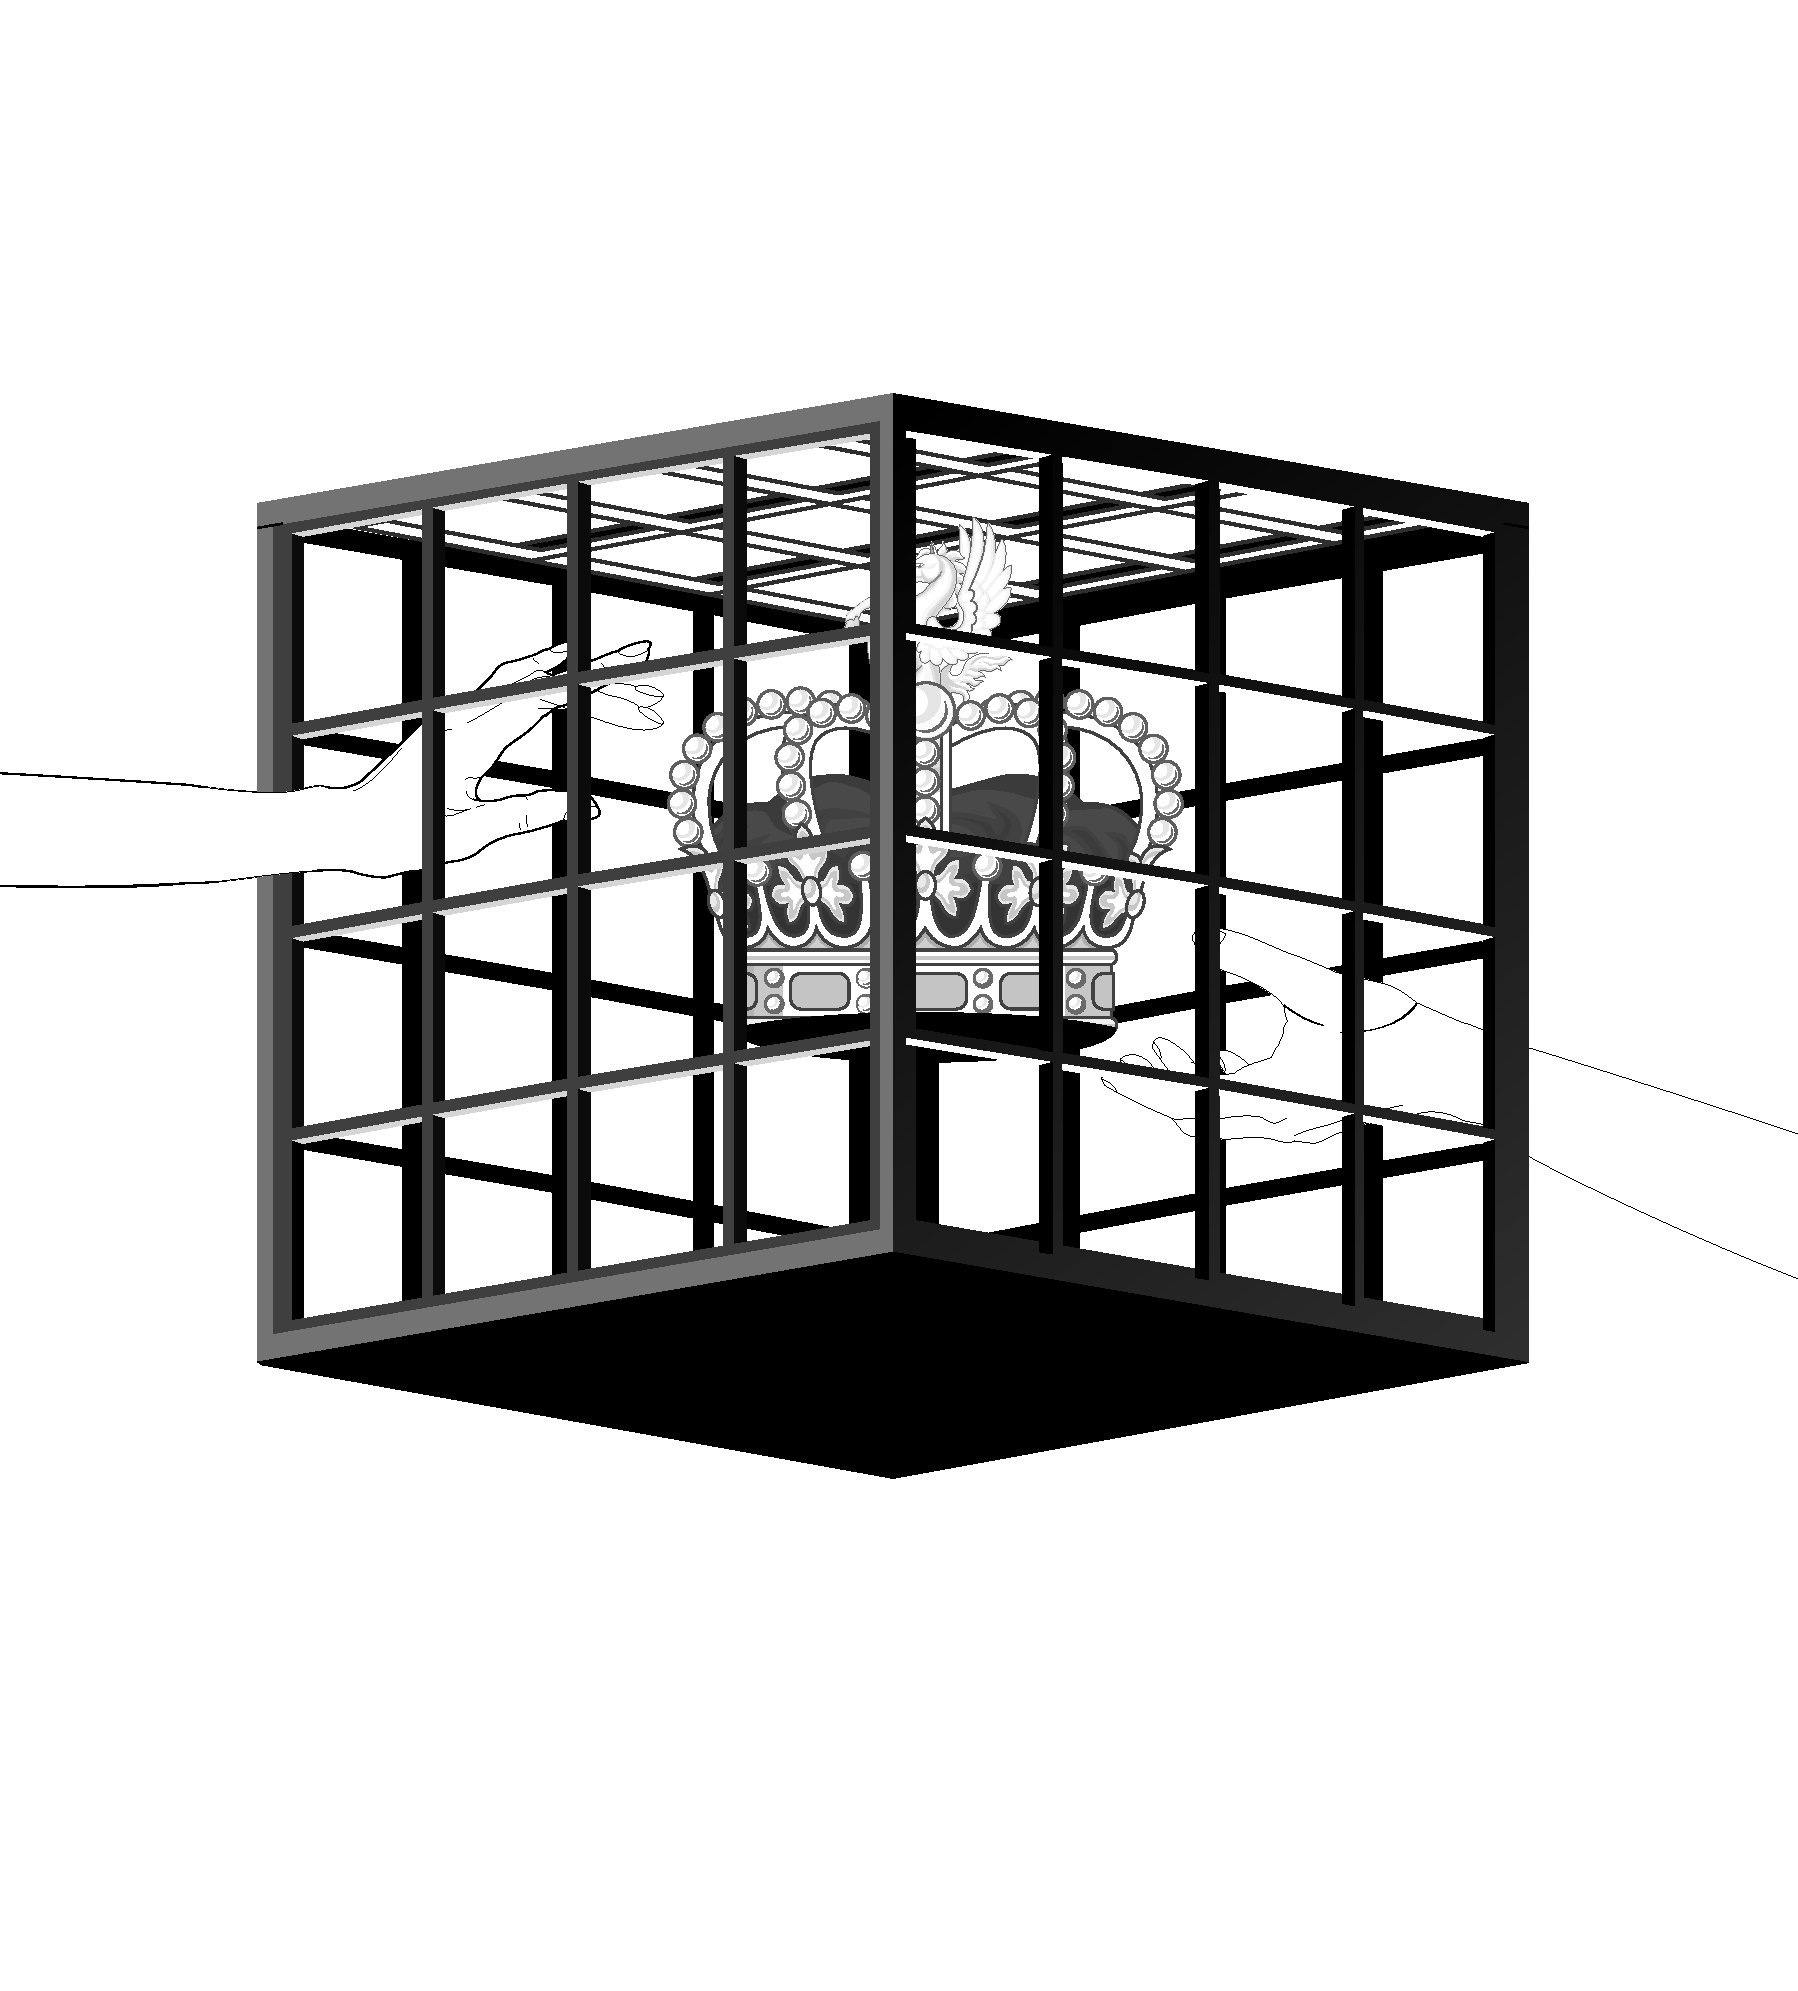
\includegraphics[width=\textwidth]{courrone-innacessible.pdf}

    

  \null\vfill


  %
  %
  %\printbibliography
  %
  %\glsaddall
  %\glossarystyle{tree}
  %\printglossary[title=Glossaire,toctitle=Glossaire]
  %
\end{document}
